\documentclass[11pt,a4paper]{report}

% ============================================================================
%  preambule.tex : paquets, mise en page, notations et environnements
%  (inclus dans main.tex par % ============================================================================
%  preambule.tex : paquets, mise en page, notations et environnements
%  (inclus dans main.tex par % ============================================================================
%  preambule.tex : paquets, mise en page, notations et environnements
%  (inclus dans main.tex par \input{preambule})
% ============================================================================

% ----------------------------------------------------------------------------
%  Polices et langue
% ----------------------------------------------------------------------------
\usepackage[T1]{fontenc}
\usepackage[utf8]{inputenc}     % à SUPPRIMER si lualatex/xelatex
\usepackage[french]{babel}
\usepackage{lmodern}
\usepackage{microtype}          % justification nettement meilleure

% ----------------------------------------------------------------------------
%  Géométrie
% ----------------------------------------------------------------------------
% 11 pt et 3 cm de marges latérales : environ 80 caractères par ligne,
% texte dense mais lisible.
\usepackage[a4paper,
            left=2.0cm, right=2.0cm, top=2.5cm, bottom=2.5cm,
            headheight=15pt]{geometry}

% ----------------------------------------------------------------------------
%  Mathématiques
% ----------------------------------------------------------------------------
\usepackage{amsmath, amssymb, amsthm, mathtools}
\usepackage{bm}
\usepackage{mathrsfs}

% ----------------------------------------------------------------------------
%  Flottants, tableaux, listes
% ----------------------------------------------------------------------------
\usepackage{graphicx}
\usepackage{float}
\usepackage{booktabs}
\usepackage{caption}
\usepackage{subcaption}         % APRÈS caption
\usepackage[inline]{enumitem}

% ----------------------------------------------------------------------------
%  Dessins
% ----------------------------------------------------------------------------
\usepackage{tikz}
\usetikzlibrary{arrows.meta, positioning, calc, angles, quotes,
    decorations.pathmorphing, patterns}

% ----------------------------------------------------------------------------
%  Couleurs, encadrés et liens
% ----------------------------------------------------------------------------
\usepackage{xcolor}
\definecolor{accent}{HTML}{1F3A5F}
\usepackage[most]{tcolorbox}

% Ligne « institution » de la page de titre.
\newcommand{\kicker}[1]{{\scshape\large\textcolor{accent}{#1}}}

\usepackage[colorlinks=true, linkcolor=accent, citecolor=accent,
            urlcolor=accent]{hyperref}
\usepackage{cleveref}           % IMPÉRATIVEMENT après hyperref

% ============================================================================
%  MISE EN PAGE
% ============================================================================

% --- 1. Titres ---------------------------------------------------------------
\usepackage{titlesec}

% Chapitre : « Chapitre » en petites capitales, gros numéro, titre
% en dessous, filet pour fermer.
\titleformat{\chapter}[display]
    {\normalfont}
    {%
        {\color{accent!55}\large\scshape\chaptertitlename}\;\;
        {\color{accent}\fontsize{52}{52}\selectfont\bfseries\thechapter}%
    }
    {10pt}
    {\color{accent}\Huge\bfseries}
    [\vspace{4mm}{\color{accent!40}\titlerule[1.4pt]}]
\titlespacing*{\chapter}{0pt}{20pt}{34pt}

% Structure : Chapitre -> I. -> 1. -> 1.1 -> a)
\setcounter{secnumdepth}{4}
\setcounter{tocdepth}{3}
\renewcommand{\thesection}{\Roman{section}.}
\renewcommand{\thesubsection}{\arabic{subsection}.}
\renewcommand{\thesubsubsection}{%
    \arabic{subsection}.\arabic{subsubsection}}
\renewcommand{\theparagraph}{\alph{paragraph})}

\titlespacing*{\section}{0pt}{2.2ex plus 1ex minus .2ex}{1.4ex plus .2ex}
\titlespacing*{\subsection}{0pt}{1.8ex plus 1ex minus .2ex}{1.0ex plus .2ex}
% a) : titre sur sa propre ligne
\titleformat{\paragraph}
    {\normalfont\normalsize\bfseries}{\theparagraph}{0.5em}{}
\titlespacing*{\paragraph}{0pt}{1.4ex plus .5ex minus .2ex}{0.6ex}

% --- 2. Flottants ------------------------------------------------------------
\renewcommand{\topfraction}{0.90}
\renewcommand{\bottomfraction}{0.75}
\renewcommand{\textfraction}{0.10}
\renewcommand{\floatpagefraction}{0.75}
\setcounter{topnumber}{3}
\setcounter{bottomnumber}{2}
\setcounter{totalnumber}{5}

% --- 3. Coupures de page -----------------------------------------------------
\widowpenalty=10000
\clubpenalty=10000
\raggedbottom

% --- 4. Listes et légendes ---------------------------------------------------
\setlist{itemsep=2pt, parsep=0pt, topsep=4pt}
\captionsetup{font=small, labelfont={bf,color=accent}, skip=6pt}

% --- 5. Accroche : phrase clé mise en exergue --------------------------------
% Usage : \begin{accroche} ... \end{accroche}
\newenvironment{accroche}[1][accent]{%
    \par\medskip\noindent
    \begingroup
    \color{#1}\itshape\large
    \rightskip=1.5em \leftskip=1.5em
    \parindent=0pt
    \hrule height 0.9pt\vspace{7pt}%
}{%
    \par\vspace{7pt}\hrule height 0.9pt
    \endgroup
    \par\medskip
}

% ============================================================================
%  NOTATIONS
% ============================================================================
% Vecteur : minuscule ou grecque, en gras italique
% (ex. \vect{u}, \vect{\omega}).
\newcommand{\vect}[1]{\bm{#1}}
% Matrice / tenseur : majuscule en gras droit (ex. \mat{R}, \mat{I}).
\newcommand{\mat}[1]{\mathbf{#1}}
% Quaternion : gras, souligné (ex. \quat{q} = (q_0, \vect{q})).
\newcommand{\quat}[1]{\underline{\bm{#1}}}
% Produit quaternionique : étoile centrée (\otimes est réservé au
% produit tensoriel).
\newcommand{\quatmul}{\ast}
% Repères : \rep{s} (sol), \rep{b} (solide).
\newcommand{\rep}[1]{\mathcal{R}_{#1}}
% Matrice antisymétrique associée à u : [u]_x v = u \wedge v
\newcommand{\hatx}[1]{[#1]_{\times}}
% Ensembles et opérateurs
\newcommand{\R}{\mathbb{R}}
\newcommand{\SO}{\mathrm{SO}(3)}
\newcommand{\Id}{\mat{I}}
\newcommand{\dd}{\mathrm{d}}
\newcommand{\ddt}{\frac{\dd}{\dd t}}
\newcommand{\pd}[2]{\frac{\partial #1}{\partial #2}}
\DeclareMathOperator{\rang}{rang}
\DeclareMathOperator{\Ker}{Ker}
\DeclareMathOperator{\Ima}{Im}

% ============================================================================
%  ENVIRONNEMENTS (numérotés par chapitre)
% ============================================================================
\theoremstyle{plain}
\newtheorem{theoreme}{Théorème}[chapter]
\newtheorem{corollaire}[theoreme]{Corollaire}
\newtheorem{proposition}[theoreme]{Proposition}
\newtheorem{lemme}[theoreme]{Lemme}
\theoremstyle{definition}
\newtheorem{definition}[theoreme]{Définition}
\newtheorem{hypotheses}[theoreme]{Hypothèses}
\newtheorem{exemple}[theoreme]{Exemple}
\theoremstyle{remark}
\newtheorem{remarque}[theoreme]{Remarque}
\newtheorem{note}[theoreme]{Note}
\renewcommand{\proofname}{Démonstration}
% Démonstration détaillée et preuve courte : même mise en forme
% (titre en italique, carré en fin).
\newenvironment{demonstration}[1][Démonstration]
    {\begin{proof}[#1]}{\end{proof}}
\newenvironment{preuve}[1][Preuve]
    {\begin{proof}[#1]}{\end{proof}}

% Couleurs des cadres : théorème en rouge, définition et hypothèses
% en vert, proposition, corollaire et lemme en bleu.
\definecolor{coulthm}{HTML}{A8322D}
\definecolor{couldef}{HTML}{2E7D32}
\definecolor{coulprop}{HTML}{1F5A9E}
\tcbset{
    cadre/.style={enhanced,colback=#1!7,colframe=#1!80,
        boxrule=0.6pt,leftrule=3pt,arc=1pt,left=6pt,right=6pt,
        before skip=6pt,after skip=6pt}}
\tcolorboxenvironment{theoreme}{cadre=coulthm}
\tcolorboxenvironment{definition}{cadre=couldef}
\tcolorboxenvironment{hypotheses}{cadre=couldef}
\tcolorboxenvironment{proposition}{cadre=coulprop}
\tcolorboxenvironment{corollaire}{cadre=coulprop}
\tcolorboxenvironment{lemme}{cadre=coulprop}
% Note : notation ou commentaire personnel, cadre gris.
\tcolorboxenvironment{note}{cadre=gray}

% Renvois \cref en français
\crefname{theoreme}{théorème}{théorèmes}
\Crefname{theoreme}{Théorème}{Théorèmes}
\crefname{corollaire}{corollaire}{corollaires}
\Crefname{corollaire}{Corollaire}{Corollaires}
\crefname{proposition}{proposition}{propositions}
\Crefname{proposition}{Proposition}{Propositions}
\crefname{lemme}{lemme}{lemmes}
\Crefname{lemme}{Lemme}{Lemmes}
\crefname{definition}{définition}{définitions}
\Crefname{definition}{Définition}{Définitions}
\crefname{hypotheses}{hypothèses}{hypothèses}
\Crefname{hypotheses}{Hypothèses}{Hypothèses}
\crefname{exemple}{exemple}{exemples}
\Crefname{exemple}{Exemple}{Exemples}
\crefname{remarque}{remarque}{remarques}
\Crefname{remarque}{Remarque}{Remarques}
\crefname{note}{note}{notes}
\Crefname{note}{Note}{Notes}
\newcommand{\creflastconjunction}{ et~}
)
% ============================================================================

% ----------------------------------------------------------------------------
%  Polices et langue
% ----------------------------------------------------------------------------
\usepackage[T1]{fontenc}
\usepackage[utf8]{inputenc}     % à SUPPRIMER si lualatex/xelatex
\usepackage[french]{babel}
\usepackage{lmodern}
\usepackage{microtype}          % justification nettement meilleure

% ----------------------------------------------------------------------------
%  Géométrie
% ----------------------------------------------------------------------------
% 11 pt et 3 cm de marges latérales : environ 80 caractères par ligne,
% texte dense mais lisible.
\usepackage[a4paper,
            left=2.0cm, right=2.0cm, top=2.5cm, bottom=2.5cm,
            headheight=15pt]{geometry}

% ----------------------------------------------------------------------------
%  Mathématiques
% ----------------------------------------------------------------------------
\usepackage{amsmath, amssymb, amsthm, mathtools}
\usepackage{bm}
\usepackage{mathrsfs}

% ----------------------------------------------------------------------------
%  Flottants, tableaux, listes
% ----------------------------------------------------------------------------
\usepackage{graphicx}
\usepackage{float}
\usepackage{booktabs}
\usepackage{caption}
\usepackage{subcaption}         % APRÈS caption
\usepackage[inline]{enumitem}

% ----------------------------------------------------------------------------
%  Dessins
% ----------------------------------------------------------------------------
\usepackage{tikz}
\usetikzlibrary{arrows.meta, positioning, calc, angles, quotes,
    decorations.pathmorphing, patterns}

% ----------------------------------------------------------------------------
%  Couleurs, encadrés et liens
% ----------------------------------------------------------------------------
\usepackage{xcolor}
\definecolor{accent}{HTML}{1F3A5F}
\usepackage[most]{tcolorbox}

% Ligne « institution » de la page de titre.
\newcommand{\kicker}[1]{{\scshape\large\textcolor{accent}{#1}}}

\usepackage[colorlinks=true, linkcolor=accent, citecolor=accent,
            urlcolor=accent]{hyperref}
\usepackage{cleveref}           % IMPÉRATIVEMENT après hyperref

% ============================================================================
%  MISE EN PAGE
% ============================================================================

% --- 1. Titres ---------------------------------------------------------------
\usepackage{titlesec}

% Chapitre : « Chapitre » en petites capitales, gros numéro, titre
% en dessous, filet pour fermer.
\titleformat{\chapter}[display]
    {\normalfont}
    {%
        {\color{accent!55}\large\scshape\chaptertitlename}\;\;
        {\color{accent}\fontsize{52}{52}\selectfont\bfseries\thechapter}%
    }
    {10pt}
    {\color{accent}\Huge\bfseries}
    [\vspace{4mm}{\color{accent!40}\titlerule[1.4pt]}]
\titlespacing*{\chapter}{0pt}{20pt}{34pt}

% Structure : Chapitre -> I. -> 1. -> 1.1 -> a)
\setcounter{secnumdepth}{4}
\setcounter{tocdepth}{3}
\renewcommand{\thesection}{\Roman{section}.}
\renewcommand{\thesubsection}{\arabic{subsection}.}
\renewcommand{\thesubsubsection}{%
    \arabic{subsection}.\arabic{subsubsection}}
\renewcommand{\theparagraph}{\alph{paragraph})}

\titlespacing*{\section}{0pt}{2.2ex plus 1ex minus .2ex}{1.4ex plus .2ex}
\titlespacing*{\subsection}{0pt}{1.8ex plus 1ex minus .2ex}{1.0ex plus .2ex}
% a) : titre sur sa propre ligne
\titleformat{\paragraph}
    {\normalfont\normalsize\bfseries}{\theparagraph}{0.5em}{}
\titlespacing*{\paragraph}{0pt}{1.4ex plus .5ex minus .2ex}{0.6ex}

% --- 2. Flottants ------------------------------------------------------------
\renewcommand{\topfraction}{0.90}
\renewcommand{\bottomfraction}{0.75}
\renewcommand{\textfraction}{0.10}
\renewcommand{\floatpagefraction}{0.75}
\setcounter{topnumber}{3}
\setcounter{bottomnumber}{2}
\setcounter{totalnumber}{5}

% --- 3. Coupures de page -----------------------------------------------------
\widowpenalty=10000
\clubpenalty=10000
\raggedbottom

% --- 4. Listes et légendes ---------------------------------------------------
\setlist{itemsep=2pt, parsep=0pt, topsep=4pt}
\captionsetup{font=small, labelfont={bf,color=accent}, skip=6pt}

% --- 5. Accroche : phrase clé mise en exergue --------------------------------
% Usage : \begin{accroche} ... \end{accroche}
\newenvironment{accroche}[1][accent]{%
    \par\medskip\noindent
    \begingroup
    \color{#1}\itshape\large
    \rightskip=1.5em \leftskip=1.5em
    \parindent=0pt
    \hrule height 0.9pt\vspace{7pt}%
}{%
    \par\vspace{7pt}\hrule height 0.9pt
    \endgroup
    \par\medskip
}

% ============================================================================
%  NOTATIONS
% ============================================================================
% Vecteur : minuscule ou grecque, en gras italique
% (ex. \vect{u}, \vect{\omega}).
\newcommand{\vect}[1]{\bm{#1}}
% Matrice / tenseur : majuscule en gras droit (ex. \mat{R}, \mat{I}).
\newcommand{\mat}[1]{\mathbf{#1}}
% Quaternion : gras, souligné (ex. \quat{q} = (q_0, \vect{q})).
\newcommand{\quat}[1]{\underline{\bm{#1}}}
% Produit quaternionique : étoile centrée (\otimes est réservé au
% produit tensoriel).
\newcommand{\quatmul}{\ast}
% Repères : \rep{s} (sol), \rep{b} (solide).
\newcommand{\rep}[1]{\mathcal{R}_{#1}}
% Matrice antisymétrique associée à u : [u]_x v = u \wedge v
\newcommand{\hatx}[1]{[#1]_{\times}}
% Ensembles et opérateurs
\newcommand{\R}{\mathbb{R}}
\newcommand{\SO}{\mathrm{SO}(3)}
\newcommand{\Id}{\mat{I}}
\newcommand{\dd}{\mathrm{d}}
\newcommand{\ddt}{\frac{\dd}{\dd t}}
\newcommand{\pd}[2]{\frac{\partial #1}{\partial #2}}
\DeclareMathOperator{\rang}{rang}
\DeclareMathOperator{\Ker}{Ker}
\DeclareMathOperator{\Ima}{Im}

% ============================================================================
%  ENVIRONNEMENTS (numérotés par chapitre)
% ============================================================================
\theoremstyle{plain}
\newtheorem{theoreme}{Théorème}[chapter]
\newtheorem{corollaire}[theoreme]{Corollaire}
\newtheorem{proposition}[theoreme]{Proposition}
\newtheorem{lemme}[theoreme]{Lemme}
\theoremstyle{definition}
\newtheorem{definition}[theoreme]{Définition}
\newtheorem{hypotheses}[theoreme]{Hypothèses}
\newtheorem{exemple}[theoreme]{Exemple}
\theoremstyle{remark}
\newtheorem{remarque}[theoreme]{Remarque}
\newtheorem{note}[theoreme]{Note}
\renewcommand{\proofname}{Démonstration}
% Démonstration détaillée et preuve courte : même mise en forme
% (titre en italique, carré en fin).
\newenvironment{demonstration}[1][Démonstration]
    {\begin{proof}[#1]}{\end{proof}}
\newenvironment{preuve}[1][Preuve]
    {\begin{proof}[#1]}{\end{proof}}

% Couleurs des cadres : théorème en rouge, définition et hypothèses
% en vert, proposition, corollaire et lemme en bleu.
\definecolor{coulthm}{HTML}{A8322D}
\definecolor{couldef}{HTML}{2E7D32}
\definecolor{coulprop}{HTML}{1F5A9E}
\tcbset{
    cadre/.style={enhanced,colback=#1!7,colframe=#1!80,
        boxrule=0.6pt,leftrule=3pt,arc=1pt,left=6pt,right=6pt,
        before skip=6pt,after skip=6pt}}
\tcolorboxenvironment{theoreme}{cadre=coulthm}
\tcolorboxenvironment{definition}{cadre=couldef}
\tcolorboxenvironment{hypotheses}{cadre=couldef}
\tcolorboxenvironment{proposition}{cadre=coulprop}
\tcolorboxenvironment{corollaire}{cadre=coulprop}
\tcolorboxenvironment{lemme}{cadre=coulprop}
% Note : notation ou commentaire personnel, cadre gris.
\tcolorboxenvironment{note}{cadre=gray}

% Renvois \cref en français
\crefname{theoreme}{théorème}{théorèmes}
\Crefname{theoreme}{Théorème}{Théorèmes}
\crefname{corollaire}{corollaire}{corollaires}
\Crefname{corollaire}{Corollaire}{Corollaires}
\crefname{proposition}{proposition}{propositions}
\Crefname{proposition}{Proposition}{Propositions}
\crefname{lemme}{lemme}{lemmes}
\Crefname{lemme}{Lemme}{Lemmes}
\crefname{definition}{définition}{définitions}
\Crefname{definition}{Définition}{Définitions}
\crefname{hypotheses}{hypothèses}{hypothèses}
\Crefname{hypotheses}{Hypothèses}{Hypothèses}
\crefname{exemple}{exemple}{exemples}
\Crefname{exemple}{Exemple}{Exemples}
\crefname{remarque}{remarque}{remarques}
\Crefname{remarque}{Remarque}{Remarques}
\crefname{note}{note}{notes}
\Crefname{note}{Note}{Notes}
\newcommand{\creflastconjunction}{ et~}
)
% ============================================================================

% ----------------------------------------------------------------------------
%  Polices et langue
% ----------------------------------------------------------------------------
\usepackage[T1]{fontenc}
\usepackage[utf8]{inputenc}     % à SUPPRIMER si lualatex/xelatex
\usepackage[french]{babel}
\usepackage{lmodern}
\usepackage{microtype}          % justification nettement meilleure

% ----------------------------------------------------------------------------
%  Géométrie
% ----------------------------------------------------------------------------
% 11 pt et 3 cm de marges latérales : environ 80 caractères par ligne,
% texte dense mais lisible.
\usepackage[a4paper,
            left=2.0cm, right=2.0cm, top=2.5cm, bottom=2.5cm,
            headheight=15pt]{geometry}

% ----------------------------------------------------------------------------
%  Mathématiques
% ----------------------------------------------------------------------------
\usepackage{amsmath, amssymb, amsthm, mathtools}
\usepackage{bm}
\usepackage{mathrsfs}

% ----------------------------------------------------------------------------
%  Flottants, tableaux, listes
% ----------------------------------------------------------------------------
\usepackage{graphicx}
\usepackage{float}
\usepackage{booktabs}
\usepackage{caption}
\usepackage{subcaption}         % APRÈS caption
\usepackage[inline]{enumitem}

% ----------------------------------------------------------------------------
%  Dessins
% ----------------------------------------------------------------------------
\usepackage{tikz}
\usetikzlibrary{arrows.meta, positioning, calc, angles, quotes,
    decorations.pathmorphing, patterns}

% ----------------------------------------------------------------------------
%  Couleurs, encadrés et liens
% ----------------------------------------------------------------------------
\usepackage{xcolor}
\definecolor{accent}{HTML}{1F3A5F}
\usepackage[most]{tcolorbox}

% Ligne « institution » de la page de titre.
\newcommand{\kicker}[1]{{\scshape\large\textcolor{accent}{#1}}}

\usepackage[colorlinks=true, linkcolor=accent, citecolor=accent,
            urlcolor=accent]{hyperref}
\usepackage{cleveref}           % IMPÉRATIVEMENT après hyperref

% ============================================================================
%  MISE EN PAGE
% ============================================================================

% --- 1. Titres ---------------------------------------------------------------
\usepackage{titlesec}

% Chapitre : « Chapitre » en petites capitales, gros numéro, titre
% en dessous, filet pour fermer.
\titleformat{\chapter}[display]
    {\normalfont}
    {%
        {\color{accent!55}\large\scshape\chaptertitlename}\;\;
        {\color{accent}\fontsize{52}{52}\selectfont\bfseries\thechapter}%
    }
    {10pt}
    {\color{accent}\Huge\bfseries}
    [\vspace{4mm}{\color{accent!40}\titlerule[1.4pt]}]
\titlespacing*{\chapter}{0pt}{20pt}{34pt}

% Structure : Chapitre -> I. -> 1. -> 1.1 -> a)
\setcounter{secnumdepth}{4}
\setcounter{tocdepth}{3}
\renewcommand{\thesection}{\Roman{section}.}
\renewcommand{\thesubsection}{\arabic{subsection}.}
\renewcommand{\thesubsubsection}{%
    \arabic{subsection}.\arabic{subsubsection}}
\renewcommand{\theparagraph}{\alph{paragraph})}

\titlespacing*{\section}{0pt}{2.2ex plus 1ex minus .2ex}{1.4ex plus .2ex}
\titlespacing*{\subsection}{0pt}{1.8ex plus 1ex minus .2ex}{1.0ex plus .2ex}
% a) : titre sur sa propre ligne
\titleformat{\paragraph}
    {\normalfont\normalsize\bfseries}{\theparagraph}{0.5em}{}
\titlespacing*{\paragraph}{0pt}{1.4ex plus .5ex minus .2ex}{0.6ex}

% --- 2. Flottants ------------------------------------------------------------
\renewcommand{\topfraction}{0.90}
\renewcommand{\bottomfraction}{0.75}
\renewcommand{\textfraction}{0.10}
\renewcommand{\floatpagefraction}{0.75}
\setcounter{topnumber}{3}
\setcounter{bottomnumber}{2}
\setcounter{totalnumber}{5}

% --- 3. Coupures de page -----------------------------------------------------
\widowpenalty=10000
\clubpenalty=10000
\raggedbottom

% --- 4. Listes et légendes ---------------------------------------------------
\setlist{itemsep=2pt, parsep=0pt, topsep=4pt}
\captionsetup{font=small, labelfont={bf,color=accent}, skip=6pt}

% --- 5. Accroche : phrase clé mise en exergue --------------------------------
% Usage : \begin{accroche} ... \end{accroche}
\newenvironment{accroche}[1][accent]{%
    \par\medskip\noindent
    \begingroup
    \color{#1}\itshape\large
    \rightskip=1.5em \leftskip=1.5em
    \parindent=0pt
    \hrule height 0.9pt\vspace{7pt}%
}{%
    \par\vspace{7pt}\hrule height 0.9pt
    \endgroup
    \par\medskip
}

% ============================================================================
%  NOTATIONS
% ============================================================================
% Vecteur : minuscule ou grecque, en gras italique
% (ex. \vect{u}, \vect{\omega}).
\newcommand{\vect}[1]{\bm{#1}}
% Matrice / tenseur : majuscule en gras droit (ex. \mat{R}, \mat{I}).
\newcommand{\mat}[1]{\mathbf{#1}}
% Quaternion : gras, souligné (ex. \quat{q} = (q_0, \vect{q})).
\newcommand{\quat}[1]{\underline{\bm{#1}}}
% Produit quaternionique : étoile centrée (\otimes est réservé au
% produit tensoriel).
\newcommand{\quatmul}{\ast}
% Repères : \rep{s} (sol), \rep{b} (solide).
\newcommand{\rep}[1]{\mathcal{R}_{#1}}
% Matrice antisymétrique associée à u : [u]_x v = u \wedge v
\newcommand{\hatx}[1]{[#1]_{\times}}
% Ensembles et opérateurs
\newcommand{\R}{\mathbb{R}}
\newcommand{\SO}{\mathrm{SO}(3)}
\newcommand{\Id}{\mat{I}}
\newcommand{\dd}{\mathrm{d}}
\newcommand{\ddt}{\frac{\dd}{\dd t}}
\newcommand{\pd}[2]{\frac{\partial #1}{\partial #2}}
\DeclareMathOperator{\rang}{rang}
\DeclareMathOperator{\Ker}{Ker}
\DeclareMathOperator{\Ima}{Im}

% ============================================================================
%  ENVIRONNEMENTS (numérotés par chapitre)
% ============================================================================
\theoremstyle{plain}
\newtheorem{theoreme}{Théorème}[chapter]
\newtheorem{corollaire}[theoreme]{Corollaire}
\newtheorem{proposition}[theoreme]{Proposition}
\newtheorem{lemme}[theoreme]{Lemme}
\theoremstyle{definition}
\newtheorem{definition}[theoreme]{Définition}
\newtheorem{hypotheses}[theoreme]{Hypothèses}
\newtheorem{exemple}[theoreme]{Exemple}
\theoremstyle{remark}
\newtheorem{remarque}[theoreme]{Remarque}
\newtheorem{note}[theoreme]{Note}
\renewcommand{\proofname}{Démonstration}
% Démonstration détaillée et preuve courte : même mise en forme
% (titre en italique, carré en fin).
\newenvironment{demonstration}[1][Démonstration]
    {\begin{proof}[#1]}{\end{proof}}
\newenvironment{preuve}[1][Preuve]
    {\begin{proof}[#1]}{\end{proof}}

% Couleurs des cadres : théorème en rouge, définition et hypothèses
% en vert, proposition, corollaire et lemme en bleu.
\definecolor{coulthm}{HTML}{A8322D}
\definecolor{couldef}{HTML}{2E7D32}
\definecolor{coulprop}{HTML}{1F5A9E}
\tcbset{
    cadre/.style={enhanced,colback=#1!7,colframe=#1!80,
        boxrule=0.6pt,leftrule=3pt,arc=1pt,left=6pt,right=6pt,
        before skip=6pt,after skip=6pt}}
\tcolorboxenvironment{theoreme}{cadre=coulthm}
\tcolorboxenvironment{definition}{cadre=couldef}
\tcolorboxenvironment{hypotheses}{cadre=couldef}
\tcolorboxenvironment{proposition}{cadre=coulprop}
\tcolorboxenvironment{corollaire}{cadre=coulprop}
\tcolorboxenvironment{lemme}{cadre=coulprop}
% Note : notation ou commentaire personnel, cadre gris.
\tcolorboxenvironment{note}{cadre=gray}

% Renvois \cref en français
\crefname{theoreme}{théorème}{théorèmes}
\Crefname{theoreme}{Théorème}{Théorèmes}
\crefname{corollaire}{corollaire}{corollaires}
\Crefname{corollaire}{Corollaire}{Corollaires}
\crefname{proposition}{proposition}{propositions}
\Crefname{proposition}{Proposition}{Propositions}
\crefname{lemme}{lemme}{lemmes}
\Crefname{lemme}{Lemme}{Lemmes}
\crefname{definition}{définition}{définitions}
\Crefname{definition}{Définition}{Définitions}
\crefname{hypotheses}{hypothèses}{hypothèses}
\Crefname{hypotheses}{Hypothèses}{Hypothèses}
\crefname{exemple}{exemple}{exemples}
\Crefname{exemple}{Exemple}{Exemples}
\crefname{remarque}{remarque}{remarques}
\Crefname{remarque}{Remarque}{Remarques}
\crefname{note}{note}{notes}
\Crefname{note}{Note}{Notes}
\newcommand{\creflastconjunction}{ et~}


% ============================================================================
\begin{document}
% ============================================================================

\begin{titlepage}
    \centering

    \vspace*{\stretch{1}}

    \kicker{École Polytechnique}\par
    \vspace{0.35cm}
    {\color{accent}\rule{0.35\textwidth}{0.6pt}}\par

    \vspace{1.6cm}
    % Logos : placer les fichiers dans le dossier puis décommenter.
    % \includegraphics[height=3cm]{Pantone.png}\par
    \vspace{3cm}

    \vspace{\stretch{1.4}}

    % --- titre ---------------------------------------------------------------
    {\color{accent}\rule{\textwidth}{1.1pt}}\par
    \vspace{0.85cm}

    {\Huge\bfseries
        La sphère de Chaplygin\par}

    \vspace{0.85cm}
    {\color{accent}\rule{\textwidth}{1.1pt}}\par

    \vspace{1.1cm}
    {\Large\itshape Modélisation, Simulation, Analyse de stabilité
    \par}
    \vspace{0.3cm}
    {\Large\itshape et Estimations des paramètres\par}
    \vspace{0.3cm}

    \vspace{\stretch{2}}

    % --- auteur ----------------------------------------------------------------
    {\large\scshape Duc Bui\par}
    \vspace{0.25cm}
    {\small\color{black!60} duc.bui@polytechnique.edu - duc.bui.2024@polytechnique.org\par}

    \vspace{0.9cm}
    % --- tuteur ----------------------------------------------------------------
    {\normalsize Tuteur : \textsc{Nicolas Petit}\par}
    \vspace{0.15cm}
    {\small Centre Automatique et Systèmes, École des Mines de Paris -
    PSL\par}

    \vspace{\stretch{1}}
    {\large Octobre 2026\par}

\end{titlepage}

\tableofcontents

% ============================================================================
\chapter*{Notations et Conventions}
\addcontentsline{toc}{chapter}{Notations et Conventions}
% ============================================================================

\section*{Notations}

\begin{itemize}
    \item \textbf{Vecteurs} : en gras, minuscules ou lettres grecques,
        par exemple $\vect{u}$, $\vect{v}$, $\vect{\omega}$.
    \item \textbf{Matrices et tenseurs} : majuscules en gras, par
        exemple $\mat{R}$, $\mat{A}$, le tenseur d'inertie $\mat{I}_C$,        $\Id$ désigne l'identité.
    \item \textbf{Quaternions} : en gras et soulignés, $\quat{q} =
        (q_0,\vect{q})$, de partie scalaire $q_0$ et de partie vectorielle
        $\vect{q}$, \\
        $\quatmul$ désigne le produit quaternionique.
    \item \textbf{Ensembles et groupes} :
    \begin{itemize}
        \item $\R^n$ : vecteurs colonnes à $n$ composantes ;
        \item $\mathcal{M}_{m,n}(\R)$ : matrices réelles $m\times n$,
            et $\mathcal{M}_n(\R) := \mathcal{M}_{n,n}(\R)$.
        \item $\mathcal{A}_n(\R) = \{\mat{A}\in\mathcal{M}_n(\R) :
            \mat{A}^T = -\mat{A}\}$ : matrices antisymétriques.
        \item $\mathrm{O}(n) = \{\mat{Q}\in\mathcal{M}_n(\R) :
            \mat{Q}^T\mat{Q} = \Id\}$ : groupe orthogonal.
        \item $\SO = \{\mat{R}\in\mathrm{O}(3) : \det\mat{R} = 1\}$ :
            groupe des rotations.
        \item $C^k$ : fonctions $k$ fois continûment différentiables.
    \end{itemize}
    \item \textbf{Opérateurs} : $\mat{A}^T$ est la transposée,
        $\Ker\mat{A}$, $\Ima\mat{A}$ et $\rang\mat{A}$ le noyau, l'image
        et le rang de $\mat{A}$.
    \item \textbf{Configuration} : $q$ désigne une configuration ou ses
        coordonnées généralisées. Ces colonnes de coordonnées, sans
        sens géométrique propre ($q$, $\dot q$, une perturbation
        $\eta$, un état $X$, un gradient $\nabla_q L$), restent en
        maigre, les matrices associées (jacobienne $\mat{J}_f$,
        hessienne $\mat{H}_f$) suivent la règle des matrices.
    \item \textbf{Produits} : $\langle\vect{u},\vect{v}\rangle =
        \vect{u}^T\vect{v}$ est le produit scalaire et
        $\vect{u}\wedge\vect{v}$ le produit vectoriel et
        $\vect{u}\otimes\vect{v} = \vect{u}\vect{v}^T$ le produit
        tensoriel. À $\vect{u}$ on
        associe la matrice antisymétrique $\hatx{\vect{u}}$ telle que
        $\hatx{\vect{u}}\vect{v} = \vect{u}\wedge\vect{v}$.
    \item \textbf{Dérivées} : $\dot{\vect{u}} = \ddt\vect{u}$,
        $\pd{L}{q}$ et $\nabla_q L$ désignent la dérivée partielle et le
        gradient par rapport à $q$.
\end{itemize}

\section*{Repères}

On considère deux repères orthonormés directs :
\begin{itemize}
    \item $\rep{s}$, lié au sol, supposé galiléen.
    \item $\rep{b}$, lié au solide.
\end{itemize}

Pour un vecteur $\vect{u}$, on note $\vect{u}_s$ et $\vect{u}_b$ ses
colonnes de composantes dans $\rep{s}$ et $\rep{b}$. Elles sont reliées
par
\[
    \vect{u}_s = \mat{R}\,\vect{u}_b,
    \qquad \mat{R} := \mat{R}_{b\to s}\in\SO,
\]
où les colonnes de $\mat{R}$ sont les axes du solide exprimés dans le
repère du sol.

La vitesse angulaire du solide par rapport au sol est notée
$\vect{\omega}$ lorsqu'elle est exprimée dans $\rep{b}$, et
$\vect{\Omega} = \mat{R}\,\vect{\omega}$ lorsqu'elle est exprimée dans
$\rep{s}$.

% ============================================================================
% ============================================================================
%  Chapitre 1 : Base théorique
%  Une partie par fichier, incluses dans l'ordre.
% ============================================================================
\chapter[Base théorique]{Bases mathématiques}

% ============================================================================
%  Chapitre 1, partie I : Vecteurs et matrices
% ============================================================================

% ----------------------------------------------------------------------------
\section{Vecteurs et matrices}
% ----------------------------------------------------------------------------

\subsection{Notations}

Le \emph{produit scalaire} de deux vecteurs s'écrit
\[
    \langle \vect{u},\vect{v}\rangle = \vect{u}^T\vect{v}
\]
Par exemple, la puissance d'une force $\vect{F}$ appliquée en un point
de vitesse $\vect{v}$ est
$\mathcal{P}_F = \langle\vect{F},\vect{v}\rangle = \vect{F}^T\vect{v}$

Le \emph{produit vectoriel} se calcule par un déterminant. Dans une base
orthonormée directe $\mathcal{B} = \{\vect{e}_1,\vect{e}_2,\vect{e}_3\}$,
avec $\vect{u} = (u_1,u_2,u_3)$ et $\vect{v} = (v_1,v_2,v_3)$ :
\[
    \vect{u}\wedge\vect{v}
    = \det\begin{pmatrix}
        \vect{e}_1 & \vect{e}_2 & \vect{e}_3\\
        u_1 & u_2 & u_3\\
        v_1 & v_2 & v_3
    \end{pmatrix}
    = \begin{pmatrix}
        u_2v_3 - u_3v_2\\
        u_3v_1 - u_1v_3\\
        u_1v_2 - u_2v_1
    \end{pmatrix}_{\mathcal{B}},
\]
le déterminant étant développé selon la première ligne. On en
déduit, pour tout $\vect{w}$, le produit mixte
\[
    (\vect{u}\wedge\vect{v})^T\vect{w}
    = \det(\vect{u},\vect{v},\vect{w})
\]

Une matrice de rotation $\mat{R}$ est orthogonale :
\[
    \mat{R}^T\mat{R} = \Id,
    \qquad
    \mat{R}^{-1} = \mat{R}^T,
\]
et conserve donc le produit scalaire. L'orientation d'un solide est
décrite par une matrice de
\[
    \SO = \left\{\mat{R}\in\mathcal{M}_3(\R) :
    \mat{R}^T\mat{R} = \Id,\ \det\mat{R} = 1\right\}
\]

\subsection{Les théorèmes importants}

\subsubsection{Théorème spectral}

\paragraph{Énoncé}

\begin{theoreme}[Théorème spectral]
    Si $\mat{S}$ est une matrice symétrique réelle, il existe une base
    orthonormée $(\vect{e}_i)$ telle que
    $\mat{S}\vect{e}_i = \lambda_i\vect{e}_i$. Autrement dit,
    \[
        \mat{S} = \mat{Q}\mat{D}\mat{Q}^T,
        \qquad \mat{Q}\in\mathrm{O}(n),
        \quad \text{avec} \quad \mat{D} \text{ diagonale}
    \]
\end{theoreme}

\paragraph{Exemple avec la matrice d'inertie}

La matrice d'inertie $\mat{J}$ est toujours symétrique par définition, elle se diagonalise donc
automatiquement sur ses axes propres.
Avec $\vect{L} = \mat{J}\vect{\omega}$, l'énergie cinétique de
rotation s'écrit
\[
    T_{\mathrm{rot}}
    = \tfrac12\langle\vect{\omega},\vect{L}\rangle
    = \tfrac12\,\vect{\omega}^T\mat{J}\vect{\omega}
\]
Dans la base propre $\mathcal{B}_J = \{\vect{e}_1,\vect{e}_2,\vect{e}_3\}$,
$\mat{J} = \mathrm{diag}(J_1,J_2,J_3)$ et, pour
$\vect{\omega} = \sum_i \omega_i\vect{e}_i$,
\[
    T_{\mathrm{rot}}
    = \tfrac12\left(J_1\omega_1^2 + J_2\omega_2^2 + J_3\omega_3^2\right)
\]

\subsubsection{Orthogonalité noyau-image}

\paragraph{Énoncé}

\begin{theoreme}[Orthogonalité noyau-image]
    Pour $\mat{A}\in\mathcal{M}_{m,n}(\R)$,
    $(\Ker\mat{A})^\perp = \Ima(\mat{A}^T)$. Autrement dit, pour $\vect{r} \in \R^n$
    \[
        \bigl(\forall\vect{v},\ \mat{A}\vect{v} = 0
        \Rightarrow \vect{r}^T\vect{v} = 0\bigr)
        \longleftrightarrow
        \exists\,\vect{\lambda}\in\R^m,\
        \vect{r} = \mat{A}^T\vect{\lambda}
    \]
\end{theoreme}

\paragraph{Intuition mécanique}

Par exemple, si les vitesses admissibles vérifient $\mat{A}\vect{v} = 0$, alors
$\Ker\mat{A}$ est l'ensemble des directions autorisées, et
$(\Ker\mat{A})^\perp$, qui rassemble tous les vecteurs orthogonaux 
à ces direction, est formé des combinaisons linéaires des colonnes
de $\mat{A}^T$. Une réaction qui ne travaille dans aucune direction
autorisée est donc de la forme $\mat{A}^T\vect{\lambda}$. Une interprétation plus proche 
de la mécanique classique sera donnée dans les parties suivantes.

\begin{exemple}[Point attaché au plan $z = 0$]
    La contrainte est $v_z = 0$, soit
    $\mat{A} = \begin{pmatrix} 0 & 0 & 1 \end{pmatrix}$ Alors
    \[
        \Ker\mat{A} = \{(v_x,v_y,0)\},
        \qquad
        \Ima\mat{A}^T = \{(0,0,\lambda)\}
    \]
    Une liaison idéale (sans frottement) ne fournit aucune puissance
    pour tout $\vect{v}\in\Ker\mat{A}$ : $\vect{R}^T\vect{v} = 0$,
    donc $\vect{R} = \mat{A}^T\lambda$ La réaction est normale au
    plan.
\end{exemple}
   % I.  Vecteurs et matrices
% ============================================================================
%  Chapitre 1, partie II : Analyse, variations et EDOs
% ============================================================================
\newpage
% ----------------------------------------------------------------------------
\section{Analyse, variations et EDOs}
% ----------------------------------------------------------------------------

L'objectif de cette partie est de comprendre
les bases mathématiques qui permettent de passer
d'un \emph{lagrangien} aux équations de mouvement.
On considère $q\in U\subset\R^n$ ouvert
et
\[
    L : U\times\R^n\times I\to\R,
    \qquad (q,v,t)\mapsto L(q,v,t)
\]

\subsection{Différentiabilité en dimension finie}

\begin{definition}[Différentiabilité]
    $f$ est \emph{différentiable} en $x$ s'il existe une application
    linéaire $Df(x)$ telle que
    \[
        f(x+h) = f(x) + Df(x)\,h + o(\|h\|)
    \]
    La matrice de $Df(x)$ est la \emph{jacobienne} $\mat{J}_f(x)$. Si
    $f$ est à valeurs scalaires, on note $\nabla f(x)$ son
    \emph{gradient}.
\end{definition}

\subsection{Règle de chaîne et dérivation le long d'une trajectoire}

\paragraph{Règle de chaîne}

\begin{theoreme}[Règle de chaîne]
    \[
        D(f\circ g)(x) = Df(g(x))\circ Dg(x),
        \qquad
        \mat{J}_{f\circ g}(x) = \mat{J}_f(g(x))\,\mat{J}_g(x),
    \]
    et pour $f$ scalaire,
    $\nabla(f\circ g)(x) = \mat{J}_g(x)^T\,\nabla f(g(x))$.
\end{theoreme}

\paragraph{Dérivée le long d'une trajectoire}

Le long d'une trajectoire $t\mapsto q(t)$,
\[
    \ddt F(q(t),t) = \partial_t F + \nabla_q F\cdot\dot q
\]
Pour $L$, on dérive d'abord en traitant $q$ et $v$ comme des
variables \emph{indépendantes}, puis on évalue en $v = \dot q$ :
\[
    \ddt L = \partial_t L + (\nabla_q L)^T\dot q
    + (\nabla_v L)^T\ddot q
\]

\begin{exemple}[$L = \tfrac12 M(q)v^2 - V(q)$]
    Ici $\partial_t L = 0$, et $v = \dot q$ est indépendant de $q$ :
    \[
        \pd{L}{v} = M(q)\,v,
        \qquad
        \pd{L}{q} = \tfrac12 M'(q)\,v^2 - V'(q),
        \qquad
        \ddt\pd{L}{\dot q} = M'(q)\,\dot q^2 + M(q)\,\ddot q
    \]
    L'équation d'Euler-Lagrange donne
    \[
        M(q)\,\ddot q + \tfrac12 M'(q)\,\dot q^2 + V'(q) = 0
    \]
\end{exemple}


\subsection{Dérivées secondes, Schwarz et Taylor}

\begin{theoreme}[Schwarz]
    Si $f$ est de classe $C^2$, alors
    $\dfrac{\partial^2 f}{\partial x_i\partial x_j}
    = \dfrac{\partial^2 f}{\partial x_j\partial x_i}$ :
    la \emph{hessienne} $\mat{H}_f := \nabla^2 f$ est donc symétrique.
\end{theoreme}

\begin{theoreme}[Taylor à l'ordre 2]
    \[
        f(x+h) = f(x) + \nabla f(x)^T h
        + \tfrac12\, h^T\mat{H}_f(x)\,h + o(\|h\|^2)
    \]
\end{theoreme}

\subsection{Fonctionnelles et première variation}

\begin{definition}[Fonctionnelle]
    Une fonction ordinaire associe une valeur à un point. 
    Une \emph{fonctionnelle} associe une valeur à une fonction
    entière, et on se restreint à : $S : \mathcal{F}\to\R$, où
    \[
        \mathcal{F} = \{q : [t_0,t_1]\to U
        \text{ de classe } C^2\}
    \]
    Les éléments de $\mathcal{F}$ sont appelés \emph{chemins} ou
    \emph{trajectoires admissibles}. On considère notamment la
    fonctionnelle
    \[
        S[q] = \int_{t_0}^{t_1} L(q,\dot q,t)\,\dd t
    \]
\end{definition}

\begin{definition}[Première variation]
    Pour une perturbation $\eta$ et $q_\varepsilon (t) = q(t) + \varepsilon\eta(t)$,
    \[
        \delta S[q;\eta]
        = \frac{\dd}{\dd\varepsilon}
        S[q(t) + \varepsilon\eta(t)]\Big|_{\varepsilon=0}
    \]
\end{definition}

On note $\delta q = \eta$, et $\delta\dot q = \dot\eta = \ddt\delta q$

\begin{proposition}[Calcul de la première variation]
    Si $L$ est de classe $C^2$, $q\in\mathcal{F}$ et $\eta$ de classe
    $C^1$, alors
    \begin{equation}\label{eq-premiere-variation}
        \delta S[q;\eta]
        = \int_{t_0}^{t_1}\sum_{i=1}^{n}
        \left(\pd{L}{q_i}\,\eta_i + \pd{L}{\dot q_i}\,\dot\eta_i\right)
        \dd t
        = \int_{t_0}^{t_1}
        \left(\nabla_q L^T\eta + \nabla_{\dot q} L^T\dot\eta\right)
        \dd t
    \end{equation}
\end{proposition}

\begin{demonstration}
    On a $q_\varepsilon(t) = q(t) + \varepsilon\eta(t)$, donc
    $\dot q_\varepsilon(t) = \dot q(t) + \varepsilon\dot\eta(t)$ La
    fonctionnelle associée à $q_\varepsilon$ est
    \[
        S[q_\varepsilon] = \int_{t_0}^{t_1}
        L(q+\varepsilon\eta,\dot q+\varepsilon\dot\eta,t)\,\dd t
    \]
    Comme $L$ est $C^2$ et l'intervalle est borné, on peut dériver
    sous l'intégrale :
    \[
        \delta S[q;\eta]
        = \frac{\dd}{\dd\varepsilon}\left(\int_{t_0}^{t_1}
        L(q+\varepsilon\eta,\dot q+\varepsilon\dot\eta,t)\,\dd t\right)
        \bigg|_{\varepsilon=0}
        = \int_{t_0}^{t_1}\frac{\dd}{\dd\varepsilon}
        L(q+\varepsilon\eta,\dot q+\varepsilon\dot\eta,t)
        \Big|_{\varepsilon=0}\dd t
    \]
    On considère l'intégrande. Par la règle de chaîne, en traitant $q$
    et $\dot q$ comme des \textbf{variables indépendantes},
    \[
        \frac{\dd}{\dd\varepsilon}L(q_\varepsilon,\dot q_\varepsilon,t)
        \Big|_{\varepsilon=0}
        = \left(\pd{L}{q}\,\pd{q_\varepsilon}{\varepsilon}
        + \pd{L}{\dot q}\,\pd{\dot q_\varepsilon}{\varepsilon}\right)
        \bigg|_{\varepsilon=0}
        = \pd{L}{q}\,\eta + \pd{L}{\dot q}\,\dot\eta,
    \]
    car $\partial_\varepsilon q_\varepsilon = \eta$ et
    $\partial_\varepsilon\dot q_\varepsilon = \dot\eta$ En écrivant
    les composantes et en intégrant, on obtient
    \eqref{eq-premiere-variation}.
\end{demonstration}

\subsection{Intégration par parties et lemme fondamental du calcul variationnel}

\paragraph{Intégration par parties}

\[
    \int_{t_0}^{t_1} p^T\dot\eta\,\dd t
    = \bigl[p^T\eta\bigr]_{t_0}^{t_1}
    - \int_{t_0}^{t_1} \dot p^T\eta\,\dd t
\]
Si les extrémités sont fixées, $\eta(t_0) = \eta(t_1) = 0$ et le
terme de bord disparaît.

\paragraph{Lemme fondamental du calcul variationnel}

\begin{definition}[Support]
    Le \emph{support} d'une fonction $\eta$ définie sur un ouvert
    $\Omega$ est l'adhérence de l'ensemble où elle ne s'annule pas :
    \[
        \operatorname{supp}\eta
        = \overline{\{t\in\Omega : \eta(t)\neq 0\}}
    \]
    $\eta$ est \emph{à support compact dans} $\Omega$ si
    $\operatorname{supp}\eta$ est un compact inclus dans $\Omega$,
    en particulier $\eta$ est nulle au voisinage du bord de $\Omega$.
\end{definition}

\begin{lemme}[Lemme de Du Bois-Reymond]
    Soit $f : [t_0,t_1]\to\R$ continue. Si
    \[
        \int_{t_0}^{t_1} f(t)\,\eta(t)\,\dd t = 0
        \qquad \forall\,\eta\in C_c^\infty(]t_0,t_1[,\R),
    \]
    c'est-à-dire pour toute fonction $\eta$ de classe $C^\infty$ 
    à support compact dans $]t_0,t_1[$, alors
    \[
        f = 0 \quad \text{sur } [t_0,t_1]
    \]
\end{lemme}
Ici, on fait une petite démonstration de ce résultat important.
\begin{demonstration}
    On note $\Omega = \,]t_0,t_1[$. Par l'absurde, supposons qu'il
    existe $t^*\in\Omega$ tel que $f(t^*)\neq 0$, et, sans perte de généralité
    , on suppose que $f(t^*) > 0$ (sinon on prend $-f$). Comme $f$ est continue, il existe un
    voisinage ouvert $\omega = \subset\Omega$ sur lequel
    $f > 0$.

    Soit $\eta\in C_c^\infty(\Omega)$ positive, non nulle, à support dans
    $\omega$. Comme $\eta$ est nulle en dehors de $\omega$,
    \[
        0 = \int_\Omega f\,\eta\,\dd t = \int_\omega f\,\eta\,\dd t
    \]
    Or sur $\omega$, $f > 0$ et $\eta\geq 0$ non nulle, donc
    $f\,\eta$ est continue, positive et non identiquement nulle, d'où
    $\int_\omega f\,\eta\,\dd t > 0$ :
    contradiction. Ainsi $f = 0$ sur $\Omega$, puis sur $[t_0,t_1]$ par
    continuité.
\end{demonstration}

En appliquant l'intégration par parties à
\eqref{eq-premiere-variation} avec $p = \nabla_{\dot q}L$ :
\[
    \delta S[q;\eta] = \int_{t_0}^{t_1}
    \left(\nabla_q L - \ddt\nabla_{\dot q} L\right)^T\eta\,\dd t
\]

\begin{corollaire}[Équations d'Euler-Lagrange]
    Si $\delta S[q;\eta] = 0$ pour tout $\eta$ nulle aux extrémités,
    \[
        \ddt\nabla_{\dot q} L - \nabla_q L = 0
    \]
\end{corollaire}

\subsection{Problème de Cauchy}

On considère le problème de Cauchy
\[
    \dot X = f(X,t),
    \qquad X(t_0) = X_0
\]

\begin{theoreme}[Cauchy-Lipschitz]
    Si $f$ est continue et localement lipschitzienne en $X$, il existe
    une unique solution maximale, définie sur un intervalle ouvert
    contenant $t_0$.
\end{theoreme}

\subsection{Linéarisation et intégrales premières}

\paragraph{Équation variationnelle}

Soit une famille de solutions $X_\varepsilon$ autour d'une solution
de référence $X_* = X_{\varepsilon=0}$ L'écart
$\xi = \partial_\varepsilon X_\varepsilon|_{\varepsilon=0}$ vérifie
l'\emph{équation variationnelle}
\[
    \dot\xi = \mat{A}(t)\,\xi,
    \qquad \mat{A}(t) := \mat{J}_f(X_*(t),t),
\]
où la jacobienne est prise par rapport à $X$.

\paragraph{Intégrale première}

\begin{definition}[Intégrale première]
    $E(X,t)$ est une \emph{intégrale première} si elle est constante
    le long des solutions :
    \[
        \ddt E = \partial_t E + (\nabla_X E)^T f = 0
    \]
\end{definition}
   % II. Analyse, variations et EDOs

% ============================================================================
%  Chapitre 2 : Base théorique de la mécanique analytique
%  Une partie par fichier, incluses dans l'ordre.
% ============================================================================
\chapter[Mécanique analytique]{Base théorique de la\\
mécanique analytique}

% ============================================================================
%  Chapitre 2, partie I : Mécanique du solide
%  (manuscrit P1, p. 13 à 19)
% ============================================================================

% ----------------------------------------------------------------------------
\section{Mécanique du solide}
% ----------------------------------------------------------------------------

On considère un solide $\mathcal{B}$ de masse $m$, de centre de masse
$C$, et un point courant $P\in\mathcal{B}$ de masse élémentaire
$\dd m$.

% ----------------------------------------------------------------------------
\subsection{Centre de masse et cinématique}

\subsubsection{Centre de masse}

\begin{definition}[Centre de masse]
    Le \emph{centre de masse} $C$ est défini par
    \[
        \overrightarrow{OC}
        = \frac{1}{m}\int_{\mathcal{B}} \overrightarrow{OP}\,\dd m,
        \qquad m = \int_{\mathcal{B}} \dd m
    \]
\end{definition}

En écrivant $\overrightarrow{OP} = \overrightarrow{OC}
+ \overrightarrow{CP}$,
\[
    \overrightarrow{OC}
    = \frac{1}{m}\int_{\mathcal{B}} \overrightarrow{OC}\,\dd m
    + \frac{1}{m}\int_{\mathcal{B}} \overrightarrow{CP}\,\dd m
    = \overrightarrow{OC}
    + \frac{1}{m}\int_{\mathcal{B}} \overrightarrow{CP}\,\dd m
    \longleftrightarrow
    \int_{\mathcal{B}} \overrightarrow{CP}\,\dd m = \vect{0}
\]

\subsubsection{Champ des vitesses d'un solide}

Soient deux points $A$ et $B$ fixes dans un repère $\rep{j}$ en
mouvement par rapport à un repère $\rep{i}$ d'origine $O_i$. La vitesse
de $B$ par rapport à $\rep{i}$ est par définition
\[
    \vect{v}_{B/i}
    = \left(\ddt\overrightarrow{O_iB}\right)_{\rep{i}}
    = \left(\ddt\overrightarrow{O_iA}\right)_{\rep{i}}
    + \left(\ddt\overrightarrow{AB}\right)_{\rep{i}}
    = \vect{v}_{A/i}
    + \left(\ddt\overrightarrow{AB}\right)_{\rep{i}}
\]

\begin{theoreme}[Dérivation en base mobile]
    Soient deux repères $\rep{i}$ et $\rep{j}$, $\rep{j}$ étant en
    mouvement par rapport à $\rep{i}$ avec la vitesse angulaire
    $\vect{\Omega}_{j/i}$. Pour deux points $A$ et $B$,
    \[
        \left(\ddt\overrightarrow{AB}\right)_{\rep{i}}
        = \left(\ddt\overrightarrow{AB}\right)_{\rep{j}}
        + \vect{\Omega}_{j/i}\wedge\overrightarrow{AB}
    \]
\end{theoreme}

Si $A$ et $B$ sont fixes dans $\rep{j}$, $\overrightarrow{AB}$ y est
constant et
\[
    \vect{v}_{B/i} = \vect{v}_{A/i}
    + \vect{\Omega}_{j/i}\wedge\overrightarrow{AB}
\]
Appliquée au solide, avec $\vect{\Omega}$ sa vitesse angulaire, cette
relation donne le \emph{champ des vitesses}
\[
    \vect{v}_P = \vect{v}_C + \vect{\Omega}\wedge\overrightarrow{CP}
\]

\subsubsection{Champ des accélérations}

En dérivant le champ des vitesses dans $\rep{i}$,
\[
    \vect{a}_P = \dot{\vect{v}}_P
    = \dot{\vect{v}}_C
    + \dot{\vect{\Omega}}\wedge\overrightarrow{CP}
    + \vect{\Omega}\wedge
    \left(\ddt\overrightarrow{CP}\right)_{\rep{i}}
\]
et, puisque $\bigl(\ddt\overrightarrow{CP}\bigr)_{\rep{i}}
= \vect{\Omega}\wedge\overrightarrow{CP}$,

\begin{proposition}[Champ des accélérations]
    \[
        \vect{a}_P = \vect{a}_C
        + \dot{\vect{\Omega}}\wedge\overrightarrow{CP}
        + \vect{\Omega}\wedge\bigl(\vect{\Omega}\wedge
        \overrightarrow{CP}\bigr)
    \]
\end{proposition}

% ----------------------------------------------------------------------------
\subsection{Quantité de mouvement et loi de Newton}

\begin{definition}[Quantité de mouvement du solide]
    \[
        \vect{P} = \int_{\mathcal{B}} \vect{v}_P\,\dd m
    \]
\end{definition}

Avec le champ des vitesses et $\int_{\mathcal{B}}\overrightarrow{CP}\,
\dd m = \vect{0}$, on obtient $\vect{P} = m\,\vect{v}_C$

\begin{theoreme}[Loi de Newton]
    Dans un repère galiléen, si $\vect{F}_{\mathrm{ext}}$ est la
    résultante des actions extérieures,
    \[
        \ddt\vect{P} = \vect{F}_{\mathrm{ext}},
        \qquad\text{donc}\qquad
        m\,\vect{a}_C = \vect{F}_{\mathrm{ext}}
    \]
\end{theoreme}

% ----------------------------------------------------------------------------
\subsection{Tenseur d'inertie et moment cinétique}

\begin{definition}[Moment cinétique]
    Le \emph{moment cinétique} au centre de masse est
    \[
        \vect{L}_C = \int_{\mathcal{B}}
        \overrightarrow{CP}\wedge\vect{v}_P\,\dd m
    \]
\end{definition}

En posant $\vect{r} = \overrightarrow{CP}$, le champ des vitesses donne
\[
    \vect{L}_C = \int_{\mathcal{B}}
    \vect{r}\wedge(\vect{\Omega}\wedge\vect{r})\,\dd m,
    \qquad\text{car}\qquad
    \int_{\mathcal{B}} \vect{r}\wedge\vect{v}_C\,\dd m
    = \left(\int_{\mathcal{B}}\vect{r}\,\dd m\right)\wedge\vect{v}_C
    = \vect{0}
\]

\begin{proposition}[Double produit vectoriel]
    \[
        \vect{r}\wedge(\vect{\Omega}\wedge\vect{r})
        = \|\vect{r}\|^2\vect{\Omega} - \vect{r}\,(\vect{r}^T\vect{\Omega})
        = \bigl(\|\vect{r}\|^2\Id - \vect{r}\vect{r}^T\bigr)\vect{\Omega}
    \]
\end{proposition}

On obtient alors
\[
    \vect{L}_C = \left(\int_{\mathcal{B}}
    \bigl(\|\vect{r}\|^2\Id - \vect{r}\vect{r}^T\bigr)\dd m\right)
    \vect{\Omega}
\]

\begin{definition}[Tenseur d'inertie autour de $C$]
    \[
        \mat{I}_C = \int_{\mathcal{B}}
        \bigl(\|\vect{r}\|^2\Id - \vect{r}\vect{r}^T\bigr)\dd m,
        \qquad
        \vect{L}_C = \mat{I}_C\,\vect{\Omega}
    \]
\end{definition}

\begin{theoreme}[Propriétés du tenseur d'inertie]
    \leavevmode
    \begin{itemize}
        \item $\mat{I}_C$ est symétrique : $\mat{I}_C^T = \mat{I}_C$ ;
        \item $\mat{I}_C$ est positive : pour tout $\vect{u}\in\R^3$,  c'est-à-dire
            \[
                \vect{u}^T\mat{I}_C\,\vect{u}
                = \int_{\mathcal{B}}\|\vect{r}\wedge\vect{u}\|^2\,\dd m
                \geq 0
            \]
    \end{itemize}
    Par le théorème spectral, $\mat{I}_C$ est donc diagonalisable en
    base orthonormée : dans la base des \emph{axes principaux
    d'inertie},
    \[
        \mat{I}_C = \mathrm{diag}(I_1,I_2,I_3),
        \qquad I_1, I_2, I_3 \geq 0
    \]
\end{theoreme}

% ----------------------------------------------------------------------------
\subsection{Théorème du moment cinétique}

On note $\vect{M}_C^{\mathrm{ext}}$ le moment résultant des actions
extérieures autour de $C$.

\begin{theoreme}[Théorème du moment cinétique]
    \[
        \left(\ddt\vect{L}_C\right)_{\text{galiléen}}
        = \vect{M}_C^{\mathrm{ext}}
    \]
\end{theoreme}

% ----------------------------------------------------------------------------
\subsection{Théorèmes de König}

\begin{theoreme}[Premier théorème de König]
    Pour tout point $A$,
    \[
        \vect{L}_A = \vect{L}_C
        + \overrightarrow{AC}\wedge m\,\vect{v}_C
    \]
\end{theoreme}

\begin{theoreme}[Deuxième théorème de König]
    L'énergie cinétique d'un corps rigide est
    \[
        T = E_K + E_K^*,
        \qquad
        E_K = \tfrac12\,m\,\|\vect{v}_C\|^2,
        \qquad
        E_K^* = \tfrac12\,\vect{\Omega}^T\mat{I}_C\,\vect{\Omega}
    \]
\end{theoreme}

\begin{preuve}
    Avec $\vect{v}_P = \vect{v}_C + \vect{\Omega}\wedge\vect{r}$,
    \begin{align*}
        T &= \frac12\int_{\mathcal{B}}\|\vect{v}_P\|^2\,\dd m
        = \frac12\int_{\mathcal{B}}
        \langle\vect{v}_C + \vect{\Omega}\wedge\vect{r},
        \vect{v}_C + \vect{\Omega}\wedge\vect{r}\rangle\,\dd m\\
        &= \frac12\,m\,\|\vect{v}_C\|^2
        + \frac12\int_{\mathcal{B}}\|\vect{\Omega}\wedge\vect{r}\|^2
        \,\dd m
        + \Bigl\langle\vect{v}_C,\ \vect{\Omega}\wedge
        \underbrace{\int_{\mathcal{B}}\vect{r}\,\dd m}_{=\,\vect{0}}
        \Bigr\rangle
    \end{align*}
    Enfin, d'après les propriétés du tenseur d'inertie,
    \[
        \frac12\int_{\mathcal{B}}\|\vect{\Omega}\wedge\vect{r}\|^2\,\dd m
        = \frac12\int_{\mathcal{B}}\|\vect{r}\wedge\vect{\Omega}\|^2\,\dd m
        = \frac12\,\vect{\Omega}^T\mat{I}_C\,\vect{\Omega}
        \qedhere
    \]
\end{preuve}

\begin{note}
    $E_K$ est l'énergie cinétique de translation : celle d'un point
    de masse $m$ placé en $C$. $E_K^*$ est l'énergie liée à la
    rotation autour du centre de masse.
\end{note}

% ----------------------------------------------------------------------------
\newpage
\subsection{Théorème de Huygens-Steiner}

Ce théorème permet de transporter le tenseur d'inertie du centre de
masse vers un autre point $A$. On pose $\vect{a} = \overrightarrow{AC}$.

\begin{theoreme}[Huygens-Steiner]
    \[
        \mat{I}_A = \mat{I}_C
        + m\bigl(\|\vect{a}\|^2\Id - \vect{a}\vect{a}^T\bigr)
    \]
\end{theoreme}

% ----------------------------------------------------------------------------
\subsection{Travail et puissance}

\begin{definition}[Puissance]
    Une force $\vect{F}$ appliquée au point matériel $P$ a pour
    \emph{puissance}
    \[
        \mathcal{P} = \vect{F}\cdot\vect{v}_P
    \]
\end{definition}

\begin{definition}[Travail]
    Le \emph{travail} de cette force entre deux instants $t_1$ et $t_2$
    est
    \[
        W = \int_{t_1}^{t_2}\mathcal{P}(t)\,\dd t
    \]
\end{definition}

Pour un solide, avec le champ des vitesses
$\vect{v}_P = \vect{v}_C + \vect{\Omega}\wedge\overrightarrow{CP}$, la
puissance totale des actions extérieures s'écrit
\[
    \mathcal{P}_{\mathrm{ext}}
    = \vect{F}_{\mathrm{ext}}\cdot\vect{v}_C
    + \vect{M}_C^{\mathrm{ext}}\cdot\vect{\Omega}
\]
\newpage
    % I.  Mécanique du solide
% ============================================================================
%  Chapitre 2, partie II : Repères et rotations
%  (manuscrit P1 p. 20 à 24,
%  P2 p. 1 à 4)
% ============================================================================

% ----------------------------------------------------------------------------
\section{Repères et rotations}
% ----------------------------------------------------------------------------

On reprend la convention des repères : $\rep{s}$ lié au sol et
$\rep{b}$ lié au solide, orthonormés directs. Pour un vecteur
$\vect{u}$, on note $\vect{u}_s$ et $\vect{u}_b$ ses colonnes de
composantes dans ces deux repères, et
\[
    \vect{u}_s = \mat{R}\,\vect{u}_b,
    \qquad \mat{R} := \mat{R}_{b\to s}
\]

% ----------------------------------------------------------------------------
\subsection{Représentation d'une orientation : \texorpdfstring{$\SO$}{SO(3)}
et \texorpdfstring{$S^3$}{S3}}

Une rotation de l'espace peut être représentée par une matrice de
\[
    \SO = \{\mat{R}\in\mathcal{M}_3(\R) :
    \mat{R}^T\mat{R} = \Id,\ \det\mat{R} = 1\}
\]
\begin{itemize}
    \item $\mat{R}^T\mat{R} = \Id \longleftrightarrow
        \mat{R}\in\mathrm{O}(3)$ : la rotation conserve le produit
        scalaire ;
    \item $\det\mat{R} = 1$ : elle conserve le volume et l'orientation.
\end{itemize}

Une autre représentation utilise les \emph{quaternions unitaires}
\[
    S^3 = \{\quat{q} = (q_0,q_1,q_2,q_3)\in\R^4 : \|\quat{q}\|^2 = 1\}
\]
$S^3$ désigne la sphère de dimension trois plongée dans $\R^4$. Cette
représentation n'est pas unique : $\mat{R}(\quat{q})
= \mat{R}(-\quat{q})$, donc chaque rotation correspond à deux
quaternions opposés (revêtement double de $\SO$ par $S^3$).

% ----------------------------------------------------------------------------
\subsection{Matrices de rotation et cinématique sur \texorpdfstring{$\SO$}{SO(3)}}

\subsubsection{Matrice de rotation}

\begin{definition}[Matrice de rotation]
    Soient $\vect{b}_1,\vect{b}_2,\vect{b}_3$ les axes du solide
    exprimés dans le repère sol. La matrice de rotation est
    \[
        \mat{R} = \begin{pmatrix}
            \vect{b}_1 & \vect{b}_2 & \vect{b}_3
        \end{pmatrix},
        \qquad
        \mat{R}^T\mat{R} = \Id,
        \qquad \det\mat{R} = 1
    \]
    Ainsi $\mat{R}^{-1} = \mat{R}^T$ et $\vect{u}_b
    = \mat{R}^T\vect{u}_s$.
\end{definition}

\subsubsection{Matrices antisymétriques et vitesse angulaire}

On note $\mathcal{A}_3(\R) = \{\mat{A}\in\mathcal{M}_3(\R) :
\mat{A}^T = -\mat{A}\}$ l'ensemble des matrices antisymétriques. À
$\vect{u}\in\R^3$ on associe
\[
    \hatx{\vect{u}} = \begin{pmatrix}
        0 & -u_3 & u_2\\
        u_3 & 0 & -u_1\\
        -u_2 & u_1 & 0
    \end{pmatrix},
    \qquad
    \hatx{\vect{u}}\vect{v} = \vect{u}\wedge\vect{v}
\]

\begin{proposition}[Cinématique d'une matrice de rotation]
    Si $t\mapsto\mat{R}(t)$ est une courbe dérivable dans $\SO$, il
    existe un unique $\vect{\omega}(t)\in\R^3$ tel que
    \[
        \dot{\mat{R}} = \mat{R}\,\hatx{\vect{\omega}}
    \]
\end{proposition}

\begin{demonstration}
    En dérivant $\mat{R}^T\mat{R} = \Id$,
    \[
        \dot{\mat{R}}^T\mat{R} + \mat{R}^T\dot{\mat{R}} = \mat{0}
        \longleftrightarrow
        \bigl(\mat{R}^T\dot{\mat{R}}\bigr)^T
        = -\mat{R}^T\dot{\mat{R}}
    \]
    donc $\mat{R}^T\dot{\mat{R}}\in\mathcal{A}_3(\R)$, et il existe un
    unique $\vect{\omega}$ tel que $\mat{R}^T\dot{\mat{R}}
    = \hatx{\vect{\omega}}$
\end{demonstration}

$\vect{\omega}$ est la vitesse angulaire exprimée dans le corps, et
$\vect{\Omega} = \mat{R}\,\vect{\omega}$ la même vitesse exprimée dans
le sol. Comme $\mat{R}(\vect{u}\wedge\vect{v})
= (\mat{R}\vect{u})\wedge(\mat{R}\vect{v})$, on a
$\mat{R}\,\hatx{\vect{u}} = \hatx{\mat{R}\vect{u}}\,\mat{R}$, d'où
\[
    \dot{\mat{R}} = \mat{R}\,\hatx{\mat{R}^T\vect{\Omega}}
    = \mat{R}\mat{R}^T\hatx{\vect{\Omega}}\,\mat{R}
    = \hatx{\vect{\Omega}}\,\mat{R}
\]

\subsubsection{Formule de transport}

\begin{theoreme}[Formule de transport]
    Si $\vect{u}_s(t) = \mat{R}(t)\,\vect{u}_b(t)$, alors
    \[
        \dot{\vect{u}}_s
        = \mat{R}\bigl(\dot{\vect{u}}_b + \vect{\omega}\wedge\vect{u}_b\bigr)
    \]
\end{theoreme}

\begin{preuve}
    $\dot{\vect{u}}_s = \dot{\mat{R}}\,\vect{u}_b
    + \mat{R}\,\dot{\vect{u}}_b
    = \mat{R}\bigl(\dot{\vect{u}}_b
    + \hatx{\vect{\omega}}\vect{u}_b\bigr)
    = \mat{R}\bigl(\dot{\vect{u}}_b + \vect{\omega}\wedge\vect{u}_b\bigr)$
\end{preuve}

\subsubsection{Équations d'Euler}

Dans le repère corps, $\vect{L}_b = \mat{I}_b\,\vect{\omega}$ avec
$\mat{I}_b$ constante. La formule de transport appliquée à
$\vect{L}_s = \mat{R}\,\vect{L}_b$ donne
\[
    \mat{R}^T\dot{\vect{L}}_s
    = \mat{I}_b\,\dot{\vect{\omega}}
    + \vect{\omega}\wedge(\mat{I}_b\,\vect{\omega})
\]

\begin{theoreme}[Équations d'Euler]
    Avec le théorème du moment cinétique, en notant
    $\vect{M}_b^{\mathrm{ext}}$ le moment extérieur exprimé dans le
    corps,
    \[
        \mat{I}_b\,\dot{\vect{\omega}}
        + \underbrace{\vect{\omega}\wedge(\mat{I}_b\,\vect{\omega})}
        _{\text{terme gyroscopique}}
        = \vect{M}_b^{\mathrm{ext}}
    \]
\end{theoreme}

Le terme gyroscopique apparaît dès que le solide tourne par rapport au
sol. Pour un solide anisotrope, $\vect{\omega}$ n'est pas forcément parallèle à
$\vect{L}_b$, et $\vect{\omega}\wedge(\mat{I}_b\vect{\omega})$ décrit
la contribution de la rotation du solide au changement de direction du
moment cinétique :
\[
    \mat{I}_b\,\dot{\vect{\omega}}
    = \vect{M}_b^{\mathrm{ext}}
    - \vect{\omega}\wedge(\mat{I}_b\,\vect{\omega})
\]

\begin{remarque}[Interprétation gyroscopique]
    Le terme $\vect{\omega}\wedge\vect{L}_b$ ne conserve rien par
    lui-même, il traduit seulement la rotation de $\rep{b}$. En
    l'absence de moment extérieur, c'est $\vect{L}_s = \mat{R}\,
    \vect{L}_b$ qui est constant, alors que ses composantes
    $\vect{L}_b$ varient
    \[
        \dot{\vect{L}}_b = -\,\vect{\omega}\wedge\vect{L}_b
    \]
    \begin{itemize}
        \item Si $\vect{\omega}$ est porté par un axe principal,
            $\vect{\omega}\parallel\mat{I}_b\vect{\omega}$, le terme
            s'annule et la rotation se maintient : c'est la toupie qui
            continue de tourner.
        \item Pour une toupie pesante, le poids exerce un moment
            perpendiculaire à $\vect{L}$, avec une grande rotation
            propre, $\dot{\vect{L}} = \vect{M}$ fait tourner l'axe
            autour de la verticale (précession) au lieu de le faire
            basculer.
    \end{itemize}
\end{remarque}

% ----------------------------------------------------------------------------
\subsection{Quaternions unitaires et \texorpdfstring{$S^3$}{S3}}

\begin{definition}[Quaternion]
    Un quaternion est $\quat{q} = (q_0,\vect{q})\in\R\times\R^3$, de
    partie scalaire $q_0$ et de partie vectorielle $\vect{q}$. Le
    produit de Hamilton est
    \[
        \quat{q}\quatmul\quat{p}
        = \bigl(q_0p_0 - \vect{q}^T\vect{p},\
        q_0\vect{p} + p_0\vect{q} + \vect{q}\wedge\vect{p}\bigr)
    \]
\end{definition}

Ce produit n'est pas commutatif, à cause du terme
$\vect{q}\wedge\vect{p}$. On définit le conjugué et la norme
\[
    \quat{q}^* = (q_0,-\vect{q}),
    \qquad
    \|\quat{q}\|^2 = q_0^2 + \|\vect{q}\|^2,
    \qquad
    \quat{q}\quatmul\quat{q}^* = (\|\quat{q}\|^2,\vect{0}),
    \qquad
    \quat{q}^{-1} = \frac{\quat{q}^*}{\|\quat{q}\|^2}
\]
et la norme est multiplicative : $\|\quat{q}\quatmul\quat{p}\|
= \|\quat{q}\|\,\|\quat{p}\|$

\subsubsection{Représentation d'une rotation}

À un vecteur $\vect{u}\in\R^3$ on associe le quaternion pur
$(0,\vect{u})$. Pour un quaternion unitaire $\quat{q}$, on définit
\[
    (0,\vect{u}_s) = \quat{q}\quatmul(0,\vect{u}_b)\quatmul\quat{q}^*
\]

\begin{proposition}[Matrice de rotation d'un quaternion]
    \[
        \vect{u}_s = (q_0^2 - \|\vect{q}\|^2)\,\vect{u}_b
        + 2\,\vect{q}\,(\vect{q}^T\vect{u}_b)
        + 2\,q_0\,(\vect{q}\wedge\vect{u}_b)
    \]
    La matrice associée est donc
    \[
        \mat{R}(\quat{q}) = (q_0^2 - \|\vect{q}\|^2)\,\Id
        + 2\,\vect{q}\vect{q}^T + 2\,q_0\,\hatx{\vect{q}}
    \]
\end{proposition}

Pour une rotation d'angle $\theta$ autour de l'axe unitaire $\vect{u}$,
\[
    \quat{q} = \Bigl(\cos\frac{\theta}{2},\
    \vect{u}\,\sin\frac{\theta}{2}\Bigr)
\]
Comme $\mat{R}(\quat{q}) = \mat{R}(-\quat{q})$ et
$\mat{R}(\quat{q}\quatmul\quat{p})
= \mat{R}(\quat{q})\,\mat{R}(\quat{p})$, l'application
$\quat{q}\mapsto\mat{R}(\quat{q})$ associe à chaque rotation deux
quaternions opposés.

\subsubsection{Cinématique quaternionique}

On suppose que $\quat{q}(t)$ représente l'orientation du corps vers le
sol et que $\vect{\omega}$ est la vitesse angulaire exprimée dans le
corps. Pendant un petit intervalle $h$, le quaternion de rotation
relative est
\[
    \delta\quat{q} = \Bigl(1,\ \frac{h}{2}\,\vect{\omega}\Bigr) + o(h)
\]
et $\quat{q}(t+h) = \quat{q}(t)\quatmul\delta\quat{q}$, d'où
\[
    \dot{\quat{q}}(t)
    = \lim_{h\to 0}\frac{\quat{q}(t+h) - \quat{q}(t)}{h}
    = \tfrac12\,\quat{q}\quatmul(0,\vect{\omega})
\]

\begin{proposition}[Cinématique quaternionique]
    \[
        \dot{\quat{q}} = \tfrac12\,\quat{q}\quatmul(0,\vect{\omega})
        \qquad\longleftrightarrow\qquad
        \left\{
        \begin{aligned}
            \dot q_0 &= -\tfrac12\,\vect{q}^T\vect{\omega}\\
            \dot{\vect{q}} &= \tfrac12\bigl(q_0\,\vect{\omega}
            + \vect{q}\wedge\vect{\omega}\bigr)
        \end{aligned}
        \right.
    \]
    Avec la vitesse angulaire exprimée dans le sol,
    $\vect{\Omega} = \mat{R}(\quat{q})\,\vect{\omega}$, la même
    équation s'écrit
    \[
        \dot{\quat{q}} = \tfrac12\,(0,\vect{\Omega})\quatmul\quat{q}
    \]
\end{proposition}

\begin{proposition}[Conservation de la norme]
    \[
        \ddt\|\quat{q}\|^2
        = 2\,q_0\dot q_0 + 2\,\vect{q}^T\dot{\vect{q}}
        = -q_0\,\vect{q}^T\vect{\omega} + q_0\,\vect{q}^T\vect{\omega}
        + \vect{q}^T(\vect{q}\wedge\vect{\omega}) = 0
    \]
    Un quaternion unitaire conserve sa norme au cours de son mouvement.
\end{proposition}
 % II. Repères et rotations
% ============================================================================
%  Chapitre 2, partie III : Contraintes
%  (manuscrit P2, p. 4 à 10)
% ============================================================================

% ----------------------------------------------------------------------------
\section{Contraintes}
% ----------------------------------------------------------------------------

% ----------------------------------------------------------------------------
\subsection{Configuration et mouvement admissible}

\begin{definition}[Configuration]
    Une \emph{configuration} décrit la position géométrique complète du
    système à un instant donné. L'ensemble des configurations constitue
    l'\emph{espace de configuration}, noté $Q$.
\end{definition}

Pour un solide libre dans l'espace,
\[
    Q = \underbrace{\R^3}_{\text{position d'un point fixe du solide}}
    \times
    \underbrace{\SO}_{\text{orientation}}
\]
soit $3 + 3 = 6$ degrés de liberté. On utilise $q$ pour désigner une
configuration ou ses coordonnées généralisées, à ne pas confondre avec
le quaternion $\quat{q}$.

\begin{definition}[Coordonnées généralisées]
    Les \emph{coordonnées généralisées} sont un ensemble de variables
    indépendantes qui décrivent entièrement la configuration d'un
    système physique en tenant compte de ses contraintes.
\end{definition}

Exemple : Pour un pendule double plan, les deux masses ont pour positions
$\vect{r}_1 = (x_1,y_1)$ et $\vect{r}_2 = (x_2,y_2)$, soit $4$
coordonnées. Les deux longueurs fixées imposent $2$ contraintes, et il
suffit de $4 - 2 = 2$ coordonnées généralisées : $(q_1,q_2) =
(\theta_1,\theta_2)$.

\begin{definition}[Mouvement]
    Un \emph{mouvement} est une courbe $t\mapsto q(t)\in Q$. Sa vitesse
    appartient à l'espace tangent à $Q$ :
    \[
        \dot q(t)\in T_{q(t)}Q
    \]
\end{definition}

Pour un solide, cette vitesse est représentée par $(\vect{v}_O,
\vect{\Omega})$. Une contrainte restreint les configurations
possibles, les vitesses possibles, ou les deux. Un mouvement qui
respecte ces restrictions est dit \emph{cinématiquement admissible}.

% ----------------------------------------------------------------------------
\subsection{Contraintes holonomes}

\paragraph{Définition}

\begin{definition}[Contrainte holonome]
    Une contrainte est \emph{holonome} lorsqu'elle s'exprime par une
    relation entre les coordonnées et éventuellement le temps. Pour
    $k$ contraintes,
    \[
        f(q,t) = \begin{pmatrix}
            f_1(q,t)\\ \vdots\\ f_k(q,t)
        \end{pmatrix} = 0,
        \qquad f : \R^n\times\R \to \R^k
    \]
    Elles sont \emph{indépendantes} si $\rang D_q f = k$, avec
    $D_q f\in\mathcal{M}_{k,n}(\R)$.
\end{definition}

Avec $q\in\R^n$, soit $n$ degrés de liberté, et $k$ contraintes
indépendantes $f(q) = 0$, l'ensemble des configurations admissibles
est
\[
    \mathcal{C} = \{q\in\R^n : f(q) = 0\}
\]
D'après le théorème du rang appliqué à $D_q f$,
\[
    \underbrace{\rang D_q f}_{k\ \text{contraintes}}
    + \underbrace{\dim\Ker D_q f}_{\text{directions admissibles}}
    = \underbrace{n}_{\text{degrés de liberté}}
\]
Il suffit donc de $n - k$ coordonnées généralisées pour décrire la
cinématique admissible.

\paragraph{Exemple : pendule plan}

Les coordonnées $(x,y)$ de la masse vérifient $x^2 + y^2 = \ell^2$ ;
la contrainte est holonome,
\[
    f(x,y) = x^2 + y^2 - \ell^2 = 0
\]
et l'angle $\theta$ suffit à décrire le système. Si $q(t)$ respecte
$f(q(t),t) = 0$, en dérivant,
\[
    D_q f(q,t)\,\dot q + \pd{f}{t}(q,t) = 0
\]
Ici $f$ ne dépend pas du temps, donc
\[
    D_q f(q)\,\dot q = 0
    \longleftrightarrow
    \begin{pmatrix} 2x & 2y \end{pmatrix}
    \begin{pmatrix} \dot x\\ \dot y \end{pmatrix} = 0
    \longleftrightarrow
    2\,\langle (x,y),(\dot x,\dot y)\rangle = 0
\]
La vitesse est perpendiculaire à la corde.

% ----------------------------------------------------------------------------
\subsection{Contraintes sur les vitesses et non-holonomie}

\paragraph{Forme générale}

De nombreuses liaisons mécaniques s'écrivent sous forme de vitesses :
\[
    \mat{A}(q,t)\,\dot q + b(q,t) = 0
\]
Comme on n'étudie que la sphère sur un sol fixe, on ne considérera
que la forme
\[
    \mat{A}(q)\,\dot q = 0,
    \qquad \mat{A}(q)\in\mathcal{M}_{k,n}(\R)
\]

\paragraph{Non-holonomie}

\begin{definition}[Contrainte non holonome]
    Une contrainte sur les vitesses est \emph{non holonome} lorsqu'elle
    ne peut pas être remplacée, même localement, par des contraintes
    équivalentes portant uniquement sur les configurations.
\end{definition}

Si $\mat{A}(q)$ est de rang $k$, les vitesses admissibles
$\Ker\mat{A}(q)$ forment un espace de dimension $n - k$. Pour une
contrainte non holonome, on ne peut donc pas trouver $k$ fonctions
indépendantes $f_i$ telles que
\[
    \Ker\mat{A}(q) = \Ker D f(q)
\]

% ----------------------------------------------------------------------------
\subsection{Déplacements virtuels et réactions idéales}

\paragraph{Déplacement virtuel}

\begin{definition}[Déplacement virtuel]
    Un \emph{déplacement virtuel} $\delta q$ est une variation
    infinitésimale de la configuration à temps fixé, $\delta t = 0$.
\end{definition}

Pour une contrainte holonome $f(q,t) = 0$, les déplacements virtuels
admissibles vérifient
\[
    D_q f(q,t)\,\delta q = 0
\]
Pour une contrainte cinématique $\mat{A}(q)\,\dot q = 0$ (roulement,
glissement), on fige le temps et on impose de même
\[
    \mat{A}(q)\,\delta q = 0
\]

\paragraph{Réaction idéale}

On note $\vect{Q}^r$ les forces généralisées de réaction. Leur travail virtuel
est
\[
    \delta W_r = (\vect{Q}^r)^T\delta q
\]

\begin{definition}[Liaison idéale]
    Une liaison est \emph{idéale} lorsque ses réactions ont un travail
    virtuel nul pour tout déplacement virtuel admissible :
    \[
        (\vect{Q}^r)^T\delta q = 0
        \qquad \forall\,\delta q\in\Ker\mat{A}(q)
    \]
\end{definition}

\begin{proposition}[Multiplicateurs de Lagrange]
    Pour une liaison idéale, il existe $\vect{\lambda}\in\R^k$ tel que
    \[
        \vect{Q}^r = \mat{A}(q)^T\vect{\lambda}
    \]
\end{proposition}

\begin{demonstration}
    $\vect{Q}^r\in(\Ker\mat{A}(q))^\perp = \Ima\mat{A}(q)^T$ par
    l'orthogonalité noyau-image.
\end{demonstration}

\begin{note}
    $\mat{A}(q)$ envoie les vitesses généralisées ($\R^n$) sur les
    vitesses contraintes ($\R^k$). À l'inverse, $\mat{A}(q)^T$ envoie
    les forces de contrainte $\vect{\lambda}\in\R^k$ sur les forces
    généralisées ($\R^n$) : à partir des forces de contrainte, on
    reconstruit les forces généralisées.
\end{note}

\newpage
 % III. Contraintes
% ============================================================================
%  Chapitre 2, partie IV : Mécanique analytique
%  (manuscrit P2, p. 11 à 24, et P3, p. 1 à 2)
% ============================================================================

% ----------------------------------------------------------------------------
\section{Mécanique analytique}
% ----------------------------------------------------------------------------

% ----------------------------------------------------------------------------
\subsection{Forces généralisées et travail virtuel}

\subsubsection{Déplacements virtuels et travail virtuel}

\paragraph{Variation de la position d'un point}

Soit un système décrit localement par les coordonnées
$q = (q_1,\dots,q_n)$. La position d'un point matériel $M_a$ s'écrit
$\vect{r}_a = \vect{r}_a(q,t)$. Pour une variation de configuration à
temps fixé, $\delta t = 0$, sa variation de position est
\[
    \delta\vect{r}_a = \sum_{i=1}^{n}\pd{\vect{r}_a}{q_i}\,\delta q_i
\]
En notant $\mat{J}_a$ la jacobienne de $\vect{r}_a$ par rapport à $q$,
\[
    \mat{J}_a(q,t) = \begin{bmatrix}
        \pd{\vect{r}_a}{q_1} & \cdots & \pd{\vect{r}_a}{q_n}
    \end{bmatrix},
    \qquad
    \delta\vect{r}_a = \mat{J}_a(q,t)\,\delta q
\]

\paragraph{Travail virtuel}

\begin{definition}[Travail virtuel d'une force]
    Le \emph{travail virtuel} d'une force $\vect{F}_a$ appliquée au
    point $M_a$ est
    \[
        \delta W_a = \vect{F}_a\cdot\delta\vect{r}_a
    \]
    Pour $N$ forces, $\delta W = \sum_{a=1}^{N}\vect{F}_a\cdot
    \delta\vect{r}_a$.
\end{definition}

\subsubsection{Forces généralisées}

En remplaçant $\delta\vect{r}_a$ et en échangeant les sommes,
\[
    \delta W
    = \sum_{a=1}^{N}\vect{F}_a\cdot
    \left(\sum_{i=1}^{n}\pd{\vect{r}_a}{q_i}\,\delta q_i\right)
    = \sum_{i=1}^{n}\left(\sum_{a=1}^{N}\vect{F}_a\cdot
    \pd{\vect{r}_a}{q_i}\right)\delta q_i
\]

\begin{definition}[Force généralisée]
    La \emph{force généralisée} associée à la coordonnée $q_i$ est le
    coefficient $Q_i$ de $\delta q_i$ dans le travail virtuel :
    \[
        Q_i = \sum_{a=1}^{N}\vect{F}_a\cdot\pd{\vect{r}_a}{q_i},
        \qquad
        \vect{Q} = \sum_{a=1}^{N}\mat{J}_a^T\vect{F}_a
    \]
    Alors $\delta W = \sum_{i=1}^{n}Q_i\,\delta q_i = \vect{Q}^T\delta q$.
\end{definition}

\subsubsection{Forces dérivant d'un potentiel}

\begin{definition}[Forces dérivant d'un potentiel]
    Des forces \emph{dérivent d'une énergie potentielle} $V(q,t)$
    lorsque leur travail virtuel vérifie, à temps fixé,
    \[
        \delta W_{\mathrm{pot}} = -\,\delta V
    \]
\end{definition}

Comme $\delta V = \sum_i\pd{V}{q_i}\,\delta q_i$, on identifie
\[
    Q_i^{\mathrm{pot}} = -\pd{V}{q_i}
\]
Les autres forces appliquées sont dites \emph{non conservatives}, de
forces généralisées $\vect{Q}^{\mathrm{nc}}$.

\subsubsection{Puissance en coordonnées généralisées}

Si $\vect{r}_a = \vect{r}_a(q)$ ne dépend pas du temps,
$\dot{\vect{r}}_a = \mat{J}_a\dot q$ et la puissance totale est
\[
    \mathcal{P} = \sum_{a=1}^{N}\vect{F}_a\cdot\dot{\vect{r}}_a
    = \underbrace{\sum_{a=1}^{N}\vect{F}_a^T\mat{J}_a}_{\vect{Q}^T}\,\dot q
    = \vect{Q}^T\dot q
\]
Si $\vect{r}_a = \vect{r}_a(q,t)$, alors $\dot{\vect{r}}_a =
\mat{J}_a\dot q + \pd{\vect{r}_a}{t}$ et
\[
    \mathcal{P} = \vect{Q}^T\dot q
    + \sum_{a=1}^{N}\vect{F}_a^T\pd{\vect{r}_a}{t}
\]

% ----------------------------------------------------------------------------
\subsection{Action et Principe de Hamilton}

On considère un système à contraintes holonomes idéales, décrit par
les coordonnées généralisées $q$, dont les forces appliquées dérivent
d'une énergie potentielle $V(q,t)$.

\subsubsection{Le lagrangien}

\begin{definition}[Lagrangien du système]
    Le \emph{lagrangien} du système est
    \[
        L(q,\dot q,t) = T(q,\dot q,t) - V(q,t)
    \]
    où $T$ est l'énergie cinétique et $V$ l'énergie potentielle.
\end{definition}

\subsubsection{L'action}

\begin{definition}[Action]
    L'\emph{action} associée à une trajectoire $q : [t_0,t_1]\to Q$
    est
    \[
        S[q] = \int_{t_0}^{t_1} L\bigl(q(t),\dot q(t),t\bigr)\,\dd t
    \]
\end{definition}

L'action est une fonctionnelle : elle associe un nombre à une
trajectoire entière. Son unité est le $\mathrm{J\cdot s}$ (joule-seconde). Pour comparer une trajectoire à ses voisines, on introduit
\[
    q_\varepsilon(t) = q(t) + \varepsilon\,\eta(t),
    \qquad \eta(t_0) = \eta(t_1) = 0
\]
On fixe les extrêmités donc les perturbations y sont nulles.

\subsubsection{Principe de moindre action}

L'idée de départ est formulée par Maupertuis (Mémoires de l'Académie de Sciences de paris du 15 avril 1744) :
\begin{quote}
    \itshape « Lorsqu'il arrive quelque changement dans la Nature, la
    quantité d'action nécessaire pour ce changement est la plus petite
    qu'il soit possible. »
\end{quote}
Traduisons alors cette idée. Supposons que la trajectoire physique $q^*$
minimise localement l'action $S$. Pour toute perturbation $\eta$
s'annulant aux bords, on doit avoir
\[
    S[q^* + \varepsilon\eta] \geq S[q^*]
\]
pour tout $\varepsilon$ suffisamment petit. La fonction réelle
$a(\varepsilon) = S[q^* + \varepsilon\eta]$ possède alors un minimum
en $\varepsilon = 0$, donc $a'(0) = 0$. Une trajectoire qui minimise
l'action satisfait ainsi
\[
    \delta S[q^*;\eta] = 0
    \qquad \forall\,\eta,\ \eta(t_0) = \eta(t_1) = 0
\]

\subsubsection{Principe de Hamilton}
\begin{theoreme}[Principe de Hamilton]
    La trajectoire physique rend l'action stationnaire parmi les
    trajectoires voisines ayant les mêmes extrémités :
    \[
        \delta S[q;\eta] := \frac{\dd}{\dd\varepsilon}
        S[q + \varepsilon\eta]\Big|_{\varepsilon=0} = 0
    \]
    pour toute variation $\eta$ suffisamment régulière s'annulant aux
    extrémités.
\end{theoreme}

\begin{note}
    Si on déforme légèrement la trajectoire physique en gardant les
    extrémités fixées, l'action ne change pas au premier ordre. La
    trajectoire n'est pas forcément un minimum : ce n'est vrai que sur
    des intervalles de temps assez courts, d'où le terme
    \emph{stationnaire}.
\end{note}

% ----------------------------------------------------------------------------
\subsection{Équations d'Euler-Lagrange}

\subsubsection{Calcul de la première variation}

On effectue ici les mêmes calculs qu'au chapitre 1.

\begin{proposition}[Première variation de l'action]
    Si $L$ est de classe $C^2$, la trajectoire $q$ de classe $C^2$ et
    $\eta$ de classe $C^1$ avec $\eta(t_0) = \eta(t_1) = 0$, alors
    \[
        \delta S[q;\eta] = \int_{t_0}^{t_1}\sum_{i=1}^{n}
        \left(\pd{L}{q_i} - \ddt\left(\pd{L}{\dot q_i}\right)\right)
        \eta_i\,\dd t
    \]
\end{proposition}

\begin{demonstration}
    On a $q_\varepsilon(t) = q(t) + \varepsilon\eta(t)$ avec
    $\eta(t_0) = \eta(t_1) = 0$, donc $\dot q_\varepsilon(t) =
    \dot q(t) + \varepsilon\dot\eta(t)$. La fonctionnelle associée à
    $q_\varepsilon$ est
    \[
        S[q_\varepsilon] = \int_{t_0}^{t_1}
        L(q+\varepsilon\eta,\dot q+\varepsilon\dot\eta,t)\,\dd t
    \]
    On calcule alors la première variation en dérivant sous
    l'intégrale :
    \[
        \delta S[q;\eta]
        = \frac{\dd}{\dd\varepsilon}\left(\int_{t_0}^{t_1}
        L(q+\varepsilon\eta,\dot q+\varepsilon\dot\eta,t)\,\dd t\right)
        \bigg|_{\varepsilon=0}
        = \int_{t_0}^{t_1}\left(\frac{\dd}{\dd\varepsilon}
        L(q+\varepsilon\eta,\dot q+\varepsilon\dot\eta,t)
        \Big|_{\varepsilon=0}\right)\dd t
    \]
    On considère l'intégrande. Par la règle de chaîne, \textbf{en postulant
    $q$ et $\dot q$ indépendants},
    \begin{align*}
        \frac{\dd}{\dd\varepsilon}
        L(q+\varepsilon\eta,\dot q+\varepsilon\dot\eta,t)
        \Big|_{\varepsilon=0}
        &= \left(\pd{L}{(q+\varepsilon\eta)}\,
        \pd{(q+\varepsilon\eta)}{\varepsilon}
        + \pd{L}{(\dot q+\varepsilon\dot\eta)}\,
        \pd{(\dot q+\varepsilon\dot\eta)}{\varepsilon}\right)
        \bigg|_{\varepsilon=0}\\
        &= \pd{L}{q}\,\eta + \pd{L}{\dot q}\,\dot\eta
    \end{align*}
    Donc, en écrivant les composantes,
    \[
        \delta S[q;\eta] = \int_{t_0}^{t_1}\sum_{i=1}^{n}
        \left(\pd{L}{q_i}\,\eta_i + \pd{L}{\dot q_i}\,\dot\eta_i\right)
        \dd t
    \]
    On considère ensuite $I := \int_{t_0}^{t_1}\pd{L}{\dot q_i}\,
    \dot\eta_i\,\dd t$ et on intègre par parties avec
    \[
        u = \pd{L}{\dot q_i} \longrightarrow
        \dd u = \ddt\left(\pd{L}{\dot q_i}\right)\dd t,
        \qquad
        \dd v = \dot\eta_i\,\dd t \longrightarrow v = \eta_i
    \]
    Comme $\eta_i(t_0) = \eta_i(t_1) = 0$, le terme de bord est nul :
    \[
        I = \underbrace{\left[\pd{L}{\dot q_i}\,\eta_i
        \right]_{t_0}^{t_1}}_{=\,0}
        - \int_{t_0}^{t_1}\ddt\left(\pd{L}{\dot q_i}\right)\eta_i\,
        \dd t
        = -\int_{t_0}^{t_1}\ddt\left(\pd{L}{\dot q_i}\right)\eta_i\,
        \dd t
    \]
    En le réinjectant dans $\delta S$, on obtient le résultat.
\end{demonstration}

\subsubsection{Équations d'Euler-Lagrange}

Si $\delta S = 0$ pour tout $\eta$, le lemme de Du Bois-Reymond,
appliqué coordonnée par coordonnée avec $\eta\in C^1$ nulle aux bords,
donne
\[
    \pd{L}{q_i} - \ddt\left(\pd{L}{\dot q_i}\right) = 0
\]

\begin{theoreme}[Équations d'Euler-Lagrange]
    Sous les hypothèses de régularité et les conditions aux limites
    précédentes, $q$ rend l'action stationnaire si et seulement si $q$
    satisfait les \emph{équations d'Euler-Lagrange} :
    \[
        \pd{L}{q_i} - \ddt\left(\pd{L}{\dot q_i}\right) = 0,
        \qquad i = 1,\dots,n
    \]
\end{theoreme}

% ----------------------------------------------------------------------------
\subsection{Principe de d'Alembert et dynamique non holonome}

On introduit ce principe pour décrire les mouvements sous
contraintes.

\subsubsection{Principe de d'Alembert}

On considère des points matériels de masses constantes $m_a$ et de
positions $\vect{r}_a$. On note $\vect{F}_a$ les forces appliquées et
$\vect{R}_a$ les réactions de liaison. La deuxième loi de Newton donne
\[
    m_a\ddot{\vect{r}}_a = \vect{F}_a + \vect{R}_a
\]
Pour un déplacement virtuel admissible $\delta\vect{r}_a$, on
multiplie scalairement puis on somme :
\[
    \sum_a(\vect{F}_a - m_a\ddot{\vect{r}}_a)\cdot\delta\vect{r}_a
    + \sum_a\vect{R}_a\cdot\delta\vect{r}_a = 0
\]

\begin{hypotheses}[Liaisons idéales]
    Les réactions ont un travail virtuel total nul pour tous les
    déplacements virtuels admissibles :
    \[
        \sum_a\vect{R}_a\cdot\delta\vect{r}_a = 0
    \]
\end{hypotheses}

\begin{theoreme}[Principe de d'Alembert]
    Pour des liaisons idéales, pour tout déplacement virtuel
    admissible,
    \[
        \sum_a(\vect{F}_a - m_a\ddot{\vect{r}}_a)\cdot
        \delta\vect{r}_a = 0
    \]
\end{theoreme}

\subsubsection{Contraintes cinématiques et déplacements virtuels admissibles}

Les contraintes utilisées sont $\mat{A}(q)\,\dot q = 0$, avec
$\mat{A}(q)\in\mathcal{M}_{k,n}(\R)$ de rang $k$. Dans le , \textbf{les déplacements virtuels} satisfont
\[
    \underbrace{\mat{A}(q)\,\delta q = 0}
    _{\text{restriction des déplacements virtuels}}
    \qquad\text{et non}\qquad
    \underbrace{\mat{A}(q)\,\dot q = 0}
    _{\text{contrainte sur le mouvement}}
\]

\subsubsection{De d'Alembert à la formulation lagrangienne}

On considère une variation $\eta(t) = \delta q(t)$ admissible à chaque
instant et nulle aux extrémités :
\[
    \mat{A}\bigl(q(t)\bigr)\,\eta(t) = 0,
    \qquad \eta(t_0) = \eta(t_1) = 0
\]
L'énergie cinétique du système est $T = \frac12\sum_a m_a
\|\dot{\vect{r}}_a\|^2$, donc à temps fixé
\[
    \delta T = \sum_a m_a\dot{\vect{r}}_a\cdot\delta\dot{\vect{r}}_a
    = \sum_a m_a\dot{\vect{r}}_a\cdot\ddt\delta\vect{r}_a
\]
En intégrant par parties, le terme de bord est nul car les variations
s'annulent aux extrémités :
\[
    \int_{t_0}^{t_1}\sum_a m_a\ddot{\vect{r}}_a\cdot\delta\vect{r}_a
    \,\dd t
    = \Bigl[\sum_a m_a\dot{\vect{r}}_a\cdot\delta\vect{r}_a
    \Bigr]_{t_0}^{t_1}
    - \int_{t_0}^{t_1}\delta T\,\dd t
    = -\,\delta\int_{t_0}^{t_1}T\,\dd t
\]
Par ailleurs, en séparant les forces dérivant d'un potentiel des
forces non conservatives,
\[
    \sum_a\vect{F}_a\cdot\delta\vect{r}_a
    = -\,\delta V + (\vect{Q}^{\mathrm{nc}})^T\eta
\]
Le principe de d'Alembert, intégré entre $t_0$ et $t_1$, devient
\begin{align*}
    0 &= \sum_a (\vect{F}_a - m_a \ddot{\vect{r}}_a) \cdot \delta \vect{r}_a \\
    \leftrightarrow 0 &= \int_{t_0}^{t_1}\Bigl(-\,\delta V
    + (\vect{Q}^{\mathrm{nc}})^T\eta\Bigr)\dd t
    - \int_{t_0}^{t_1}\sum_a m_a\ddot{\vect{r}}_a\cdot
    \delta\vect{r}_a\,\dd t\\
    &= \int_{t_0}^{t_1}\delta(T - V)\,\dd t
    + \int_{t_0}^{t_1}(\vect{Q}^{\mathrm{nc}})^T\eta\,\dd t
    = \delta\int_{t_0}^{t_1}L\,\dd t
    + \int_{t_0}^{t_1}(\vect{Q}^{\mathrm{nc}})^T\eta\,\dd t
\end{align*}

\begin{theoreme}[Principe de Lagrange-d'Alembert]
    Le mouvement vérifie
    \[
        \delta S[q;\eta]
        + \int_{t_0}^{t_1}(\vect{Q}^{\mathrm{nc}})^T\eta\,\dd t = 0
    \]
    pour toutes les variations telles que $\mat{A}(q)\,\eta = 0$ et
    $\eta(t_0) = \eta(t_1) = 0$, et il satisfait
    $\mat{A}(q)\,\dot q = 0$.
\end{theoreme}

\subsubsection{Équations d'Euler-Lagrange-d'Alembert}

On introduit
\[
    \mathcal{L}(L) = \ddt\pd{L}{\dot q} - \pd{L}{q},
    \qquad\text{de sorte que}\qquad
    \delta S[q;\eta] = -\int_{t_0}^{t_1}\mathcal{L}(L)^T\eta\,\dd t
\]
Le principe de Lagrange-d'Alembert devient
\[
    \int_{t_0}^{t_1}\bigl(\mathcal{L}(L) - \vect{Q}^{\mathrm{nc}}\bigr)^T
    \eta\,\dd t = 0
\]
Le lemme de Du Bois-Reymond, avec les mêmes hypothèses sur $\eta$,
donne
\[
    \bigl(\mathcal{L}(L) - \vect{Q}^{\mathrm{nc}}\bigr)^T\delta q = 0
    \qquad \forall\,\delta q\in\Ker\mat{A}(q)
\]
car $\mat{A}(q)\,\eta = 0 \leftrightarrow \eta\in\Ker\mat{A}(q)$. On
sait seulement que $\mathcal{L}(L) - \vect{Q}^{\mathrm{nc}}$, la réaction
généralisée nécessaire pour respecter les contraintes, est orthogonale
à $\Ker\mat{A}(q)$. Par l'orthogonalité noyau-image,
\[
    \mathcal{L}(L) - \vect{Q}^{\mathrm{nc}}\in(\Ker\mat{A})^\perp
    = \Ima\mat{A}^T
\]
Il existe donc $\vect{\lambda}\in\R^k$ tel que
$\mathcal{L}(L) - \vect{Q}^{\mathrm{nc}} = \mat{A}(q)^T\vect{\lambda}$.

\begin{theoreme}[Équations d'Euler-Lagrange-d'Alembert]
    Le mouvement est solution de
    \[
        \left\{
        \begin{aligned}
            &\ddt\pd{L}{\dot q} - \pd{L}{q}
            = \vect{Q}^{\mathrm{nc}} + \mat{A}(q)^T\vect{\lambda},
            \qquad \vect{\lambda}\in\R^k\\
            &\mat{A}(q)\,\dot q = 0
        \end{aligned}
        \right.
    \]
    où $k$ est le nombre de contraintes et $\mat{A}(q)^T\vect{\lambda}$ les
    réactions généralisées.
\end{theoreme}

\subsubsection{Exemple : roue sur ressort et force constante}
On va faire ici une analyse complète sur l'application de l'équation Euler-Lagrange-d'Alembert sur un modèle proche de ce que l'on va travailler en terme de contraintes.

Une roue (disque) de masse $m$, de rayon $r$ et de moment d'inertie
$J$ autour de son axe roule sans glisser sur un sol horizontal. Son
centre est relié à un mur par un ressort de raideur $k$, et on lui
applique une force horizontale constante $\vect{F} = (F,0)$. On prend
$q = (x,\varphi)$, où $x$ est la position du centre mesurée depuis la
longueur à vide du ressort et $\varphi$ l'angle de rotation de la
roue (\cref{fig-roue-ressort}).

\begin{figure}[H]
    \centering
    % ============================================================================
%  Figure : roue roulant sans glisser, reliée à un mur par un ressort,
%  soumise à une force horizontale constante F
% ============================================================================
\begin{tikzpicture}[>=Stealth, line cap=round]
    % paramètres
    \def\R{1}       % rayon de la roue
    \def\xc{5.2}    % abscisse du centre

    % sol et mur hachurés
    \fill[pattern=north east lines] (-0.3,-0.25) rectangle (8.3,0);
    \fill[pattern=north east lines] (-0.3,0) rectangle (0,2.6);
    \draw[thick] (8.3,0) -- (0,0) -- (0,2.6);

    % ressort du mur au centre
    \draw[thick] (0,\R) -- (0.5,\R);
    \draw[thick, decorate, decoration={coil, aspect=0.5,
        segment length=6pt, amplitude=6pt}]
        (0.5,\R) -- (\xc-1.4,\R);
    \node[above] at (2.2,\R+0.25) {$k$};

    % roue
    \draw[thick, fill=accent!8] (\xc,\R) circle (\R);
    \draw[thick] (\xc-1.4,\R) -- (\xc,\R);   % attache du ressort en C
    \fill (\xc,\R) circle (1.5pt);
    \node[below left] at (\xc,\R) {$C$};
    \draw (\xc,\R) -- ++(60:\R);   % rayon repère de l'angle

    % angle phi
    \draw[->, accent] (\xc,\R) ++(120:0.55) arc (120:30:0.55);
    \node[accent] at ($(\xc,\R)+(80:0.8)$) {$\varphi$};

    % force F au centre
    \draw[->, very thick, couldef] (\xc,\R) -- ++(1.6,0)
        node[right] {$\vect{F}$};

    % point de contact et frottement
    \fill (\xc,0) circle (1.5pt);
    \node[below=2pt] at (\xc,-0.25) {$I$};
    \draw[->, very thick, coulthm] (\xc,0.06) -- ++(-1.1,0)
        node[above] {$\lambda$};

    % rayon r
    \draw[<->] (\xc,0.05) -- (\xc,\R-0.05)
        node[midway, right] {$r$};

    % repérage de x depuis la position à vide du ressort
    \def\xo{3.4}
    \draw[densely dashed, gray] (\xo,-0.25) -- (\xo,2.3);
    \node[gray, above] at (\xo,2.3) {$x = 0$};
    \draw[|->] (\xo,-0.95) -- (\xc,-0.95) node[midway, below] {$x$};
\end{tikzpicture}

    \caption{Roue roulant sans glisser, reliée au mur par un ressort
    et poussée par une force constante $\vect{F}$ ; $\lambda_x$ est le
    frottement au point de contact $I$.}
    \label{fig-roue-ressort}
\end{figure}

\paragraph{Lagrangien, contrainte et force non conservative}

\[
    L(q,\dot q) = \frac12\,m\,\dot x^2 + \frac12\,J\,\dot\varphi^2
    - \frac12\,k\,x^2
\]
On écrit maintenant la contrainte de roulement sans glissement. On
munit $\rep{s}$ de la base $(\vect{e}_x,\vect{e}_y,\vect{e}_z)$, avec
$\vect{e}_x$ horizontal vers la droite, $\vect{e}_y$ vertical vers le
haut et $\vect{e}_z$ sortant de la figure, et d'origine $O$ au sol
sous la position $x = 0$. Le centre reste à la hauteur $r$, d'où $\overrightarrow{OC} = x\,\vect{e}_x + r\,\vect{e}_y$
et
\[
    \vect{v}_C = \dot x\,\vect{e}_x
\]
Le disque tourne autour de l'axe $\vect{e}_z$, qui est fixe à la fois dans
$\rep{s}$ et dans $\rep{b}$. Comme $\mat{R}$ est une rotation d'axe
$\vect{e}_z$, $\mat{R}\,\vect{e}_z = \vect{e}_z$, et avec $+ \varphi$ dans le sens horaire,
\[
    \vect{\omega} = -\,\dot\varphi\,\vect{e}_z,
    \qquad
    \vect{\Omega} = \mat{R}\,\vect{\omega} = -\,\dot\varphi\,\vect{e}_z
\]
Le point de contact $I$ vérifie $\overrightarrow{CI} = -\,r\,\vect{e}_y$.
Le champ des vitesses du solide donne
\[
    \vect{v}_I = \vect{v}_C + \vect{\Omega}\wedge\overrightarrow{CI}
\]
avec
\[
    \vect{\Omega}\wedge\overrightarrow{CI}
    = (-\,\dot\varphi\,\vect{e}_z)\wedge(-\,r\,\vect{e}_y)
    = r\,\dot\varphi\,(\vect{e}_z\wedge\vect{e}_y)
    = -\,r\,\dot\varphi\,\vect{e}_x
\]
d'où
\[
    \vect{v}_I = (\dot x - r\,\dot\varphi)\,\vect{e}_x
\]
En composantes dans $\rep{s}$, la vitesse du point de contact est
linéaire en $\dot q$ : on l'écrit avec la \emph{matrice de contrainte
locale au sol} $\mat{A}_I(q)\in\mathcal{M}_{3,2}(\R)$,
\[
    \vect{v}_I
    = \begin{pmatrix} \dot x - r\,\dot\varphi\\ 0\\ 0 \end{pmatrix}
    = \underbrace{\begin{pmatrix}
        1 & -r\\ 0 & 0\\ 0 & 0
    \end{pmatrix}}_{\mat{A}_I}
    \begin{pmatrix} \dot x\\ \dot\varphi \end{pmatrix}
\]
Le roulement sans glissement impose $\vect{v}_I = \vect{0}$, soit
$\mat{A}_I\,\dot q = 0$. Les deux dernières lignes de $\mat{A}_I$ sont
nulles (le centre reste à hauteur $r$ et le mouvement est plan) :
$\rang\mat{A}_I = 1$ et il ne reste que $k = 1$ contrainte,
\[
    \dot x - r\,\dot\varphi = 0
    \longleftrightarrow
    \mat{A}(q)\,\dot q = 0,
    \qquad
    \mat{A} = \begin{pmatrix} 1 & -r \end{pmatrix}
\]

\begin{remarque}[Nombre de coordonnées généralisées]
    Le théorème du rang justifie le choix $q = (x,\varphi)$. On part
    d'un solide plan libre, décrit par $(x_C,y_C,\varphi)$, soit
    $3$ degrés de liberté, et on examine la contrainte de non-glissement :
    \begin{itemize}
        \item \emph{Contact avec le sol.} Le champ des vitesses donne
            \[
                \vect{v}_I
                = \begin{pmatrix}
                    \dot x_C - r\,\dot\varphi\\ \dot y_C
                \end{pmatrix}
                = \begin{pmatrix}
                    1 & 0 & -r\\ 0 & 1 & 0
                \end{pmatrix}
                \begin{pmatrix}
                    \dot x_C\\ \dot y_C\\ \dot\varphi
                \end{pmatrix}
            \]
            matrice de rang $2$. La ligne $\dot y_C = 0$ peut s'intégrer en
            $y_C = r$ : c'est une contrainte holonome de rang $1$, qui
            retire une coordonnée par définition, d'où $3 - 1 = 2$ coordonnées
            généralisées, $(x,\varphi)$. La ligne restante est la
            contrainte de roulement $\mat{A}\,\dot q = 0$, de rang $1$
            : les vitesses admissibles forment un espace de dimension
            $2 - 1 = 1$.
    \end{itemize}
\end{remarque}

La force $\vect{F}$ est appliquée au centre, donc
\[
    \vect{Q}^{\mathrm{nc}} = \begin{pmatrix} F\\ 0 \end{pmatrix}
\]

\paragraph{Réactions généralisées}

On part de la contrainte locale $\mat{A}_I\,\dot q = 0$ : la liaison
étant idéale, ses réactions généralisées sont de la forme
$\mat{A}_I^T\vect{\lambda}$, avec un multiplicateur par ligne,
$\vect{\lambda} = (\lambda_x,\lambda_y,\lambda_z)\in\R^3$ :
\[
    \vect{Q}^r = \mat{A}_I^T\vect{\lambda}
    = \begin{pmatrix}
        1 & 0 & 0\\ -r & 0 & 0
    \end{pmatrix}
    \begin{pmatrix} \lambda_x\\ \lambda_y\\ \lambda_z \end{pmatrix}
    = \begin{pmatrix} \lambda_x\\ -\,r\,\lambda_x \end{pmatrix}
\]
Ces multiplicateurs ont un sens physique. Comme
$\vect{v}_I = \mat{A}_I\dot q$, un déplacement virtuel du point
matériel en $I$ s'écrit $\delta\vect{r}_I = \mat{A}_I\,\delta q$ :
$\mat{A}_I$ est la jacobienne $\mat{J}_I$ de ce point. Le travail
virtuel de la force de contact $\vect{N}$ exercée par le sol en $I$ est
donc
\[
    \delta W_r = \vect{N}\cdot\delta\vect{r}_I
    = \vect{N}^T\mat{A}_I\,\delta q
    = (\mat{A}_I^T\vect{N})^T\delta q
\]
En identifiant avec $\vect{Q}^r = \mat{A}_I^T\vect{\lambda}$, on obtient
que $\vect{\lambda}$ est la colonne des coordonnées de la force de contact
$\vect{N}$ dans $\rep{s}$. Ainsi $\lambda_x$ est le frottement
tangentiel. On garde donc la seule contrainte utile, $\mat{A} = (1\ \ -r)$,
de multiplicateur $\lambda_x$ :
\[
    \vect{Q}^r = \mat{A}^T\lambda_x = \begin{pmatrix} \lambda_x\\ -\,r\,\lambda_x
    \end{pmatrix}
\]
où $-\,r\lambda_x$ est le moment du frottement par rapport à $C$. Enfin,
pour tout $\delta q\in\Ker\mat{A}$, c'est-à-dire
$\delta x = r\,\delta\varphi$,
\[
    (\vect{Q}^r)^T\delta q = \lambda_x\,(\delta x - r\,\delta\varphi) = 0
\]
la liaison est donc bien idéale.

\paragraph{Équations du mouvement}

On calcule les termes du lagrangien, il faut se rappeler que $q$ et $\dot q$
sont indépendantes :
\[
    \pd{L}{\dot x} = m\,\dot x,
    \qquad
    \pd{L}{\dot\varphi} = J\,\dot\varphi,
    \qquad
    \pd{L}{x} = -\,k\,x,
    \qquad
    \pd{L}{\varphi} = 0
\]
donc
\[
    \mathcal{L}(L) = \ddt\pd{L}{\dot q} - \pd{L}{q}
    = \begin{pmatrix} m\,\ddot x + k\,x\\ J\,\ddot\varphi \end{pmatrix}
\]
Les équations d'Euler-Lagrange-d'Alembert
$\mathcal{L}(L) = \vect{Q}^{\mathrm{nc}} + \mat{A}^T\lambda_x$ et la
contrainte donnent
\[
    \left\{
    \begin{aligned}
        m\,\ddot x + k\,x &= F + \lambda_x\\
        J\,\ddot\varphi &= -\,r\,\lambda_x\\
        \dot x &= r\,\dot\varphi
    \end{aligned}
    \right.
\]

\paragraph{Résolution}

La contrainte donne $\ddot\varphi = \ddot x/r$, donc
$\lambda_x = -J\ddot x/r^2$. En réinjectant dans la première équation,
\[
    \Bigl(m + \frac{J}{r^2}\Bigr)\ddot x + k\,x = F
\]
C'est un oscillateur harmonique de masse effective
$m_{\mathrm{eff}} = m + J/r^2$, de pulsation et de position d'équilibre :
\[
    \omega_0 = \sqrt{\frac{k}{m_{\mathrm{eff}}}},
    \qquad
    x_{\mathrm{eq}} = \frac{F}{k}
\]
La solution est $x(t) = x_{\mathrm{eq}} + A\cos(\omega_0 t + \phi)$,
d'amplitude $A\geq 0$ et de phase $\phi$ fixées par les conditions
initiales (on ne s'y intéresse pas).

\paragraph{Validité du non-glissement}

Le modèle suppose le roulement sans glissement, mais rien dans les
équations ne borne $\lambda_x$ pour que le modèle valide la modélisation de non glissement. Il faut donc ainsi vérifier la validité du modèle, avec $\lambda_y = m g$ la réaction normale du sol et $\mu$ le
coefficient de frottement :
\[
    |\lambda_x| \leq \mu\,\lambda_y = \mu\,m\,g
\]
Comme $x - x_{\mathrm{eq}} = A\cos(\omega_0 t + \phi)$, on a
$|x - x_{\mathrm{eq}}|\leq A$, avec égalité aux extrémités de
l'oscillation. Le frottement y est maximal :
\[
    |\lambda_x|_{\max} = \frac{J}{r^2}\,\omega_0^2\,A
\]
Pour un disque plein rigide, $J = \tfrac12 m r^2$, donc $J/r^2 = m/2$,
$m_{\mathrm{eff}} = \tfrac32 m$ et $\omega_0^2 = \frac{2k}{3m}$, d'où
\[
    |\lambda_x|_{\max} = \frac{m}{2}\cdot\frac{2k}{3m}\,A = \frac{k A}{3}
\]
La roue roule sans glisser tant que $\frac{kA}{3}\leq\mu\,m\,g$,
c'est-à-dire
\[
    A \leq \frac{3\,\mu\,m\,g}{k}
\]
Au-delà de cette amplitude, la roue glisse ou la contrainte $\dot x = r\dot\varphi$ ne
se tient plus et il faut changer de modèle. Tant qu'elle le tient, le point
de contact a une vitesse nulle et $\lambda_x$ ne travaille pas et la
liaison est bien idéale.
\newpage
   % IV. Mécanique analytique
% ============================================================================
%  IV.5 Équations de Gibbs-Appell
% ============================================================================
\subsection{Équations de Gibbs-Appell}

La formulation de Gibbs-Appell écrit la dynamique à partir des
accélérations des points matériels, en utilisant directement les
vitesses indépendantes autorisées par les contraintes. On se place
dans un référentiel galiléen, avec des masses constantes et des
liaisons idéales, et des contraintes de la forme
\[
    \mat{A}(q)\,\dot q = 0
\]

% ----------------------------------------------------------------------------
\subsubsection{Paramétrer les vitesses admissibles}

Soit $q\in\R^n$ un système de coordonnées locales, après prise en
compte des contraintes holonomes. On suppose
\[
    \operatorname{rang}\mat{A}(q) = k, \qquad d = n - k
\]

\begin{definition}[Matrice des vitesses admissibles]
    On choisit une matrice $\mat{N}(q)\in\mathcal{M}_{n,d}(\R)$ dont
    les colonnes $\vect{N}_1,\dots,\vect{N}_d$ forment une base de
    $\ker\mat{A}(q)$ telle que : 
    \[
        \mat{A}(q)\,\mat{N}(q) = 0, \qquad
        \operatorname{rang}\mat{N}(q) = d
    \]
\end{definition}

\begin{proposition}[Pseudo-vitesses]
    Toute vitesse admissible s'écrit de manière unique
    \[
        \dot q = \mat{N}(q)\,u = \sum_{j=1}^{d} u_j\,\vect{N}_j(q),
        \qquad u\in\R^d
    \]
    où $u$ est le vecteur des \textbf{pseudo-vitesses}. De même, les
    déplacements virtuels admissibles s'écrivent
    \[
        \delta q = \mat{N}(q)\,\xi, \qquad \xi\in\R^d
    \]
\end{proposition}
Les pseudo-vitesses sont les vitesses libres du système sous
contraintes. En fait, au lieu de $n$ vitesses généralisées liées par $k$
équations, on ne manipule que $d = n - k$ vitesses indépendantes, et
la contrainte $\mat{A}(q)\,\dot q = 0$ se vérifie automatiquement.
La dynamique se réduit alors à $d$ équations, sans multiplicateurs de
Lagrange.

% ----------------------------------------------------------------------------
\subsubsection{Accélérations et fonction de Gibbs-Appell}

On considère des points matériels de masses $m_a$ et de positions
$\vect{r}_a = \vect{r}_a(q)$. Leurs vitesses sont
\[
    \vect{v}_a = \frac{\partial\vect{r}_a}{\partial q}\,\dot q
    = \frac{\partial\vect{r}_a}{\partial q}\,\mat{N}(q)\,u
\]
On pose
\[
    \mat{B}_a(q) = \frac{\partial\vect{r}_a}{\partial q}\,\mat{N}(q)
    \in\mathcal{M}_{3,d}(\R),
    \qquad\text{d'où}\qquad
    \vect{v}_a = \mat{B}_a(q)\,u
\]
On dérive le long de la trajectoire (on se rappelle que $\vect{v}_a$ ne dépend pas explicitement de $t$) :
\[
    \vect{a}_a = \frac{\mathrm{d}\vect{v}_a}{\mathrm{d}t}
    = \mat{B}_a(q)\,\dot u + \dot{\mat{B}}_a\,u,
    \qquad
    \dot{\mat{B}}_a = \frac{\partial\mat{B}_a}{\partial q}\,\dot q
\]
où $\dot{\mat{B}}_a\,u$ ne dépend que de $q$ et $u$.

\begin{proposition}[Accélérations]
    L'accélération $\vect{a}_a$ dépend de $\dot u$ de façon affine, et
    \[
        \frac{\partial\vect{a}_a}{\partial\dot u_j}
        = \vect{B}_{a,j}
        = \frac{\partial\vect{v}_a}{\partial u_j},
        \qquad j = 1,\dots,d
    \]
    où $\vect{B}_{a,j}$ est la $j$-ième colonne de $\mat{B}_a$.
\end{proposition}

\begin{definition}[Fonction de Gibbs-Appell]
    La \textbf{fonction de Gibbs-Appell}, ou énergie des
    accélérations, est
    \[
        \mathcal{G}(q, u, \dot u)
        = \frac{1}{2}\sum_a m_a\,\|\vect{a}_a\|^2
    \]
\end{definition}

% ----------------------------------------------------------------------------
\subsubsection{Forces associées aux pseudo-vitesses}

Soient $\vect{F}_a$ les forces appliquées. Pour un déplacement virtuel
admissible $\delta q = \mat{N}(q)\,\xi$,
\[
    \delta\vect{r}_a = \pd{\vect{r}_a}{q}\,\delta q
    = \mat{B}_a(q)\,\xi
\]
et leur travail virtuel vaut
\[
    \delta W = \sum_a\vect{F}_a\cdot\bigl(\mat{B}_a(q)\,\xi\bigr)
    = \sum_{j=1}^{d}\mathcal{Q}_j\,\xi_j
\]

\begin{definition}[Forces associées aux pseudo-vitesses]
    La force associée à la pseudo-vitesse $u_j$ est le coefficient
    $\mathcal{Q}_j$ de $\xi_j$ dans le travail virtuel :
    \[
        \mathcal{Q}_j = \sum_a\vect{F}_a\cdot\vect{B}_{a,j}
        = \sum_a\vect{F}_a\cdot\pd{\vect{v}_a}{u_j}
    \]
\end{definition}

\begin{proposition}[Lien avec les forces généralisées]
    Si $\vect{Q}$ désigne les forces généralisées associées aux
    coordonnées $q$, alors
    \[
        \mathcal{Q} = \mat{N}(q)^T\vect{Q}
        = \mat{N}(q)^T\left(-\pd{V}{q} + \vect{Q}^{\mathrm{nc}}\right)
    \]
\end{proposition}

\begin{demonstration}
    Comme $\mat{B}_a (q)= \mat{J}_a(q)\mat{N}(q)$,
    $\delta W = \sum_a\vect{F}_a^T\mat{J}_a\mat{N}\,\xi
    = \vect{Q}^T\mat{N}\,\xi$, et on identifie les coefficients de
    $\xi$.
\end{demonstration}

% ----------------------------------------------------------------------------
\subsubsection{Théorème de Gibbs-Appell}

\begin{theoreme}[Gibbs-Appell]
    Sous les hypothèses précédentes, les équations du mouvement sont
    \[
        \pd{\mathcal{G}}{\dot u_j} = \mathcal{Q}_j,
        \qquad j = 1,\dots,d
    \]
    complétées par la relation cinématique
    \[
        \dot q = \mat{N}(q)\,u
    \]
\end{theoreme}

\begin{demonstration}
    Les liaisons sont idéales : d'après le principe de d'Alembert, pour
    tout déplacement virtuel admissible $\delta\vect{r}_a =
    \mat{B}_a\,\xi$,
    \[
        \sum_a(\vect{F}_a - m_a\vect{a}_a)\cdot\mat{B}_a\,\xi = 0
        \quad\longleftrightarrow\quad
        \sum_{j=1}^{d}\Bigl(\mathcal{Q}_j
        - \sum_a m_a\,\vect{a}_a\cdot\vect{B}_{a,j}\Bigr)\,\xi_j = 0
    \]
    Comme $\xi\in\R^d$ est arbitraire, chaque coefficient est nul :
    \[
        \mathcal{Q}_j = \sum_a m_a\,\vect{a}_a\cdot\vect{B}_{a,j}
    \]
    Or, d'après la proposition sur les accélérations,
    \[
        \pd{\mathcal{G}}{\dot u_j}
        = \sum_a m_a\,\vect{a}_a\cdot\pd{\vect{a}_a}{\dot u_j}
        = \sum_a m_a\,\vect{a}_a\cdot\vect{B}_{a,j}
    \]
    d'où le résultat.
\end{demonstration}

% ----------------------------------------------------------------------------
\subsubsection{Fonction de Gibbs-Appell d'un solide}

Pour un solide $\mathcal{B}$ de masse $m$ et de centre de masse $C$,
la somme sur les points devient une intégrale :
\[
    \mathcal{G} = \frac{1}{2}\int_{\mathcal{B}}\|\vect{a}_P\|^2\,\dd m
\]
avec, d'après le champ des accélérations et en notant
$\vect{r} = \overrightarrow{CP}$,
\[
    \vect{a}_P = \vect{a}_C + \dot{\vect{\Omega}}\wedge\vect{r}
    + \vect{\Omega}\wedge(\vect{\Omega}\wedge\vect{r})
\]

\begin{proposition}[Fonction de Gibbs-Appell d'un solide]
    À des termes indépendants de $\dot{\vect{\Omega}}$ et de
    $\vect{a}_C$ près,
    \[
        \mathcal{G} = \frac{1}{2}\,m\,\|\vect{a}_C\|^2
        + \frac{1}{2}\,\dot{\vect{\Omega}}^T\mat{I}_C\,\dot{\vect{\Omega}}
        + \dot{\vect{\Omega}}\cdot\bigl(\vect{\Omega}\wedge
        \mat{I}_C\vect{\Omega}\bigr)
    \]
    soit, dans le repère du corps,
    \[
        \mathcal{G} = \frac{1}{2}\,m\,\|\vect{a}_C\|^2
        + \frac{1}{2}\,\dot{\vect{\omega}}^T\mat{I}_b\,\dot{\vect{\omega}}
        + \dot{\vect{\omega}}\cdot\bigl(\vect{\omega}\wedge
        \mat{I}_b\vect{\omega}\bigr)
    \]
\end{proposition}

\begin{demonstration}
    On développe le carré de l'accélération :
    \[
        \|\vect{a}_P\|^2
        = \|\vect{a}_C\|^2
        + 2\,\vect{a}_C\cdot\bigl(\dot{\vect{\Omega}}\wedge\vect{r}
        + \vect{\Omega}\wedge(\vect{\Omega}\wedge\vect{r})\bigr)
        + \|\dot{\vect{\Omega}}\wedge\vect{r}\|^2
        + 2\,(\dot{\vect{\Omega}}\wedge\vect{r})\cdot
        \bigl(\vect{\Omega}\wedge(\vect{\Omega}\wedge\vect{r})\bigr)
        + \|\vect{\Omega}\wedge(\vect{\Omega}\wedge\vect{r})\|^2
    \]
    On intègre chaque terme sur $\mathcal{B}$.

    Comme $C$ est le centre de masse,
    $\int_{\mathcal{B}}\vect{r}\,\dd m = 0$, et le terme croisé avec
    $\vect{a}_C$, linéaire en $\vect{r}$, s'annule :
    \[
        \frac12\int_{\mathcal{B}}\|\vect{a}_C\|^2\,\dd m
        + \int_{\mathcal{B}}\vect{a}_C\cdot\bigl(\dot{\vect{\Omega}}
        \wedge\vect{r} + \vect{\Omega}\wedge(\vect{\Omega}\wedge
        \vect{r})\bigr)\,\dd m
        = \frac12\,m\,\|\vect{a}_C\|^2
    \]

    Concernant le terme quadratique en $\dot{\vect{\Omega}}$, on a :
    \[
        \|\dot{\vect{\Omega}}\wedge\vect{r}\|^2
        = \dot{\vect{\Omega}}^T\bigl(\|\vect{r}\|^2\Id
        - \vect{r}\vect{r}^T\bigr)\dot{\vect{\Omega}}
        \quad\longrightarrow\quad
        \frac12\int_{\mathcal{B}}\|\dot{\vect{\Omega}}\wedge\vect{r}\|^2
        \,\dd m
        = \frac12\,\dot{\vect{\Omega}}^T\mat{I}_C\,\dot{\vect{\Omega}}
    \]

    On a
    \[
        \vect{\Omega}\wedge(\vect{\Omega}\wedge\vect{r})
        = (\vect{\Omega}\cdot\vect{r})\,\vect{\Omega}
        - \|\vect{\Omega}\|^2\,\vect{r}
    \]
    Comme $\dot{\vect{\Omega}}\wedge\vect{r}$ est orthogonal à
    $\vect{r}$, seul le premier reste :
    \[
        (\dot{\vect{\Omega}}\wedge\vect{r})\cdot
        \bigl(\vect{\Omega}\wedge(\vect{\Omega}\wedge\vect{r})\bigr)
        = (\vect{\Omega}\cdot\vect{r})\,
        (\dot{\vect{\Omega}}\wedge\vect{r})\cdot\vect{\Omega}
        = (\vect{\Omega}\cdot\vect{r})\,
        \dot{\vect{\Omega}}\cdot(\vect{r}\wedge\vect{\Omega})
    \]
    Or 
    \[
        \mat{I}_C\vect{\Omega}
        = \int_{\mathcal{B}}\bigl(\|\vect{r}\|^2\vect{\Omega}
        - (\vect{r}\cdot\vect{\Omega})\,\vect{r}\bigr)\,\dd m
        \quad\longrightarrow\quad
        \vect{\Omega}\wedge\mat{I}_C\vect{\Omega}
        = \int_{\mathcal{B}}(\vect{\Omega}\cdot\vect{r})\,
        (\vect{r}\wedge\vect{\Omega})\,\dd m
    \]
    d'où
    \[
        \int_{\mathcal{B}}(\dot{\vect{\Omega}}\wedge\vect{r})\cdot
        \bigl(\vect{\Omega}\wedge(\vect{\Omega}\wedge\vect{r})\bigr)
        \,\dd m
        = \dot{\vect{\Omega}}\cdot\bigl(\vect{\Omega}\wedge
        \mat{I}_C\vect{\Omega}\bigr)
    \]

    Finalement, pour le terme
    $\|\vect{\Omega}\wedge(\vect{\Omega}\wedge\vect{r})\|^2$, il ne dépend
    ni de $\dot{\vect{\Omega}}$ ni de $\vect{a}_C$, donc on n'a aucun intérêt de le considérer, on le fait donc disparaître de notre équation.

    \textbf{Forme dans le corps : } Avec $\vect{\Omega} =
    \mat{R}\vect{\omega}$ et $\dot{\mat{R}}\vect{\omega} =
    \mat{R}\,(\vect{\omega}\wedge\vect{\omega}) = 0$,
    \[
        \dot{\vect{\Omega}} = \mat{R}\,\dot{\vect{\omega}},
        \qquad
        \mat{I}_C = \mat{R}\,\mat{I}_b\,\mat{R}^T
    \]
    donc
    \[
        \dot{\vect{\Omega}}^T\mat{I}_C\,\dot{\vect{\Omega}}
        = \dot{\vect{\omega}}^T\mat{I}_b\,\dot{\vect{\omega}},
        \qquad
        \dot{\vect{\Omega}}\cdot(\vect{\Omega}\wedge\mat{I}_C\vect{\Omega})
        = \dot{\vect{\omega}}\cdot(\vect{\omega}\wedge\mat{I}_b\vect{\omega})
    \]
    car $\mat{R}$ conserve le produit scalaire et le produit vectoriel.
\end{demonstration}       % IV.5 Équations de Gibbs-Appell

% ============================================================================
%  Chapitre 3 : La sphère de Chaplygin
%  Une partie par fichier, incluses dans l'ordre.
% ============================================================================
\chapter{Modélisation de la sphère de Chaplygin}

% ============================================================================
%  Chapitre 3, partie I : Modèle et configuration
%  (manuscrit Modélisation, p. 1 à 3)
% ============================================================================

% ----------------------------------------------------------------------------
\section{Modèle et configuration}
% ----------------------------------------------------------------------------

% ----------------------------------------------------------------------------
\subsection{Définition de la sphère de Chaplygin}

\begin{hypotheses}[Sphère de Chaplygin]
    La sphère de Chaplygin est un solide de masse $m$ qui vérifie :
    \begin{itemize}
        \item sa surface est une sphère de rayon $a$.
        \item elle roule sans glisser sur un plan horizontal fixe.
        \item son centre de masse coïncide avec son centre géométrique
            $G$.
        \item sa répartition de masse n'est pas uniforme : ses moments
            principaux d'inertie $I_1$, $I_2$, $I_3$ sont différents.
    \end{itemize}
\end{hypotheses}

\begin{figure}[H]
    \centering
    % ============================================================================
%  Figure : sphère de Chaplygin sur le plan horizontal, repère sol et
%  repère corps
% ============================================================================
\begin{tikzpicture}[>=Stealth, line cap=round]
    \def\a{1.5}   % rayon de la sphère

    % sol hachuré
    \fill[pattern=north east lines] (-3.4,-0.25) rectangle (3.6,0);
    \draw[thick] (-3.4,0) -- (3.6,0);

    % repère sol
    \begin{scope}[shift={(-2.9,0.45)}]
        \draw[->, thick] (0,0) -- (0.9,0) node[below] {$\vect{e}_x$};
        \draw[->, thick] (0,0) -- (0.5,0.4) node[right] {$\vect{e}_y$};
        \draw[->, thick] (0,0) -- (0,0.9) node[left] {$\vect{e}_z$};
        \node[below left] at (0,0) {$O$};
    \end{scope}

    % sphère
    \shade[ball color=accent!12] (0,\a) circle (\a);
    \draw[thick] (0,\a) circle (\a);
    \draw[gray, densely dashed] (-\a,\a) arc (180:360:\a cm and 0.35cm);
    \fill (0,\a) circle (1.5pt);
    \node[below left] at (0,\a) {$G$};

    % repère corps
    \draw[->, thick, coulprop] (0,\a) -- ++(25:0.9)
        node[above right=-2pt] {$\vect{b}_1$};
    \draw[->, thick, coulprop] (0,\a) -- ++(140:0.9)
        node[above left] {$\vect{b}_2$};
    \draw[->, thick, coulprop] (0,\a) -- ++(80:1.0)
        node[above] {$\vect{b}_3$};

    % vecteur GP et point de contact
    \draw[->, coulthm] (0.08,\a) -- (0.08,0.06)
        node[pos=0.6, left] {$-a\,\vect{e}_z$};
    \fill (0,0) circle (1.5pt);
    \node[below=2pt] at (0,-0.25) {$P$};

    % vitesse angulaire
    \draw[->, very thick, couldef] (0,\a) -- ++(-25:2.1)
        node[right] {$\vect{\Omega}$};
\end{tikzpicture}

    \caption{Sphère de Chaplygin de centre $G$ et de rayon $a$, en
    contact avec le sol au point $P$. Le repère corps
    $(\vect{b}_1,\vect{b}_2,\vect{b}_3)$ suit les axes principaux
    d'inertie.}
    \label{fig-sphere}
\end{figure}

% ----------------------------------------------------------------------------
\subsection{Repères}

On utilise les deux repères orthonormés directs du chapitre
précédent :
\begin{itemize}
    \item $\rep{s} = (O,\vect{e}_x,\vect{e}_y,\vect{e}_z)$, lié au sol et
        galiléen, avec $\vect{e}_z$ vertical vers le haut ;
    \item $\rep{b} = (G,\vect{b}_1,\vect{b}_2,\vect{b}_3)$, lié à la
        sphère, dont les axes sont les axes principaux d'inertie.
\end{itemize}
L'orientation de la sphère est la matrice
\[
    \mat{R} = \mat{R}_{b\to s}\in\SO,
    \qquad
    \vect{u}_s = \mat{R}\,\vect{u}_b,
    \qquad
    \mat{R}^T = \mat{R}_{s\to b}
\]
Conformément au chapitre 2, $\vect{\omega}$ désigne la vitesse
angulaire de la sphère exprimée dans $\rep{b}$, et
$\vect{\Omega} = \mat{R}\,\vect{\omega}$ la même vitesse exprimée dans
$\rep{s}$. Dans $\rep{b}$, le tenseur d'inertie est constant et
diagonal :
\[
    \mat{I}_b = \mathrm{diag}(I_1,I_2,I_3)
\]

% ----------------------------------------------------------------------------
\subsection{Espace de configuration}

La position de $G$ ou d'un point matériel et
l'orientation $\mat{R}$. Le contact avec le sol impose que le centre
reste à la hauteur $a$ :
\[
    z_G(t) = a \qquad \forall\,t
\]
C'est une contrainte holonome, qui retire une coordonnée nécessaire. Il reste donc
$6 - 1 = 5$ degrés de liberté :
\[
    q = (x,y,\mat{R})\in Q = \underbrace{\R^2}_{\text{translation plane
    de } G}\times\underbrace{\SO}_{\text{orientation}}
\]
La symétrie géométrique de la sphère ne réduit pas $Q$ : comme la
masse est répartie de façon anisotrope, toutes les orientations sont
distinctes. Supposons que sur la sphère, on marque des points de repères en couleurs différentes pour déterminer l'orientation de la sphère.

% ----------------------------------------------------------------------------
\subsection{Angles d'Euler}

Pour déterminer l'orientation de la sphère, on utilise les angles d'Euler
$(\varphi,\theta,\psi)$ selon la convention $Z$-$Y'$-$X''$ :
\begin{itemize}
    \item $\psi$, l'azimut (\emph{yaw}), autour de la verticale
        $\vect{e}_z$.
    \item $\theta$, le tangage (\emph{pitch}), autour du nouvel axe
        $\vect{a}_2$.
    \item $\varphi$, le roulis (\emph{roll}), autour du dernier axe
        $\vect{c}_1 = \vect{b}_1$.
\end{itemize}
Les coordonnées généralisées sont alors
\[
    q = (x,y,\varphi,\theta,\psi)\in\R^5
\]

\subsubsection{Rotations successives}

On passe de la base du sol à celle du corps par trois rotations
élémentaires, chacune autour d'un axe de la base précédente :
\[
    (\vect{e}_x,\vect{e}_y,\vect{e}_z)
    \xrightarrow[\text{autour de } \vect{e}_z]{\psi}
    (\vect{a}_1,\vect{a}_2,\vect{a}_3)
    \xrightarrow[\text{autour de } \vect{a}_2]{\theta}
    (\vect{c}_1,\vect{c}_2,\vect{c}_3)
    \xrightarrow[\text{autour de } \vect{c}_1]{\varphi}
    (\vect{b}_1,\vect{b}_2,\vect{b}_3)
\]
avec $\vect{a}_3 = \vect{e}_z$, $\vect{c}_2 = \vect{a}_2$ et
$\vect{b}_1 = \vect{c}_1$. Les rotations élémentaires sont
\[
    \mat{R}_x(\varphi) = \begin{pmatrix}
        1 & 0 & 0\\
        0 & \cos\varphi & -\sin\varphi\\
        0 & \sin\varphi & \cos\varphi
    \end{pmatrix},
    \quad
    \mat{R}_y(\theta) = \begin{pmatrix}
        \cos\theta & 0 & \sin\theta\\
        0 & 1 & 0\\
        -\sin\theta & 0 & \cos\theta
    \end{pmatrix},
    \quad
    \mat{R}_z(\psi) = \begin{pmatrix}
        \cos\psi & -\sin\psi & 0\\
        \sin\psi & \cos\psi & 0\\
        0 & 0 & 1
    \end{pmatrix}
\]

\subsubsection{Matrice d'orientation}

Selon la convention d'orientation $Z$-$Y'$-$X''$, on obtient la matrice d'orientation 
$\mat{R}$ : 
\[
    \mat{R} = \mat{R}_z(\psi)\,\mat{R}_y(\theta)\,\mat{R}_x(\varphi)
\]
Avec $c_\alpha = \cos\alpha$ et
$s_\alpha = \sin\alpha$, on a :
\[
    \mat{R} = \begin{pmatrix}
        c_\psi c_\theta
            & c_\psi s_\theta s_\varphi - s_\psi c_\varphi
            & c_\psi s_\theta c_\varphi + s_\psi s_\varphi\\
        s_\psi c_\theta
            & s_\psi s_\theta s_\varphi + c_\psi c_\varphi
            & s_\psi s_\theta c_\varphi - c_\psi s_\varphi\\
        -s_\theta & c_\theta s_\varphi & c_\theta c_\varphi
    \end{pmatrix}
\]

\subsubsection{Vitesse angulaire}

Chaque angle tourne autour de son propre axe, donc la vitesse angulaire
est la somme des trois vitesses élémentaires :
\[
    \vect{\Omega} = \dot\psi\,\vect{e}_z + \dot\theta\,\vect{a}_2
    + \dot\varphi\,\vect{c}_1
\]
Dans $\rep{s}$, $\vect{a}_2 = \mat{R}_z(\psi)\,\vect{e}_y$ et
$\vect{c}_1 = \mat{R}_z(\psi)\mat{R}_y(\theta)\,\vect{e}_x$, d'où
\[
    \vect{\Omega}_s = \begin{pmatrix}
        \Omega_x\\ \Omega_y\\ \Omega_z
    \end{pmatrix}
    = \begin{pmatrix}
        c_\psi c_\theta & -s_\psi & 0\\
        s_\psi c_\theta & c_\psi & 0\\
        -s_\theta & 0 & 1
    \end{pmatrix}
    \begin{pmatrix}
        \dot\varphi\\ \dot\theta\\ \dot\psi
    \end{pmatrix}
\]
Dans le corps, $\vect{\omega} = \mat{R}^T\vect{\Omega}$ donne
\[
    \vect{\omega} = \begin{pmatrix}
        \omega_1\\ \omega_2\\ \omega_3
    \end{pmatrix}
    = \begin{pmatrix}
        1 & 0 & -s_\theta\\
        0 & c_\varphi & s_\varphi c_\theta\\
        0 & -s_\varphi & c_\varphi c_\theta
    \end{pmatrix}
    \begin{pmatrix}
        \dot\varphi\\ \dot\theta\\ \dot\psi
    \end{pmatrix}
    \longleftrightarrow
    \left\{
    \begin{aligned}
        \omega_1 &= \dot\varphi - \dot\psi\,s_\theta\\
        \omega_2 &= \dot\theta\,c_\varphi + \dot\psi\,s_\varphi c_\theta\\
        \omega_3 &= -\dot\theta\,s_\varphi + \dot\psi\,c_\varphi c_\theta
    \end{aligned}
    \right.
\]
      % I.   Modèle et configuration
% ============================================================================
%  Chapitre 3, partie II : Équations du mouvement
%  Approche Euler-Lagrange-d'Alembert
%  (manuscrit Modélisation, p. 4 à 11)
% ============================================================================

% ----------------------------------------------------------------------------
\section{Équations du mouvement - Approche Euler-Lagrange-d'Alembert}
% ----------------------------------------------------------------------------

% ----------------------------------------------------------------------------
\subsection{Lagrangien}

D'après le deuxième théorème de König, $T = E_K + E_K^*$. Le potentiel
de pesanteur vaut $V = m g z_G = m g a$, constant. Avec
$\vect{\Omega}^T\mat{I}_G\,\vect{\Omega} = \vect{\omega}^T\mat{I}_b\,
\vect{\omega}$, où $\mat{I}_G = \mat{R}\,\mat{I}_b\,\mat{R}^T$ est le
tenseur d'inertie exprimé dans $\rep{s}$,
\[
    L = T - V
    = \tfrac12\,m\,\|\vect{v}_G\|^2
    + \tfrac12\,\vect{\omega}^T\mat{I}_b\,\vect{\omega}
    - m g a
\]
Comme $\vect{v}_G = (\dot x,\dot y,0)$ et
$\mat{I}_b = \mathrm{diag}(I_1,I_2,I_3)$,
\[
    L = \tfrac12\,m\,(\dot x^2 + \dot y^2)
    + \tfrac12\,\bigl(I_1\omega_1^2 + I_2\omega_2^2
    + I_3\omega_3^2\bigr) - m g a
\]
où $\omega_1$, $\omega_2$, $\omega_3$ sont les fonctions de
$(\varphi,\theta,\dot\varphi,\dot\theta,\dot\psi)$ obtenues en I. La
constante $m g a$ ne joue aucun rôle dans les équations.


% ----------------------------------------------------------------------------
\subsection{Contrainte de roulement}

\subsubsection{Non-glissement au point de contact}

Soit $P$ le point matériel de la sphère en contact avec le sol soit : 
\[
    \overrightarrow{GP} = -\,a\,\vect{e}_z
\]
Le champ des vitesses du solide donne
\[
    \vect{v}_P = \vect{v}_G + \vect{\Omega}\wedge\overrightarrow{GP}
    = \vect{v}_G - a\,\vect{\Omega}\wedge\vect{e}_z
\]
Le roulement sans glissement impose $\vect{v}_P = \vect{0}$ à chaque
instant, donc
\[
    \vect{v}_G = a\,\vect{\Omega}\wedge\vect{e}_z
    \longleftrightarrow
    \begin{pmatrix}
        \dot x\\ \dot y\\ \dot z_G
    \end{pmatrix}
    = a\begin{vmatrix}
        \vect{e}_x & \vect{e}_y & \vect{e}_z\\
        \Omega_x & \Omega_y & \Omega_z\\
        0 & 0 & 1
    \end{vmatrix}
    = a\begin{pmatrix}
        \Omega_y\\ -\Omega_x\\ 0
    \end{pmatrix}
\]
La troisième ligne redonne $\dot z_G = 0$, déjà pris en compte dans
$Q$. Les deux autres forment la contrainte de roulement :
\[
    \left\{
    \begin{aligned}
        \dot x &= a\,\Omega_y\\
        \dot y &= -\,a\,\Omega_x
    \end{aligned}
    \right.
\]


\subsubsection{Forme matricielle}

On cherche à écrire la contrainte sous la forme
$\mat{A}(q)\,\dot q = 0$. Avec l'expression de $\vect{\Omega}_s$,
\[
    \Omega_x = \dot\varphi\,c_\psi c_\theta - \dot\theta\,s_\psi,
    \qquad
    \Omega_y = \dot\varphi\,s_\psi c_\theta + \dot\theta\,c_\psi
\]
donc
\[
    \left\{
    \begin{aligned}
        \dot x - a\,(\dot\varphi\,s_\psi c_\theta
            + \dot\theta\,c_\psi) &= 0\\
        \dot y + a\,(\dot\varphi\,c_\psi c_\theta
            - \dot\theta\,s_\psi) &= 0
    \end{aligned}
    \right.
\]
soit, avec $q = (x,y,\varphi,\theta,\psi)$,
\[
    \underbrace{\begin{pmatrix}
        1 & 0 & -a\,s_\psi c_\theta & -a\,c_\psi & 0\\
        0 & 1 & a\,c_\psi c_\theta & -a\,s_\psi & 0
    \end{pmatrix}}_{\mat{A}(q)}
    \begin{pmatrix}
        \dot x\\ \dot y\\ \dot\varphi\\ \dot\theta\\ \dot\psi
    \end{pmatrix}
    = 0
\]
On peut voir que $\rang\mat{A}(q) = 2$ pour tout
$q$. D'après le théorème du rang, les vitesses admissibles forment un
espace de dimension $5 - 2 = 3$ : il suffit de déterminer
$(\dot\varphi,\dot\theta,\dot\psi)$, et la vitesse de $G$ s'en
déduit.


% ----------------------------------------------------------------------------
\subsection{Réactions généralisées}

La liaison étant idéale, les réactions généralisées sont
$\vect{Q}^r = \mat{A}(q)^T\vect{\lambda}$, avec
$\vect{\lambda} = (\lambda_1,\lambda_2)\in\R^2$ :
\[
    \vect{Q}^r = \mat{A}(q)^T\vect{\lambda}
    = \begin{pmatrix}
        \lambda_1\\
        \lambda_2\\
        a\,c_\theta\,(-\lambda_1 s_\psi + \lambda_2 c_\psi)\\
        -\,a\,(\lambda_1 c_\psi + \lambda_2 s_\psi)\\
        0
    \end{pmatrix}
\]
Le multiplicateur $\vect{\lambda}$ vit dans l'espace des contraintes
$\R^2$. Ce sont donc les forces de réaction qui imposent le roulement sans
glissement, à savoir le frottement exercé par le sol en $P$ :
\[
    \vect{\lambda} = \begin{pmatrix} N_x\\ N_y \end{pmatrix}
\]
La réaction normale $N_z$ est liée à la contrainte holonome
$z_G = a$, la loi de Newton verticale, avec
$\ddot z_G = 0$, donne $N_z = m g$.

\begin{remarque}[Vérification par le travail virtuel]
    On retrouve ce résultat comme pour la roue. D'après II.2.1,
    $\vect{v}_P = \vect{v}_G - a\,\vect{\Omega}\wedge\vect{e}_z$ est
    horizontal, et ses composantes horizontales sont exactement
    $\mat{A}(q)\,\dot q$. Un déplacement virtuel $\delta q$ déplace
    donc le point matériel $P$ horizontalement de
    \[
        \delta\vect{r}_P = \begin{pmatrix}
            \mat{A}\,\delta q\\ 0
        \end{pmatrix}
    \]
    Le travail virtuel de la force de contact
    $\vect{N} = N_x\vect{e}_x + N_y\vect{e}_y + N_z\vect{e}_z$ vaut
    alors
    \[
        \delta W_r = \vect{N}\cdot\delta\vect{r}_P
        = \begin{pmatrix} N_x & N_y \end{pmatrix}\mat{A}\,\delta q
        = \left(\mat{A}^T\begin{pmatrix} N_x\\ N_y \end{pmatrix}
        \right)^T\delta q
    \]
    ce qui redonne $\vect{Q}^r = \mat{A}^T\vect{\lambda}$ avec
    $\vect{\lambda} = (N_x,N_y)$. La réaction normale $N_z$ ne
    travaille pas, car $\delta\vect{r}_P$ est horizontal.
\end{remarque}



\subsubsection{Validité du non-glissement}

Pour que la condition de non-glissement se vérifie, il faut que 
\[
    \sqrt{\lambda_1^2 + \lambda_2^2} \leq \mu_s\,m\,g
\]
avec $\mu _s$ le coefficient de frottement du sol, c'est une condition à vérifier a posteriori le long de la trajectoire.

% ----------------------------------------------------------------------------
\subsection{Équations d'Euler-Lagrange-d'Alembert}

Aucune force non conservative n'est appliquée, donc
$\vect{Q}^{\mathrm{nc}} = \vect{0}$ et les équations s'écrivent
\[
    \ddt\pd{L}{\dot q} - \pd{L}{q} = \mat{A}(q)^T\vect{\lambda},
    \qquad
    \mat{A}(q)\,\dot q = 0
\]
On les écrit coordonnée par coordonnée, en utilisant
\[
    \pd{L}{\dot q_j} = \sum_{i=1}^{3} I_i\,\omega_i\,
    \pd{\omega_i}{\dot q_j},
    \qquad
    \pd{L}{q_j} = \sum_{i=1}^{3} I_i\,\omega_i\,\pd{\omega_i}{q_j}
    \qquad (q_j\in\{\varphi,\theta,\psi\})
\]

\subsubsection{Translation : \texorpdfstring{$x$ et $y$}{x et y}}

$\pd{L}{x} = 0$ et $\pd{L}{\dot x} = m\,\dot x$, de même pour $y$,
donc
\[
    m\,\ddot x = \lambda_1,
    \qquad
    m\,\ddot y = \lambda_2
\]
\subsubsection{Roulis : \texorpdfstring{$\varphi$}{phi}}

Seul $\omega_1$ dépend de $\dot\varphi$, avec
$\pd{\omega_1}{\dot\varphi} = 1$, donc
\[
    \pd{L}{\dot\varphi} = I_1\,\omega_1
    \longrightarrow
    \ddt\pd{L}{\dot\varphi} = I_1\,\dot\omega_1
\]
Ensuite, $\pd{\omega_1}{\varphi} = 0$, $\pd{\omega_2}{\varphi}
= -\dot\theta\,s_\varphi + \dot\psi\,c_\varphi c_\theta = \omega_3$ et
$\pd{\omega_3}{\varphi} = -\dot\theta\,c_\varphi - \dot\psi\,s_\varphi
c_\theta = -\,\omega_2$, d'où
\[
    \pd{L}{\varphi} = I_2\,\omega_2\,\omega_3 - I_3\,\omega_3\,\omega_2
    = (I_2 - I_3)\,\omega_2\,\omega_3
\]
L'équation en $\varphi$ est donc
\[
    I_1\,\dot\omega_1 + (I_3 - I_2)\,\omega_2\,\omega_3
    = a\,c_\theta\,(-\lambda_1 s_\psi + \lambda_2 c_\psi)
\]
\subsubsection{Tangage : \texorpdfstring{$\theta$}{theta}}

On a
\[
    \pd{\vect{\omega}}{\dot\theta} = \begin{pmatrix}
        0\\ c_\varphi\\ -s_\varphi
    \end{pmatrix}
    \longrightarrow
    \pd{L}{\dot\theta} = I_2\,\omega_2\,c_\varphi
    - I_3\,\omega_3\,s_\varphi
\]
et
\[
    \pd{\vect{\omega}}{\theta} = -\,\dot\psi\begin{pmatrix}
        c_\theta\\ s_\varphi s_\theta\\ c_\varphi s_\theta
    \end{pmatrix}
    \longrightarrow
    \pd{L}{\theta} = -\,\dot\psi\,\bigl(I_1\,\omega_1\,c_\theta
    + (I_2\,\omega_2\,s_\varphi + I_3\,\omega_3\,c_\varphi)\,s_\theta
    \bigr)
\]
L'équation en $\theta$ est donc
\[
    \ddt\bigl(I_2\,\omega_2\,c_\varphi - I_3\,\omega_3\,s_\varphi\bigr)
    + \dot\psi\,\bigl(I_1\,\omega_1\,c_\theta
    + (I_2\,\omega_2\,s_\varphi + I_3\,\omega_3\,c_\varphi)\,s_\theta
    \bigr)
    = -\,a\,(\lambda_1 c_\psi + \lambda_2 s_\psi)
\]

\subsubsection{Azimut : \texorpdfstring{$\psi$}{psi}}

Aucune composante de $\vect{\omega}$ ne dépend de $\psi$, donc
$\pd{L}{\psi} = 0$, et la dernière composante de
$\mat{A}^T\vect{\lambda}$ est nulle. Avec
\[
    \pd{\vect{\omega}}{\dot\psi} = \begin{pmatrix}
        -s_\theta\\ s_\varphi c_\theta\\ c_\varphi c_\theta
    \end{pmatrix}
\]
l'équation en $\psi$ est donc : 
\[
    \ddt\Bigl(-\,I_1\,\omega_1\,s_\theta
    + (I_2\,\omega_2\,s_\varphi + I_3\,\omega_3\,c_\varphi)\,c_\theta
    \Bigr) = 0
\]

\begin{remarque}[Moment cinétique vertical]
    Le vecteur $\pd{\vect{\omega}}{\dot\psi}$ est la transposée de la troisième ligne de
    $\mat{R}$, c'est-à-dire $\vect{e}_z$ exprimé dans $\rep{b}$. La
    quantité conservée est donc
    \[
        \pd{L}{\dot\psi} = (\mat{I}_b\,\vect{\omega})^T\mat{R}^T
        \vect{e}_z = \vect{L}_G\cdot\vect{e}_z
    \]
\end{remarque}

% ----------------------------------------------------------------------------
\subsection{Résumé}

Les inconnues sont $q = (x,y,\varphi,\theta,\psi)$ et
$\vect{\lambda} = (\lambda_1,\lambda_2)$, soit $7$ fonctions du temps,
pour $5$ équations d'Euler-Lagrange-d'Alembert et $2$ équations de
contrainte.

\begin{theoreme}[Équations de la sphère de Chaplygin]
    Avec
    \[
        \left\{
        \begin{aligned}
            \omega_1 &= \dot\varphi - \dot\psi\,s_\theta\\
            \omega_2 &= \dot\theta\,c_\varphi
                + \dot\psi\,s_\varphi c_\theta\\
            \omega_3 &= -\dot\theta\,s_\varphi
                + \dot\psi\,c_\varphi c_\theta
        \end{aligned}
        \right.
    \]
    le mouvement de la sphère de Chaplygin vérifie
    \begin{align*}
        &m\,\ddot x = \lambda_1\\
        &m\,\ddot y = \lambda_2\\
        &I_1\,\dot\omega_1 + (I_3 - I_2)\,\omega_2\,\omega_3
            = a\,c_\theta\,(-\lambda_1 s_\psi + \lambda_2 c_\psi)\\
        &\ddt\bigl(I_2\,\omega_2\,c_\varphi
            - I_3\,\omega_3\,s_\varphi\bigr)
            + \dot\psi\,\bigl(I_1\,\omega_1\,c_\theta
            + (I_2\,\omega_2\,s_\varphi
            + I_3\,\omega_3\,c_\varphi)\,s_\theta\bigr)
            = -\,a\,(\lambda_1 c_\psi + \lambda_2 s_\psi)\\
        &\ddt\Bigl(-\,I_1\,\omega_1\,s_\theta
            + (I_2\,\omega_2\,s_\varphi
            + I_3\,\omega_3\,c_\varphi)\,c_\theta\Bigr) = 0
    \end{align*}
    avec les contraintes de roulement
    \[
        \left\{
        \begin{aligned}
            \dot x - a\,(\dot\varphi\,s_\psi c_\theta
                + \dot\theta\,c_\psi) &= 0\\
            \dot y + a\,(\dot\varphi\,c_\psi c_\theta
                - \dot\theta\,s_\psi) &= 0
        \end{aligned}
        \right.
    \]
\end{theoreme}
   % II.  Approche Euler-Lagrange-d'Alembert
% ============================================================================
%  Chapitre 3, partie III : Équations du mouvement
%  Approche Gibbs-Appell
% ============================================================================

% ----------------------------------------------------------------------------
\section{Équations du mouvement - Approche Gibbs-Appell}
% ----------------------------------------------------------------------------

On reprend la sphère de Chaplygin avec la formulation de Gibbs-Appell
du chapitre 2. Au lieu de garder les $5$ coordonnées liées par la
contrainte de roulement, on écrit directement la dynamique avec les
vitesses libres. Il faut noter que cette partie n'est rédigée qu'après la dérivation
du schéma de simulation donc il sert plutôt comme une validation du modèle.

% ----------------------------------------------------------------------------
\subsection{Pseudo-vitesses de la sphère}

\subsubsection{Dimensions}

Après la contrainte holonome $z_G = a$, l'espace de configuration est
de dimension $5$ :
\[
    q = (x, y, \varphi, \theta, \psi)\in\R^5,
    \qquad n = 5
\]
La contrainte de roulement $\mat{A}(q)\,\dot q = 0$ obtenue en II.2.2
compte deux équations, une selon $x$ et une selon $y$. On sépare la
position $r = (x,y)$ et l'orientation $\alpha = (\varphi,\theta,\psi)$ :
\[
    \mat{A}(q) = \begin{pmatrix} \Id_2 & \mat{A}_\alpha(\alpha)
    \end{pmatrix},
    \qquad
    \mat{A}_\alpha(\alpha) = a\begin{pmatrix}
        -s_\psi c_\theta & -c_\psi & 0\\
        c_\psi c_\theta & -s_\psi & 0
    \end{pmatrix}
\]
Le bloc $\Id_2$ montre que $\rang\mat{A}(q) = 2$ pour tout $q$, donc
\[
    k = 2,
    \qquad
    d = n - k = 5 - 2 = 3
\]
Il y a donc $3$ vitesses libres, ce sont celles liées à l'orientation.

\subsubsection{Matrice des vitesses admissibles}

La contrainte s'écrit (on reutilise $r$, et $alpha$ de la partie précédente) :
\[
    \mat{A}(q)\,\dot q = \dot r + \mat{A}_\alpha\,\dot\alpha = 0
    \longleftrightarrow
    \dot r = -\,\mat{A}_\alpha\,\dot\alpha
\]
Une fois $\dot\alpha$ choisi, $\dot r$ est imposé. On prend donc
\[
    \mat{N}(q) = \begin{pmatrix} -\mat{A}_\alpha(\alpha)\\ \Id_3
    \end{pmatrix}\in\mathcal{M}_{5,3}(\R)
\]

\begin{proposition}[Pseudo-vitesses de la sphère]
    Les colonnes de $\mat{N}(q)$ forment une base de
    $\ker\mat{A}(q)$, et les pseudo-vitesses sont les vitesses de
    l'orientation :
    \[
        u = \dot\alpha\in\R^3,
        \qquad
        \dot q = \begin{pmatrix} \dot r\\ \dot\alpha \end{pmatrix}
        = \begin{pmatrix} -\mat{A}_\alpha\,\dot\alpha\\ \dot\alpha
        \end{pmatrix}
    \]
    De même, les déplacements virtuels admissibles s'écrivent
    \[
        \delta q = \mat{N}(q)\,\xi
        \longleftrightarrow
        \delta r = -\,\mat{A}_\alpha\,\xi,
        \qquad
        \delta\alpha = \xi,
        \quad \text{avec} \quad \xi\in\R^3
    \]
\end{proposition}

\begin{remarque}[Vitesses indépendantes]
    Les trois composantes de $u = (\dot\varphi,\dot\theta,\dot\psi)$
    sont indépendantes : on peut les choisir librement, et toute
    valeur de $u$ donne une vitesse admissible. Ce n'est pas le cas de
    $\dot x$ et $\dot y$, qui ne sont pas libres puisqu'elles se
    déduisent de $u$ par le roulement :
    \[
        \begin{pmatrix} \dot x\\ \dot y \end{pmatrix}
        = -\,\mat{A}_\alpha(\alpha)\,u
    \]
    On y retrouve donc les mêmes configurations que l'approche d'EL.
\end{remarque}

% ----------------------------------------------------------------------------
\subsection{Fonction de Gibbs-Appell de la sphère}

On applique la fonction de Gibbs-Appell à la sphère :
\[
    \mathcal{G} = \frac{1}{2}\,m\,\|\vect{a}_G\|^2
    + \frac{1}{2}\,\dot{\vect{\omega}}^T\mat{I}_b\,\dot{\vect{\omega}}
    + \dot{\vect{\omega}}\cdot\bigl(\vect{\omega}\wedge
    \mat{I}_b\vect{\omega}\bigr)
\]
à des termes indépendants de $\dot u$ près. Il reste à exprimer
$\vect{a}_G$ et $\dot{\vect{\omega}}$ en fonction de
$(\alpha,\dot\alpha,\ddot\alpha)$.

\subsubsection{Accélération du centre}

Comme $z_G = a$, $\vect{a}_G = (\ddot x,\ddot y,0)$. En dérivant la
contrainte $\dot r = -\,\mat{A}_\alpha\,\dot\alpha$,
\[
    \ddot r = -\,\bigl(\mat{A}_\alpha\,\ddot\alpha
    + \dot{\mat{A}}_\alpha\,\dot\alpha\bigr)
    \longrightarrow
    \|\vect{a}_G\|^2 = \bigl\|\mat{A}_\alpha\,\ddot\alpha
    + \dot{\mat{A}}_\alpha\,\dot\alpha\bigr\|^2
\]

\subsubsection{Accélération angulaire}

On note $\mat{E}(\alpha)$ la matrice de I.4.3 telle que
\[
    \vect{\omega} = \mat{E}(\alpha)\,\dot\alpha,
    \qquad
    \mat{E}(\alpha) = \begin{pmatrix}
        1 & 0 & -s_\theta\\
        0 & c_\varphi & s_\varphi c_\theta\\
        0 & -s_\varphi & c_\varphi c_\theta
    \end{pmatrix}
\]
En dérivant,
\[
    \dot{\vect{\omega}} = \mat{E}\,\ddot\alpha + \dot{\mat{E}}\,\dot\alpha
\]
on  a :
\begin{proposition}[Fonction de Gibbs-Appell de la sphère]
    À des termes indépendants de $\ddot\alpha$ près,
    \[
        \mathcal{G}(\alpha,\dot\alpha,\ddot\alpha)
        = \frac{1}{2}\,m\,\bigl\|\mat{A}_\alpha\,\ddot\alpha
        + \dot{\mat{A}}_\alpha\,\dot\alpha\bigr\|^2
        + \frac{1}{2}\,\bigl(\mat{E}\,\ddot\alpha
        + \dot{\mat{E}}\,\dot\alpha\bigr)^T\mat{I}_b\,
        \bigl(\mat{E}\,\ddot\alpha + \dot{\mat{E}}\,\dot\alpha\bigr)
        + \bigl(\mat{E}\,\ddot\alpha + \dot{\mat{E}}\,\dot\alpha\bigr)
        \cdot\bigl(\vect{\omega}\wedge\mat{I}_b\vect{\omega}\bigr)
    \]
    avec $\vect{\omega} = \mat{E}\,\dot\alpha$.
\end{proposition}

% ----------------------------------------------------------------------------
\subsection{Équations de Gibbs-Appell}

Le potentiel de pesanteur $V = m g a$ est constant et aucune force non
conservative n'est appliquée, donc
\[
    \mathcal{Q} = \mat{N}(q)^T\left(-\pd{V}{q}\right) = 0
\]
Les équations de Gibbs-Appell s'écrivent donc
\[
    \pd{\mathcal{G}}{\ddot\alpha_j} = 0,
    \qquad \alpha_j\in\{\varphi,\theta,\psi\}
\]
En dérivant $\mathcal{G}$, on a : 
\[
    \pd{\mathcal{G}}{\ddot\alpha_j}
    = m\,\pd{\ddot r}{\ddot\alpha_j}\cdot\ddot r
    + \pd{\dot{\vect{\omega}}}{\ddot\alpha_j}\cdot
    \bigl(\mat{I}_b\,\dot{\vect{\omega}}
    + \vect{\omega}\wedge\mat{I}_b\vect{\omega}\bigr)
\]
avec, d'après $\ddot r = -\,\bigl(\mat{A}_\alpha\,\ddot\alpha,
    + \dot{\mat{A}}_\alpha\,\dot\alpha\bigr)$ et $\dot{\vect{\omega}} = \mat{E}\,\ddot\alpha + \dot{\mat{E}}\,\dot\alpha$, on a : 

\[
    \pd{\ddot r}{\ddot\alpha_j} = -\,(\text{$j$-ième colonne de }
    \mat{A}_\alpha),
    \qquad
    \pd{\dot{\vect{\omega}}}{\ddot\alpha_j} = \text{$j$-ième colonne
    de } \mat{E}
\]
On note $\vect{\Gamma} = \mat{I}_b\,\dot{\vect{\omega}}
+ \vect{\omega}\wedge\mat{I}_b\vect{\omega}$. Avec
$\mat{I}_b = \mathrm{diag}(I_1,I_2,I_3)$,
\[
    \vect{\Gamma} = \begin{pmatrix}
        I_1\,\dot\omega_1 + (I_3 - I_2)\,\omega_2\,\omega_3\\
        I_2\,\dot\omega_2 + (I_1 - I_3)\,\omega_3\,\omega_1\\
        I_3\,\dot\omega_3 + (I_2 - I_1)\,\omega_1\,\omega_2
    \end{pmatrix}
\]

\subsubsection{Roulis : \texorpdfstring{$\varphi$}{phi}}

La première colonne de $\mat{E}$ est $(1,0,0)$ et celle de
$\mat{A}_\alpha$ est $a\,(-s_\psi c_\theta,\, c_\psi c_\theta)$, donc
\[
    \pd{\dot{\vect{\omega}}}{\ddot\varphi} = \begin{pmatrix}
        1\\ 0\\ 0
    \end{pmatrix},
    \qquad
    \pd{\ddot r}{\ddot\varphi} = a\,c_\theta\begin{pmatrix}
        s_\psi\\ -c_\psi
    \end{pmatrix}
\]
L'équation en $\varphi$ est donc
\[
    I_1\,\dot\omega_1 + (I_3 - I_2)\,\omega_2\,\omega_3
    + m\,a\,c_\theta\,(s_\psi\,\ddot x - c_\psi\,\ddot y) = 0
\]

\subsubsection{Tangage : \texorpdfstring{$\theta$}{theta}}

La deuxième colonne de $\mat{E}$ est $(0, c_\varphi, -s_\varphi)$ et
celle de $\mat{A}_\alpha$ est $a\,(-c_\psi, -s_\psi)$, donc
\[
    \pd{\dot{\vect{\omega}}}{\ddot\theta} = \begin{pmatrix}
        0\\ c_\varphi\\ -s_\varphi
    \end{pmatrix},
    \qquad
    \pd{\ddot r}{\ddot\theta} = a\begin{pmatrix}
        c_\psi\\ s_\psi
    \end{pmatrix}
\]
L'équation en $\theta$ est donc
\[
    c_\varphi\bigl(I_2\,\dot\omega_2 + (I_1 - I_3)\,\omega_3\,\omega_1
    \bigr)
    - s_\varphi\bigl(I_3\,\dot\omega_3 + (I_2 - I_1)\,\omega_1\,
    \omega_2\bigr)
    + m\,a\,(c_\psi\,\ddot x + s_\psi\,\ddot y) = 0
\]

\subsubsection{Azimut : \texorpdfstring{$\psi$}{psi}}

La troisième colonne de $\mat{E}$ est $(-s_\theta, s_\varphi c_\theta,
c_\varphi c_\theta)$ et celle de $\mat{A}_\alpha$ est nulle, donc
\[
    \pd{\dot{\vect{\omega}}}{\ddot\psi} = \begin{pmatrix}
        -s_\theta\\ s_\varphi c_\theta\\ c_\varphi c_\theta
    \end{pmatrix},
    \qquad
    \pd{\ddot r}{\ddot\psi} = 0
\]
L'équation en $\psi$ est donc
\[
    -\,s_\theta\bigl(I_1\,\dot\omega_1 + (I_3 - I_2)\,\omega_2\,
    \omega_3\bigr)
    + s_\varphi c_\theta\bigl(I_2\,\dot\omega_2 + (I_1 - I_3)\,
    \omega_3\,\omega_1\bigr)
    + c_\varphi c_\theta\bigl(I_3\,\dot\omega_3 + (I_2 - I_1)\,
    \omega_1\,\omega_2\bigr) = 0
\]

% ----------------------------------------------------------------------------
\subsection{Résumé}

Les inconnues sont $\alpha = (\varphi,\theta,\psi)$ seulement, soit
$3$ fonctions du temps pour $3$ équations.

\begin{theoreme}[Équations de Gibbs-Appell de la sphère de Chaplygin]
    Avec $\vect{\omega} = \mat{E}(\alpha)\,\dot\alpha$ et
    \[
        \ddot r = -\,\bigl(\mat{A}_\alpha\,\ddot\alpha
        + \dot{\mat{A}}_\alpha\,\dot\alpha\bigr)
    \]
    le mouvement de la sphère de Chaplygin vérifie
    \begin{align*}
        &I_1\,\dot\omega_1 + (I_3 - I_2)\,\omega_2\,\omega_3
            + m\,a\,c_\theta\,(s_\psi\,\ddot x - c_\psi\,\ddot y) = 0\\
        &c_\varphi\bigl(I_2\,\dot\omega_2 + (I_1 - I_3)\,\omega_3\,
            \omega_1\bigr)
            - s_\varphi\bigl(I_3\,\dot\omega_3 + (I_2 - I_1)\,
            \omega_1\,\omega_2\bigr)
            + m\,a\,(c_\psi\,\ddot x + s_\psi\,\ddot y) = 0\\
        &-\,s_\theta\bigl(I_1\,\dot\omega_1 + (I_3 - I_2)\,\omega_2\,
            \omega_3\bigr)
            + s_\varphi c_\theta\bigl(I_2\,\dot\omega_2
            + (I_1 - I_3)\,\omega_3\,\omega_1\bigr)
            + c_\varphi c_\theta\bigl(I_3\,\dot\omega_3
            + (I_2 - I_1)\,\omega_1\,\omega_2\bigr) = 0
    \end{align*}
\end{theoreme}       % III. Approche Gibbs-Appell
% ============================================================================
%  Chapitre 3, partie IV : Validation de la dynamique
% ============================================================================

% ----------------------------------------------------------------------------
\section{Validation de la dynamique}
% ----------------------------------------------------------------------------

Cette partie sert à vérifier la dynamique obtenue par les équations
d'Euler-Lagrange-d'Alembert à l'aide des équations de Gibbs-Appell.
Cependant, celles obtenues par Gibbs-Appell ne font pas apparaître explicitement les forces de réaction, mais on peut les retrouver grâce aux relations cinématiques déjà
imposées. Si les deux approches donnent le même résultat, la dynamique
est validée et on peut commencer à travailler avec.

% ----------------------------------------------------------------------------
\subsection{Loi de Newton en \texorpdfstring{$x$ et $y$}{x et y}}

Dans le plan horizontal, la seule force appliquée à la sphère est le
frottement exercé par le sol en $P$, de composantes $(N_x,N_y)$. La
loi de Newton en $x$ et $y$ donne
\[
    m\,\ddot x = N_x,
    \qquad
    m\,\ddot y = N_y
\]
D'après le roulement, $\dot r = -\,\mat{A}_\alpha\,\dot\alpha$, donc
\[
    \begin{pmatrix} N_x\\ N_y \end{pmatrix}
    = m\,\ddot r
    = -\,m\,\bigl(\mat{A}_\alpha\,\ddot\alpha
    + \dot{\mat{A}}_\alpha\,\dot\alpha\bigr)
\]
Les frottements sont donc connus dès que l'on connaît $\alpha(t)$. On retrouve
$\vect{\lambda} = (N_x,N_y)$ de II.3. En remplaçant $m\,\ddot r$ par
$\vect{\lambda}$ dans les équations de Gibbs-Appell, et en y ajoutant
la loi de Newton en $x$ et $y$, on retrouve exactement les équations
d'Euler-Lagrange-d'Alembert.

% ----------------------------------------------------------------------------
\subsection{Résumé : Dynamique du système}
\begin{theoreme}[Dynamique de la sphère de Chaplygin]
    Avec
    \[
        \left\{
        \begin{aligned}
            \omega_1 &= \dot\varphi - \dot\psi\,s_\theta\\
            \omega_2 &= \dot\theta\,c_\varphi
                + \dot\psi\,s_\varphi c_\theta\\
            \omega_3 &= -\dot\theta\,s_\varphi
                + \dot\psi\,c_\varphi c_\theta
        \end{aligned}
        \right.
        \qquad
        \left\{
        \begin{aligned}
            \Gamma_1 &= I_1\,\dot\omega_1
                + (I_3 - I_2)\,\omega_2\,\omega_3\\
            \Gamma_2 &= I_2\,\dot\omega_2
                + (I_1 - I_3)\,\omega_3\,\omega_1\\
            \Gamma_3 &= I_3\,\dot\omega_3
                + (I_2 - I_1)\,\omega_1\,\omega_2
        \end{aligned}
        \right.
    \]
    l'orientation de la sphère vérifie
    \begin{align*}
        &\Gamma_1 + m\,a\,c_\theta\,(s_\psi\,\ddot x - c_\psi\,\ddot y)
            = 0\\
        &c_\varphi\,\Gamma_2 - s_\varphi\,\Gamma_3
            + m\,a\,(c_\psi\,\ddot x + s_\psi\,\ddot y) = 0\\
        &-\,s_\theta\,\Gamma_1 + s_\varphi c_\theta\,\Gamma_2
            + c_\varphi c_\theta\,\Gamma_3 = 0
    \end{align*}
    la position du centre vérifie le roulement
    \[
        \left\{
        \begin{aligned}
            \dot x &= a\,(\dot\varphi\,s_\psi c_\theta
                + \dot\theta\,c_\psi)\\
            \dot y &= -\,a\,(\dot\varphi\,c_\psi c_\theta
                - \dot\theta\,s_\psi)
        \end{aligned}
        \right.
    \]
    et les frottements sont donnés par la loi de Newton
    \[
        N_x = m\,\ddot x,
        \qquad
        N_y = m\,\ddot y
    \]
\end{theoreme}

% ----------------------------------------------------------------------------
\subsection{Remarques}

\begin{remarque}[Complémentarité des deux méthodes]
    Les deux méthodes sont complémentaires et chacune a ses points
    forts, et on ne peut pas dire que l'une peut l'emporter sur l'autorisées.
    
    L'approche d'Euler-Lagrange-d'Alembert est directe : elle
    donne toutes les inconnues, frottements compris, mais à un prix de
    calculs lourds et longs. 
    
    L'approche de Gibbs-Appell donne plus rapidement
    les équations en $\alpha$, mais ne fait pas apparaître les
    réactions. Il suffit alors d'utiliser les relations cinématiques
    imposées pour retrouver la dynamique complète du système.
\end{remarque}

\begin{remarque}[Recul]
    Avec le recul du chapitre 4 (je fais la validation après avoir fait le modèle de simulation), l'approche de Gibbs-Appell m'aurait
    permis d'obtenir plus rapidement l'équation en $\ddot\alpha$. 
    
    En revanche, sans l'approche d'Euler-Lagrange-d'Alembert, je n'aurais
    pas vu qu'il était important de faire intervenir les frottements,
    dont dépend la validité de la condition de non-glissement. 
\end{remarque}

 % IV.  Configuration et réactions

% ============================================================================
%  Chapitre 4 : Simulation de la sphère de Chaplygin
%  Une partie par fichier, incluses dans l'ordre.
% ============================================================================
\chapter{Simulation de la sphère de Chaplygin}

% Repère provisoire pour les parties à rédiger (à retirer à la fin)
\newcommand{\arediger}[1]{{\color{gray}\itshape À rédiger : #1}}

% ============================================================================
%  Chapitre 4, partie I : Dynamique par blocs de matrices
%  Matériau déjà rédigé : chapitre4/brouillon_blocs.tex
% ============================================================================

% ----------------------------------------------------------------------------
\section{Dynamique par blocs de matrices}
% ----------------------------------------------------------------------------

% ----------------------------------------------------------------------------
\subsection{Position du problème}

Simuler la sphère, c'est retrouver $q(t) = (r(t),\alpha(t))$ le long de
la trajectoire, où $r = (x,y)$ est la position de $G$ dans le plan et
$\alpha = (\varphi,\theta,\psi)$ l'orientation de la sphère. Cependant, avec le principe d'Alembert, on a deux inconnues qui interviennent en plus
$\vect{\lambda} = (\lambda_1,\lambda_2)$. On a donc
$5 + 2 = 7$ inconnues, pour $5$ équations
d'Euler-Lagrange-d'Alembert et $2$ équations de contrainte.

Ces deux familles d'équations ne sont pas de même nature : les
premières sont du second ordre en $q$, les secondes du premier ordre,
et $\vect{\lambda}$ n'y apparaît jamais dérivé. On ne peut donc pas les
intégrer directement. L'idée est de chercher, à chaque instant, un
système qui détermine $(\ddot q,\vect{\lambda})$ à partir de
$(q,\dot q)$ : il suffit ensuite d'intégrer $\ddot q$ dans le temps
pour obtenir $q(t)$.

% ----------------------------------------------------------------------------
\subsection{Forme générale}

On considère un lagrangien de la forme
\[
    L(q,\dot q) = \tfrac12\,\dot q^T\mat{M}(q)\,\dot q - V(q)
\]
où $\mat{M}(q) = \partial^2 T/\partial\dot q^2$ est la matrice de
masse, symétrique définie positive. C'est la version matricielle de
l'exemple scalaire du chapitre 1. Comme $\mat{M}$ est symétrique,
\[
    \pd{L}{\dot q} = \mat{M}\,\dot q
    \longrightarrow
    \ddt\pd{L}{\dot q} = \mat{M}\,\ddot q + \dot{\mat{M}}\,\dot q,
    \qquad
    \pd{L}{q} = \tfrac12\,\nabla_q\bigl(\dot q^T\mat{M}\,\dot q\bigr)
    - \nabla V
\]
où $\dot{\mat{M}} = \sum_k \pd{\mat{M}}{q_k}\,\dot q_k$. Les équations
d'Euler-Lagrange-d'Alembert, sans force non conservative, deviennent
\[
    \mat{M}(q)\,\ddot q + \vect{h}(q,\dot q) + \nabla V(q)
    = \mat{A}(q)^T\vect{\lambda},
    \qquad
    \vect{h} = \dot{\mat{M}}\,\dot q
    - \tfrac12\,\nabla_q\bigl(\dot q^T\mat{M}\,\dot q\bigr)
\]
où $\vect{h}$ regroupe les termes quadratiques en $\dot q$. Pour la
sphère de Chaplygin, $V = m g a$ est constant, donc $\nabla V = 0$.

Ces $5$ équations sont linéaires en $(\ddot q,\vect{\lambda})$, mais
il en faut $7$. La contrainte $\mat{A}(q)\,\dot q = 0$ ne fait pas
intervenir $\ddot q$ donc on la dérive par rapport au temps pour obtenir
deux équations en $\ddot q$,
\[
    \mat{A}(q)\,\ddot q + \dot{\mat{A}}\,\dot q = 0,
    \qquad
    \dot{\mat{A}} = \sum_k \pd{\mat{A}}{q_k}\,\dot q_k
\]

\begin{proposition}[Système par blocs]
    Si la contrainte est vérifiée à l'instant initial, les équations
    d'Euler-Lagrange-d'Alembert et la contrainte équivalent au système
    \[
        \begin{pmatrix}
            \mat{M}(q) & -\,\mat{A}(q)^T\\
            \mat{A}(q) & \mat{0}
        \end{pmatrix}
        \begin{pmatrix}
            \ddot q\\ \vect{\lambda}
        \end{pmatrix}
        = \begin{pmatrix}
            -\,\vect{h}(q,\dot q) - \nabla V(q)\\
            -\,\dot{\mat{A}}\,\dot q
        \end{pmatrix}
    \]
    Si $\mat{M}(q)$ est symétrique définie positive et si
    $\mat{A}(q)$ est de rang maximal, la matrice du système est
    inversible : $(q,\dot q)$ permet donc de déterminer $(\ddot q,\vect{\lambda})$.
\end{proposition}

Pour simuler la sphère, il reste donc à calculer les blocs
$\mat{M}$, $\vect{h}$, $\mat{A}$ et $\dot{\mat{A}}\,\dot q$.

% ----------------------------------------------------------------------------
\subsection{Séparation translation et orientation}

On sépare la position de $G$ dans le plan et l'orientation de la
sphère :
\[
    q = (r,\alpha),
    \qquad
    r = (x,y),
    \qquad
    \alpha = (\varphi,\theta,\psi)
\]
D'après le chapitre 3 (I.4.3), la vitesse angulaire dans $\rep{s}$
s'écrit $\vect{\Omega} = \mat{E}_s(\alpha)\,\dot\alpha$, où
$\mat{E}_s$ est la matrice de la convention d'Euler $Z$-$Y'$-$X''$. Dans le
corps, $\vect{\omega} = \mat{R}^T\vect{\Omega}$, donc
\[
    \vect{\omega} = \mat{E}(\alpha)\,\dot\alpha,
    \qquad 
    \text{avec} \quad
    \mat{E} = \mat{R}^T\mat{E}_s
    = \begin{pmatrix}
        1 & 0 & -s_\theta\\
        0 & c_\varphi & s_\varphi c_\theta\\
        0 & -s_\varphi & c_\varphi c_\theta
    \end{pmatrix}
\]
avec $\det\mat{E} = \cos\theta$. De même, la contrainte
$\mat{A}(q)\,\dot q = 0$ se découpe selon $q = (r,\alpha)$ :
\[
    \mat{A} = \begin{pmatrix} \Id_2 & \mat{A}_\alpha(\alpha)
    \end{pmatrix}
    \longleftrightarrow
    \dot r + \mat{A}_\alpha\,\dot\alpha = 0
\]
\begin{remarque}
    Lorsque le pitch $\theta = \pm \frac{\pi}{2}$, on aura la dégénéresance, et le système n'est plus solvable. Ainsi, pour la simulation numérique, il faut encoder 
    l'orientation par quaternion.
\end{remarque}
% ----------------------------------------------------------------------------
\subsection{Calcul des blocs}

\subsubsection{Matrice de masse}

D'après le théorème de König, avec
$\vect{\omega} = \mat{E}(\alpha)\,\dot\alpha$,
\[
    T = \tfrac12\,m\,\dot r^T\dot r
    + \tfrac12\,\vect{\omega}^T\mat{I}_b\,\vect{\omega}
    = \tfrac12\,m\,\dot r^T\dot r
    + \tfrac12\,\dot\alpha^T\mat{E}^T\mat{I}_b\,\mat{E}\,\dot\alpha
    = \tfrac12\,\dot q^T\mat{M}\,\dot q
\]
d'où la matrice de masse, diagonale par blocs,
\[
    \mat{M} = \begin{pmatrix}
        m\,\Id_2 & \mat{0}\\
        \mat{0} & \mat{M}_\alpha
    \end{pmatrix},
    \qquad
    \mat{M}_\alpha = \mat{E}^T\mat{I}_b\,\mat{E}
\]
Avec $\mat{I}_b = \mathrm{diag}(I_1,I_2,I_3)$ et l'expression de
$\mat{E}$,
\[
    \mat{M}_\alpha = \begin{pmatrix}
        I_1 & 0 & -I_1 s_\theta\\
        0 & I_2 c_\varphi^2 + I_3 s_\varphi^2
            & (I_2 - I_3)\,s_\varphi c_\varphi c_\theta\\
        -I_1 s_\theta & (I_2 - I_3)\,s_\varphi c_\varphi c_\theta
            & I_1 s_\theta^2 + (I_2 s_\varphi^2 + I_3 c_\varphi^2)\,
            c_\theta^2
    \end{pmatrix}
\]

\subsubsection{Termes quadratiques}

Comme $\mat{M}$ ne dépend que de $\alpha$, et pas de $r$, et que son
bloc $m\,\Id_2$ est constant, la partie de $\vect{h}$ en $r$ s'annule :
\[
    \vect{h} = \begin{pmatrix} \vect{0}\\ \vect{h}_\alpha \end{pmatrix},
    \qquad
    \vect{h}_\alpha = \dot{\mat{M}}_\alpha\,\dot\alpha
    - \tfrac12\,\nabla_\alpha\bigl(\dot\alpha^T\mat{M}_\alpha\,\dot\alpha\bigr)
\]
Ce calcul direct est lourd, car il faut dériver chaque coefficient de
$\mat{M}_\alpha$. On passe plutôt par $\vect{\omega}$. L'énergie de
rotation s'écrit
\[
    T_\alpha = \tfrac12\,\vect{\omega}^T\mat{I}_b\,\vect{\omega}
    = \tfrac12\,\dot\alpha^T\mat{M}_\alpha\,\dot\alpha,
    \qquad
    \vect{\omega} = \mat{E}(\alpha)\,\dot\alpha
\]
et, on a
$\ddt\pd{T_\alpha}{\dot\alpha} - \pd{T_\alpha}{\alpha}
= \mat{M}_\alpha\,\ddot\alpha + \vect{h}_\alpha$. Par la règle de chaîne,
\[
    \pd{T_\alpha}{\dot\alpha}
    = \Bigl(\pd{\vect{\omega}}{\dot\alpha}\Bigr)^T\mat{I}_b\,\vect{\omega}
    = \mat{E}^T\mat{I}_b\,\vect{\omega},
    \qquad
    \pd{T_\alpha}{\alpha}
    = \Bigl(\pd{\vect{\omega}}{\alpha}\Bigr)^T\mat{I}_b\,\vect{\omega}
\]
où $\pd{\vect{\omega}}{\alpha}$ est la jacobienne de $\vect{\omega}$
par rapport à $\alpha$, à $\dot\alpha$ fixé. On en déduit
\[
    \ddt\pd{T_\alpha}{\dot\alpha} - \pd{T_\alpha}{\alpha}
    = \mat{E}^T\mat{I}_b\,\dot{\vect{\omega}}
    + \Bigl(\dot{\mat{E}} - \pd{\vect{\omega}}{\alpha}\Bigr)^T
    \mat{I}_b\,\vect{\omega}
\]

On note $\vect{e}_j$ la $j$-ième colonne de
$\mat{E}$, $\partial_k = \partial/\partial\alpha_k$, pour la compacité, on va utiliser la notation d'Einstein. Alors
$\vect{\omega} = \vect{e}_k\,\dot\alpha_k$, et les $j$-ièmes colonnes
de $\dot{\mat{E}}$ et de $\pd{\vect{\omega}}{\alpha}$ sont
\[
    \dot{\mat{E}}_{\cdot j} = (\partial_k\vect{e}_j)\,\dot\alpha_k,
    \qquad
    \Bigl(\pd{\vect{\omega}}{\alpha}\Bigr)_{\!\cdot j}
    = \partial_j\bigl(\vect{e}_k\,\dot\alpha_k\bigr)
    = (\partial_j\vect{e}_k)\,\dot\alpha_k
\]
d'où
\[
    \Bigl(\dot{\mat{E}} - \pd{\vect{\omega}}{\alpha}\Bigr)_{\!\cdot j}
    = \bigl(\partial_k\vect{e}_j - \partial_j\vect{e}_k\bigr)\,
    \dot\alpha_k
\]

\begin{proposition}[Colonnes de $\mat{E}$]
    Pour tous $j,k$, les colonnes de $\mat{E}$ vérifient
    \[
        \partial_k\vect{e}_j - \partial_j\vect{e}_k
        = \vect{e}_j\wedge\vect{e}_k
    \]
\end{proposition}

\begin{demonstration}
    Par la règle de chaîne, $\dot{\mat{R}} = (\partial_k\mat{R})\,
    \dot\alpha_k$, et sachant que l'on a : $\vect{\omega} = \vect{e_k} \dot{\alpha}_k$, par linéarité on obtiendras $\hatx{\vect{\omega}} = \hatx{e_k \dot{\alpha}_k}$ d'où $\hatx{\vect{\omega}} = \hatx{\vect{e}_k}\,
    \dot\alpha_k$. La proposition 2.18 donne
    $(\mat{R}^T\partial_k\mat{R})\,\dot\alpha_k
    = \hatx{\vect{e}_k}\,\dot\alpha_k$ pour tout $\dot\alpha$, donc on a : 
    \[
        \partial_k\mat{R} = \mat{R}\,\hatx{\vect{e}_k}
    \]
    En dérivant par rapport à $\alpha_j$, puis en utilisant la relation que l'on vient d'obtenir on a : 
    \[
        \partial_j\partial_k\mat{R}
        = (\partial_j\mat{R})\,\hatx{\vect{e}_k}
        + \mat{R}\,\hatx{\partial_j\vect{e}_k}
        = \mat{R}\bigl(\hatx{\vect{e}_j}\hatx{\vect{e}_k}
        + \hatx{\partial_j\vect{e}_k}\bigr)
    \]
    D'après le théorème de Schwarz, on a
    $\partial_j\partial_k\mat{R} = \partial_k\partial_j\mat{R}$, donc
    \[
        \begin{aligned}
            &\partial_{jk}\mat{R} - \partial_{kj}\mat{R} = \mat{0}\\
            \longleftrightarrow\;
            &\mat{R}\bigl(\hatx{\vect{e}_j}\hatx{\vect{e}_k}
            + \hatx{\partial_j\vect{e}_k}\bigr)
            - \mat{R}\bigl(\hatx{\vect{e}_k}\hatx{\vect{e}_j}
            + \hatx{\partial_k\vect{e}_j}\bigr) = \mat{0}
        \end{aligned}
    \]

    Comme les indices $j$ et $k$ sont arbitraires, $\partial_{kj}\mat{R}$
    s'obtient en échangeant $j$ et $k$ dans l'expression de
    $\partial_{jk}\mat{R}$. En simplifiant par $\mat{R}$ inversible
    ($\mat{R}^{-1} = \mat{R}^T$), on obtient alors :
    \[
        \hatx{\partial_k\vect{e}_j - \partial_j\vect{e}_k}
        = \hatx{\vect{e}_j}\hatx{\vect{e}_k}
        - \hatx{\vect{e}_k}\hatx{\vect{e}_j}
    \]
    Enfin, pour tout $\vect{w}$, avec le double produit vectoriel,
    \[
        \begin{aligned}
            \bigl(\hatx{\vect{u}}\hatx{\vect{v}}
            - \hatx{\vect{v}}\hatx{\vect{u}}\bigr)\vect{w}
            &= \vect{u}\wedge(\vect{v}\wedge\vect{w})
            - \vect{v}\wedge(\vect{u}\wedge\vect{w})\\
            &= \vect{v}\,(\vect{u}\cdot\vect{w})
            - \vect{w}\,(\vect{u}\cdot\vect{v})
            - \vect{u}\,(\vect{v}\cdot\vect{w})
            + \vect{w}\,(\vect{v}\cdot\vect{u})\\
            &= \vect{v}\,(\vect{u}\cdot\vect{w})
            - \vect{u}\,(\vect{v}\cdot\vect{w})
            = (\vect{u}\wedge\vect{v})\wedge\vect{w}
        \end{aligned}
    \]
    donc $\hatx{\vect{u}}\hatx{\vect{v}} - \hatx{\vect{v}}\hatx{\vect{u}}
    = \hatx{\vect{u}\wedge\vect{v}}$.
\end{demonstration}

D'après cette proposition, la $j$-ième colonne de
$\dot{\mat{E}} - \pd{\vect{\omega}}{\alpha}$ vaut
\[
    \Bigl(\dot{\mat{E}} - \pd{\vect{\omega}}{\alpha}\Bigr)_{\!\cdot j}
    = (\vect{e}_j\wedge\vect{e}_k)\,\dot\alpha_k
    = \vect{e}_j\wedge(\vect{e}_k\,\dot\alpha_k)
    = \vect{e}_j\wedge\vect{\omega}
\]
La $j$-ième composante de
$\bigl(\dot{\mat{E}} - \pd{\vect{\omega}}{\alpha}\bigr)^T
\mat{I}_b\,\vect{\omega}$ est donc un produit mixte :
\[
    (\vect{e}_j\wedge\vect{\omega})\cdot\mat{I}_b\,\vect{\omega}
    = \det\bigl(\vect{e}_j,\vect{\omega},\mat{I}_b\,\vect{\omega}\bigr)
\]

Ici, on fait une permutation paire ($1 \leftrightarrow 3 \longrightarrow 1 \leftrightarrow 2$), ce qui ne change pas le déterminant : 
\[
    \det\bigl(\vect{e}_j,\vect{\omega},\mat{I}_b\,\vect{\omega}\bigr)
    = \det\bigl(\vect{\omega},\mat{I}_b\,\vect{\omega},\vect{e}_j\bigr)
    = \vect{e}_j\cdot\bigl(\vect{\omega}\wedge(\mat{I}_b\,\vect{\omega})\bigr)
\]
Puisque $\vect{e}_j$ est la $j$-ième colonne de $\mat{E}$,
$\vect{e}_j\cdot\vect{v}$ est la $j$-ième composante de
$\mat{E}^T\vect{v}$, d'où

\[
    \Bigl(\dot{\mat{E}} - \pd{\vect{\omega}}{\alpha}\Bigr)^T
    \mat{I}_b\,\vect{\omega}
    = \mat{E}^T\bigl(\vect{\omega}\wedge(\mat{I}_b\,\vect{\omega})\bigr)
\]
On retrouve ici le terme gyroscopique
$\vect{\omega}\wedge(\mat{I}_b\,\vect{\omega})$.

On calcule le premier terme. En dérivant $\vect{\omega} = \mat{E}\,\dot\alpha$,
on a $\dot{\vect{\omega}} = \mat{E}\,\ddot\alpha + \dot{\mat{E}}\,\dot\alpha$,
donc
\[
    \mat{E}^T\mat{I}_b\,\dot{\vect{\omega}}
    = \mat{E}^T\mat{I}_b\,\mat{E}\,\ddot\alpha
    + \mat{E}^T\mat{I}_b\,\dot{\mat{E}}\,\dot\alpha
    = \mat{M}_\alpha\,\ddot\alpha
    + \mat{E}^T\mat{I}_b\,\dot{\mat{E}}\,\dot\alpha
\]
En rassemblant les deux termes, on a
\[
    \ddt\pd{T_\alpha}{\dot\alpha} - \pd{T_\alpha}{\alpha}
    = \mat{M}_\alpha\,\ddot\alpha
    + \mat{E}^T\bigl(\mat{I}_b\,\dot{\mat{E}}\,\dot\alpha
    + \vect{\omega}\wedge(\mat{I}_b\,\vect{\omega})\bigr)
\]
et, par identification avec $\mat{M}_\alpha\,\ddot\alpha + \vect{h}_\alpha$,
on déduit : 

\begin{proposition}[Termes quadratiques]
    Le terme quadratique du modèle de simulation de la sphère de Chaplygin est
    \[
        \vect{h} = \begin{pmatrix} \vect{0}\\ \vect{h}_\alpha \end{pmatrix},
        \qquad
        \vect{h}_\alpha = \mat{E}^T\bigl(\mat{I}_b\,\dot{\mat{E}}\,\dot\alpha
        + \vect{\omega}\wedge(\mat{I}_b\,\vect{\omega})\bigr),
        \qquad
        \vect{\omega} = \mat{E}\,\dot\alpha
    \]
\end{proposition}

\subsubsection{Contrainte}

D'après la forme matricielle de la contrainte que l'on a obtenue en chapitre 3, le bloc
d'orientation de $\mat{A} = \begin{pmatrix} \Id_2 & \mat{A}_\alpha
\end{pmatrix}$ est
\[
    \mat{A}_\alpha = a\begin{pmatrix}
        -s_\psi c_\theta & -c_\psi & 0\\
        c_\psi c_\theta & -s_\psi & 0
    \end{pmatrix}
\]
Le bloc $\Id_2$ est constant, donc
$\dot{\mat{A}}\,\dot q = \dot{\mat{A}}_\alpha\,\dot\alpha$. Comme
$\mat{A}_\alpha$ ne dépend que de $\theta$ et $\psi$,
$\dot{\mat{A}}_\alpha = \partial_\theta\mat{A}_\alpha\,\dot\theta
+ \partial_\psi\mat{A}_\alpha\,\dot\psi$, soit
\[
    \dot{\mat{A}}_\alpha = a\begin{pmatrix}
        -\dot\psi\,c_\psi c_\theta + \dot\theta\,s_\psi s_\theta
            & \dot\psi\,s_\psi & 0\\
        -\dot\psi\,s_\psi c_\theta - \dot\theta\,c_\psi s_\theta
            & -\dot\psi\,c_\psi & 0
    \end{pmatrix}
\]
d'où
\[
    \dot{\mat{A}}_\alpha\,\dot\alpha = a\begin{pmatrix}
        -\dot\varphi\dot\psi\,c_\psi c_\theta
        + \dot\varphi\dot\theta\,s_\psi s_\theta
        + \dot\theta\dot\psi\,s_\psi\\
        -\dot\varphi\dot\psi\,s_\psi c_\theta
        - \dot\varphi\dot\theta\,c_\psi s_\theta
        - \dot\theta\dot\psi\,c_\psi
    \end{pmatrix}
\]

% ----------------------------------------------------------------------------
\subsection{Système par blocs de la sphère}

On rassemblent alors les blocs du système, en séparant le mouvement translationnel et l'orientation et contraintes, on a avec $q = (r,\alpha)$ et
$\mat{A}^T\vect{\lambda} = (\vect{\lambda},\,\mat{A}_\alpha^T\vect{\lambda})$ : 

\begin{theoreme}[Modèle de simulation de la sphère de Chaplygin]
    Tant que $\cos\theta \neq 0$, l'état $(r,\alpha,\dot r,\dot\alpha)$
    détermine de manière unique $(\ddot r,\ddot\alpha,\vect{\lambda})$,
    solution de
    \[
        \begin{pmatrix}
            m\,\Id_2 & \mat{0} & -\,\Id_2\\
            \mat{0} & \mat{M}_\alpha & -\,\mat{A}_\alpha^T\\
            \Id_2 & \mat{A}_\alpha & \mat{0}
        \end{pmatrix}
        \begin{pmatrix}
            \ddot r\\ \ddot\alpha\\ \vect{\lambda}
        \end{pmatrix}
        = \begin{pmatrix}
            \vect{0}\\
            -\,\vect{h}_\alpha\\
            -\,\dot{\mat{A}}_\alpha\,\dot\alpha
        \end{pmatrix}
    \]
    avec $\mat{M}_\alpha = \mat{E}^T\mat{I}_b\,\mat{E}$,
    $\vect{h}_\alpha = \mat{E}^T\bigl(\mat{I}_b\,\dot{\mat{E}}\,\dot\alpha
    + \vect{\omega}\wedge(\mat{I}_b\,\vect{\omega})\bigr)$,
    $\vect{\omega} = \mat{E}\,\dot\alpha$, et $\mat{A}_\alpha$,
    $\dot{\mat{A}}_\alpha\,\dot\alpha$ donnés en 4.3.
\end{theoreme}

% ----------------------------------------------------------------------------
\subsection{Système réduit}

Apparemment, le système a 7 inconnues, mais on peut voir directement dans le théorème ci-dessus que la troisième ligne donne directement $\ddot{r}$ et la première ligne donne ensuite $\vect{\lambda}$, les deux en fonction de $\alpha$ : 
\[
    \ddot r = -\,\bigl(\mat{A}_\alpha\,\ddot\alpha
    + \dot{\mat{A}}_\alpha\,\dot\alpha\bigr),
    \qquad
    \vect{\lambda} = m\,\ddot r
    = -\,m\,\bigl(\mat{A}_\alpha\,\ddot\alpha
    + \dot{\mat{A}}_\alpha\,\dot\alpha\bigr)
\]
En reportant $\vect{\lambda}$ dans la deuxième ligne,
$\mat{M}_\alpha\,\ddot\alpha + \vect{h}_\alpha
= -\,m\,\mat{A}_\alpha^T\bigl(\mat{A}_\alpha\,\ddot\alpha
+ \dot{\mat{A}}_\alpha\,\dot\alpha\bigr)$, d'où le résultat suivant : 

\begin{corollaire}[Système réduit]
    Tant que $\cos\theta \neq 0$, l'orientation vérifie
    \[
        \bigl(\mat{M}_\alpha + m\,\mat{A}_\alpha^T\mat{A}_\alpha\bigr)\,
        \ddot\alpha
        = -\,\vect{h}_\alpha
        - m\,\mat{A}_\alpha^T\dot{\mat{A}}_\alpha\,\dot\alpha
    \]
    et la position et les réactions s'en déduisent par
    \[
        \dot r = -\,\mat{A}_\alpha\,\dot\alpha,
        \qquad
        \ddot r = -\,\bigl(\mat{A}_\alpha\,\ddot\alpha
        + \dot{\mat{A}}_\alpha\,\dot\alpha\bigr),
        \qquad
        \vect{\lambda} = m\,\ddot r
    \]
\end{corollaire}

On n'intègre donc que $\alpha$, système $3\times3$ au lieu de $7\times7$,
et la contrainte $\dot r = -\,\mat{A}_\alpha\,\dot\alpha$ est vérifiée
par construction. La matrice
$\mat{M}_\alpha + m\,\mat{A}_\alpha^T\mat{A}_\alpha$ est l'inertie
autour du point de contact $P$ : avec $\vect{\Omega} = \mat{E}_s\,\dot\alpha$,
\[
    \mat{M}_\alpha + m\,\mat{A}_\alpha^T\mat{A}_\alpha
    = \mat{E}_s^T\,\mat{I}_P\,\mat{E}_s,
    \qquad
    \mat{I}_P = \mat{I}_G + m\,a^2\bigl(\Id - \vect{e}_z\vect{e}_z^T\bigr)
\]
où $\mat{I}_G = \mat{R}\,\mat{I}_b\,\mat{R}^T$, d'après le théorème de
Huygens-Steiner avec $\overrightarrow{GP} = -\,a\,\vect{e}_z$.
   % I. Dynamique par blocs de matrices

% ============================================================================
%  Chapitre 4, partie II : Algorithme de simulation
% ============================================================================

% ----------------------------------------------------------------------------
\section{Algorithme de simulation - Orientation en angles d'Euler}
% ----------------------------------------------------------------------------
On peut se demander pourquoi on effectue une simulation avec les angles
d'Euler pour décrire l'orientation, alors que l'on abandonne cette
piste juste après : la simulation ne tient que tant que
$|\cos\theta| > \varepsilon$. La raison est simple : c'est la
traduction directe de tout ce que l'on a développé auparavant. Cette
simulation montre ce que donne la dynamique : la trajectoire de $G$,
les angles, les réactions. L'interprétation des quaternions, en
revanche, n'est pas directe, et intuitive et cette simulation permet donc de fixer
ce que l'on attend du simulateur en quaternions. C'est pourquoi on ne
fait pas, dans cette partie, d'analyse de convergence détaillée.
% ----------------------------------------------------------------------------
\subsection{Système global}

On note $\mat{K}_\alpha = \mat{M}_\alpha + m\,\mat{A}_\alpha^T\mat{A}_\alpha$.
D'après le corollaire 4.6, l'état $(r,\alpha,\dot\alpha)$ vérifie le
système du premier ordre
\[
    \ddt\begin{pmatrix} r\\ \alpha\\ \dot\alpha \end{pmatrix}
    = \begin{pmatrix}
        -\,\mat{A}_\alpha\,\dot\alpha\\
        \dot\alpha\\
        \mat{K}_\alpha^{-1}\bigl(-\,\vect{h}_\alpha
        - m\,\mat{A}_\alpha^T\dot{\mat{A}}_\alpha\,\dot\alpha\bigr)
    \end{pmatrix}
\]
Les deux dernières lignes ne dépendent pas de $r$. On résout donc
d'abord $(\alpha,\dot\alpha)$ seul, puis on en déduit $r$ et
$\vect{\lambda}$.

% ----------------------------------------------------------------------------
\subsection{Sous-système en orientation}

\begin{proposition}[Sous-système en orientation]
    On pose $Y = (\alpha,\dot\alpha)$, qui vérifie
\[
    \dot Y = f(Y) = \begin{pmatrix} \dot\alpha\\ \ddot\alpha \end{pmatrix},
    \qquad
    \mat{K}_\alpha\,\ddot\alpha = -\,\vect{h}_\alpha
    - m\,\mat{A}_\alpha^T\dot{\mat{A}}_\alpha\,\dot\alpha
\]
\end{proposition}
On peut résoudre numériquement ce système avec les conditions initiales de $\alpha$ et $\dot{\alpha}$, ce qui permet de calculer $\ddot{\alpha}$ par résolution d'un système d'équations. Ensuite, une fois obtenu ces trois informations, on peut calculer la position de centre de masse et les forces de réaction.

% ----------------------------------------------------------------------------
\subsection{Sous-système en position et réactions}

\begin{proposition}[Sous-système en position et réactions]
    Une fois $(\alpha,\dot\alpha,\ddot\alpha)$ connu, le reste se calcule facilement : 
\[
    \dot r = -\,\mat{A}_\alpha\,\dot\alpha,
    \qquad
    \vect{\lambda} = -\,m\,\bigl(\mat{A}_\alpha\,\ddot\alpha
    + \dot{\mat{A}}_\alpha\,\dot\alpha\bigr)
\]
\end{proposition}


% ----------------------------------------------------------------------------
\subsection{Schéma de Runge-Kutta d'ordre 4 (RK4) pour la résolution de la dynamique}

\subsubsection{Schéma RK4}

Pour $\dot Y = f(Y)$, avec un pas $h$ et $Y_k \approx Y(t_k)$,
$t_k = k\,h$,
\[
    \begin{aligned}
        \vect{p}_1 &= f(Y_k), &
        \vect{p}_2 &= f\bigl(Y_k + \tfrac{h}{2}\,\vect{p}_1\bigr),\\
        \vect{p}_3 &= f\bigl(Y_k + \tfrac{h}{2}\,\vect{p}_2\bigr), &
        \vect{p}_4 &= f\bigl(Y_k + h\,\vect{p}_3\bigr)
    \end{aligned}
    \qquad
    Y_{k+1} = Y_k + \tfrac{h}{6}\,\bigl(\vect{p}_1 + 2\,\vect{p}_2
    + 2\,\vect{p}_3 + \vect{p}_4\bigr)
\]
L'erreur est en $O(h^5)$ sur un pas et en $O(h^4)$ sur un intervalle
fixé.

\subsubsection{Schéma RK4 pour simuler le système}

On se donne la condition initiale $(r_0,\alpha_0,\dot\alpha_0)$, avec
$\cos\theta_0 \neq 0$.

\paragraph{Étape 1 : orientation.} Avec $Y_k = (\alpha_k,\dot\alpha_k)$,
on évalue $f$ en quatre états intermédiaires du pas,
\[
    Y^{(1)} = Y_k,
    \qquad
    Y^{(2)} = Y_k + \tfrac{h}{2}\,\vect{p}_1,
    \qquad
    Y^{(3)} = Y_k + \tfrac{h}{2}\,\vect{p}_2,
    \qquad
    Y^{(4)} = Y_k + h\,\vect{p}_3
\]
où $Y^{(i)} = (\alpha^{(i)},\dot\alpha^{(i)})$ et
\[
    \vect{p}_i = f\bigl(Y^{(i)}\bigr)
    = \begin{pmatrix} \dot\alpha^{(i)}\\ \ddot\alpha^{(i)} \end{pmatrix},
    \qquad
    \mat{K}_\alpha\bigl(\alpha^{(i)}\bigr)\,\ddot\alpha^{(i)}
    = -\,\vect{h}_\alpha\bigl(\alpha^{(i)},\dot\alpha^{(i)}\bigr)
    - m\,\mat{A}_\alpha^T\dot{\mat{A}}_\alpha\,\dot\alpha\,\big|^{(i)}
\]
On obtient alors le nouvel état $Y_{k+1} = (\alpha_{k+1},\dot\alpha_{k+1})$ :
\[
    \alpha_{k+1} = \alpha_k + \tfrac{h}{6}\,\bigl(\dot\alpha^{(1)}
    + 2\,\dot\alpha^{(2)} + 2\,\dot\alpha^{(3)} + \dot\alpha^{(4)}\bigr),
    \qquad
    \dot\alpha_{k+1} = \dot\alpha_k + \tfrac{h}{6}\,\bigl(\ddot\alpha^{(1)}
    + 2\,\ddot\alpha^{(2)} + 2\,\ddot\alpha^{(3)} + \ddot\alpha^{(4)}\bigr)
\]

\paragraph{Étape 2 : accélération.} On résout le système réduit au
nouvel état :
\[
    \mat{K}_\alpha(\alpha_{k+1})\,\ddot\alpha_{k+1}
    = -\,\vect{h}_\alpha(\alpha_{k+1},\dot\alpha_{k+1})
    - m\,\mat{A}_\alpha^T\dot{\mat{A}}_\alpha\,\dot\alpha\,\big|_{k+1}
\]
C'est la seconde moitié de $f(Y_{k+1})$, réutilisée comme $\vect{p}_1$
au pas suivant.

\paragraph{Étape 3 : position et réactions.} En parallèle avec étape 1, on calcule des poids RK4 pour $r$ avec 
$\vect{g}_i = -\,\mat{A}_\alpha\bigl(\alpha^{(i)}\bigr)\,
\dot\alpha^{(i)}$ tels que : 
\[
    r_{k+1} = r_k + \tfrac{h}{6}\,\bigl(\vect{g}_1 + 2\,\vect{g}_2
    + 2\,\vect{g}_3 + \vect{g}_4\bigr),
    \qquad
    \vect{\lambda}_{k+1} = -\,m\,\bigl(\mat{A}_\alpha(\alpha_{k+1})\,
    \ddot\alpha_{k+1}
    + \dot{\mat{A}}_\alpha\,\dot\alpha\,\big|_{k+1}\bigr)
\]


% ----------------------------------------------------------------------------
\subsection{Conditions initiales et choix du pas}

\subsubsection{Conditions initiales}
\begin{proposition}[Conditions initiales]
    Les conditions initiales de cette dynamique sont $(r_0, \alpha_0, \dot{\alpha}_0)$.
\end{proposition}

On choisit librement la position $r_0$, l'orientation $\alpha_0$ avec
$\cos\theta_0 \neq 0$, et les vitesses angulaires $\dot\alpha_0$. En
pratique, on se donne plutôt la vitesse angulaire $\vect{\Omega}_0$ dans
$\rep{s}$ et
\[
    \dot\alpha_0 = \mat{E}_s(\alpha_0)^{-1}\,\vect{\Omega}_0,
    \qquad
    \det\mat{E}_s = \cos\theta_0 \neq 0
\]
\begin{remarque}[Sur les vitesses angulaires]
    On peut aussi se donner la vitesse angulaire $\vect{\omega}_0$
    dans le repère corps. Cependant, on préfère le repère sol, car ses axes sont fixes et visuels et chaque composante de $\vect{\Omega}_0$ a un sens direct :
    $\Omega_x$ et $\Omega_y$ fixent le roulement initial,
    $\dot r_0 = a\,(\Omega_y, -\Omega_x)$, et $\Omega_z$ la rotation
    autour de la verticale. Les axes du corps, selon nos conventions, sont les axes principaux d'inertie :
    ils dépendent de la répartition de masse à l'intérieur de la
    sphère, et il est difficile de les repérer visuellement.
\end{remarque}

Par contre, la vitesse de $G$ n'est pas libre, le roulement impose
$\dot r_0 = -\,\mat{A}_\alpha(\alpha_0)\,\dot\alpha_0$. Enfin,
$\ddot\alpha_0$ et $\vect{\lambda}_0$ s'obtiennent directement en faisant les mêmes calculs que l'étape 2.

\subsubsection{Choix du pas}

\textbf{A discuter !!!!!}
Il faut noter qu'avec la modélisation en angles d'Euler, les conditionnements de notre système s'explose lorsqu'on a gimbal lock.

% ----------------------------------------------------------------------------
\subsection{Contrôle de la simulation}

Le schéma ne garantit pas la physique : on contrôle après coup que la
trajectoire calculée respecte ce que le modèle impose.

\subsubsection{Quantités conservées}

Ni le poids ni la force de réaction travaille, l'énergie cinétique doit rester donc constante.
\[
    T = \tfrac12\,m\,\dot r^T\dot r
    + \tfrac12\,\vect{\omega}^T\mat{I}_b\,\vect{\omega}
\]
est conservée. 

De plus, la réaction s'applique en $P$ et le poids passe
par $P$, leur moment en $P$ est nul, donc le moment cinétique au point
de contact 
\[
    \vect{L}_P = \mat{I}_P\,\vect{\Omega},
    \qquad
    \mat{I}_P = \mat{I}_G + m\,a^2\bigl(\Id - \vect{e}_z\vect{e}_z^T\bigr) = \mat{R} \mat{I}_b \mat{R} ^T + m\,a^2\bigl(\Id - \vect{e}_z\vect{e}_z^T\bigr)
\]
doit être conservé dans $\rep{s}$.

\begin{remarque}[Racine de l'anomalie de trajectoire de la sphère de Chaplygin]
    On a ici que $\vect{L}_P = \mat{I}_P \vect{\Omega}$ est conservée donc $\vect{\Omega} = \mat{I}_P ^{-1} \vect{cte}$ ou $\vect{\Omega} = {(\mat{R} \mat{I}_b \mat{R} ^T + m\,a^2\bigl(\Id - \vect{e}_z\vect{e}_z^T\bigr) )}^{-1}\vect{cte}$. Pour une sphère isotrope, $\mat{I}_P$ ne dépend pas de $\mat{R}$, donc $\vect{\Omega}$ reste une constante au long de la trajectoire, alors que si la sphère est anisotrope, $\mat{I}_P$ dépend de $\mat{R}(t)$, donc $\vect{\Omega}$ varie au long de la trajectoire. 

    D'un autre point de vue, si la sphère est isotrope ($\mat{I}_b = i\,\Id$),
    le terme gyroscopique $\vect{\omega}\wedge(\mat{I}_b\vect{\omega})$ est nul,
    $\mat{I}_P$ ne dépend pas de l'orientation et $\vect{\Omega}$ reste constant,
    la sphère roule ainsi en ligne droite. Sinon, le terme gyroscopique est non nul :
    $\vect{L}_P$ reste fixe dans $\rep{s}$ alors que l'inertie tourne avec le
    corps, donc $\vect{\omega}$ se réoriente dans $\rep{b}$, et $\vect{\Omega}$,
    puis la direction de $\dot{r}$.
\end{remarque}
On suit les dérives relatives
\[
    \frac{|T(t_k) - T(0)|}{T(0)},
    \qquad
    \frac{\|\vect{L}_P(t_k) - \vect{L}_P(0)\|}{\|\vect{L}_P(0)\|}
\]
qui doivent rester au niveau de l'erreur du schéma, c'est-à-dire l'erreur doit diminuer lorsque l'on raffine le pas de calcule, si elle stagne, cela veut dire qu'il y a une erreur dans le modèle. 

\subsubsection{Non-glissement}

La contrainte $\dot r = -\,\mat{A}_\alpha\,\dot\alpha$ est vérifiée par
construction. Toutefois, il faut que : 
\[
    \|\vect{\lambda}_k\| = \sqrt{\lambda_{1,k}^2 + \lambda_{2,k}^2}
    \leq \mu_s\,m\,g
\]
à chaque pas. Sinon, la sphère glisse et le modèle ne s'applique plus.

\subsubsection{Validité des angles d'Euler}

Le système réduit n'est défini que si $\cos\theta \neq 0$.
\begin{hypotheses}[Validité de la simulation]
    La simulation est valide tant que, à chaque pas,
    \begin{itemize}
        \item $T$ et $\vect{L}_P$ sont conservés à la précision du
        schéma.
        \item $\|\vect{\lambda}_k\| \leq \mu_s\,m\,g$.
        \item $|\cos\theta| > \varepsilon$.
    \end{itemize}
\end{hypotheses}
% ----------------------------------------------------------------------------
\subsection{Architecture de la simulation}

Voici l'architecture de la simulation prête à implémenter avec les rotations et l'orientation représentées par les angles d'Euler.

\usetikzlibrary{fit, backgrounds}
\begin{figure}[H]
    \centering
    \begin{tikzpicture}[>=Stealth,
        bloc/.style={draw, thick, rounded corners=2pt, align=center,
            fill=coulprop!6, draw=coulprop, inner sep=4pt,
            font=\small},
        ctrl/.style={bloc, fill=couldef!8, draw=couldef},
        stop/.style={bloc, fill=coulthm!8, draw=coulthm},
        es/.style={bloc, fill=gray!8, draw=gray},
        fl/.style={->, thick},
        lab/.style={font=\footnotesize, fill=white, inner sep=1pt}]

        \node[es] (in) at (0,0) {Entrées : $m$, $a$, $\mat{I}_b$,
            $\mu_s$ ; $r_0$, $\alpha_0$, $\vect{\Omega}_0$ ; $h$, $N$};
        \node[bloc] (init) at (0,-1.3)
            {Initialisation : $\dot\alpha_0 = \mat{E}_s(\alpha_0)^{-1}
            \vect{\Omega}_0$, \quad $Y_0 = (\alpha_0,\dot\alpha_0)$};
        \node[bloc] (f) at (0,-3.1)
            {Évaluation de $f$ en $Y^{(i)}$, $i = 1,\dots,4$ :\\[2pt]
            $\mat{E}$, $\dot{\mat{E}}\,\dot\alpha$, $\vect{\omega}$
            $\;\to\;$ $\mat{M}_\alpha$, $\vect{h}_\alpha$
            $\;\to\;$ $\mat{A}_\alpha$, $\dot{\mat{A}}_\alpha\,\dot\alpha$
            $\;\to\;$ $\mat{K}_\alpha\,\ddot\alpha^{(i)} = \vect{b}$};
        \node[bloc] (rk) at (-2.9,-4.9)
            {Étape 1 : $Y_{k+1}$ par RK4\\[2pt]
            Étape 2 : $\ddot\alpha_{k+1}$};
        \node[bloc] (rl) at (2.9,-4.9)
            {Étape 3 : $r_{k+1}$ avec les $\vect{g}_i$,\\[2pt]
            $\vect{\lambda}_{k+1}$};
        \node[ctrl] (c) at (0,-6.6)
            {Contrôles : $T$, $\vect{L}_P$ conservés ;
            $\|\vect{\lambda}_{k+1}\| \leq \mu_s\,m\,g$ ;
            $|\cos\theta| > \varepsilon$};
        \node[stop] (arret) at (-3.6,-8.5)
            {Arrêt : simulation\\non valide};
        \node[es] (out) at (3.6,-8.5)
            {Sorties : $r_k$, $\alpha_k$, $\vect{\lambda}_k$,\\
            $k = 0,\dots,N$};

        \draw[fl] (in) -- (init);
        \draw[fl] (init) -- (f);
        \draw[fl] (f) -- (rk);
        \draw[fl] (f) -- (rl);
        \draw[fl] (rk) -- (c);
        \draw[fl] (rl) -- (c);
        \draw[fl, coulthm] (c) -- node[lab, pos=0.45, left=2pt]
            {non} (arret);
        \draw[fl] (c) -- node[lab, pos=0.45, right=2pt]
            {oui, $k = N$} (out);
        \coordinate (droite) at (6.4,0);
        \draw[fl] (c.east) -- (c.east -| droite) -- (f.east -| droite)
            node[lab, pos=0.5, left=2pt, align=right]
            {oui,\\$k \leftarrow k+1$} -- (f.east);

        \begin{scope}[on background layer]
            \node[draw=gray, dashed, rounded corners, inner sep=7pt,
                fit=(f) (rk) (rl) (c) (c.east -| droite)] (boucle) {};
        \end{scope}
        \node[font=\footnotesize, gray, anchor=south west]
            at (boucle.north west) {boucle sur $k$};
    \end{tikzpicture}
    \caption{Architecture de la simulation de la sphère de Chaplygin}
\end{figure}

 % II. Algorithme de simulation
% ============================================================================
%  Chapitre 4, partie II, 8. : Résultats de la simulation
%  Figures produites par scripts/run_case_a.py et scripts/run_case_iso.py
% ============================================================================

% ----------------------------------------------------------------------------
\subsection{Résultats de la simulation}

On applique l'algorithme à deux boules de même masse et de même rayon,
lancées de la même façon mais l'une anisotrope, l'autre isotrope.

\begin{hypotheses}[Paramètres communs]
    On considère une boule de paramètres suivants :
    \begin{itemize}
        \item $m = 1$ kg, $a = 0{,}1$ m, $g = 9{,}81$ m.s$^{-2}$,
        $\mu_s = 0{,}5$, soit $\mu_s\,m\,g \approx 4{,}9$ N.
        \item $r_0 = 0$, $\alpha_0 = (0{,}8;\ 0{,}7;\ 0)$ rad,
        $\vect{\Omega}_0 = (-0{,}31;\ 0{,}10;\ 5{,}30)$ rad.s$^{-1}$
        dans $\rep{s}$.
        \item $h = 10^{-3}$ s et $n = 5000$ pas, soit une durée de $5$ s.
    \end{itemize}
\end{hypotheses}

Les inerties $I_1, I_2, I_3$ ne peuvent pas être choisies librement :
elles doivent provenir d'une répartition de masse contenue dans la
boule.

\begin{proposition}[Inerties admissibles]
    Les moments principaux d'inertie
    $\mat{I}_b = \mathrm{diag}(I_1,I_2,I_3)$ d'une répartition de
    masse contenue dans la boule de centre $G$ et de rayon $a$
    vérifient
    \[
        I_i \leq I_j + I_k,
        \qquad \{i,j,k\} = \{1,2,3\}
    \]
    et
    \[
        I_1 + I_2 + I_3 \leq 2\,m\,a^2
    \]
\end{proposition}

\begin{demonstration}
    Sans perte de généralité, on se place dans le repère principal d'inertie, d'origine $G$ et
    d'axes $x$, $y$, $z$. Les moments principaux s'écrivent
    \[
        I_1 = \int (y^2 + z^2)\,\dd m,
        \qquad
        I_2 = \int (z^2 + x^2)\,\dd m,
        \qquad
        I_3 = \int (x^2 + y^2)\,\dd m
    \]
    On a donc
    \[
        I_1 + I_2 - I_3 = 2\int z^2\,\dd m \geq 0
    \]
    soit $I_3 \leq I_1 + I_2$, et de même pour les deux autres
    inégalités. Ensuite, en faisant la somme,
    \[
        I_1 + I_2 + I_3 = 2\int (x^2 + y^2 + z^2)\,\dd m
    \]
    Comme la masse est contenue dans la boule,
    $x^2 + y^2 + z^2 \leq a^2$, d'où
    \[
        I_1 + I_2 + I_3 \leq 2\,a^2\int \dd m = 2\,m\,a^2
    \]
\end{demonstration}
% ----------------------------------------------------------------------------
\subsubsection{Boule anisotrope}

On prend $\mat{I}_b = \mathrm{diag}(1{,}5;\ 8{,}5;\ 9{,}5)\cdot 10^{-3}$
kg.m$^2$. On a $I_3 \leq I_1 + I_2$ et
$\mathrm{tr}\,\mat{I}_b = 1{,}95\cdot 10^{-2} \leq 2\,m\,a^2$. On a donc une sphère anisotrope de configuration admissible. 

\begin{figure}[H]
    \centering
    \begin{subfigure}{0.42\textwidth}
        \centering
        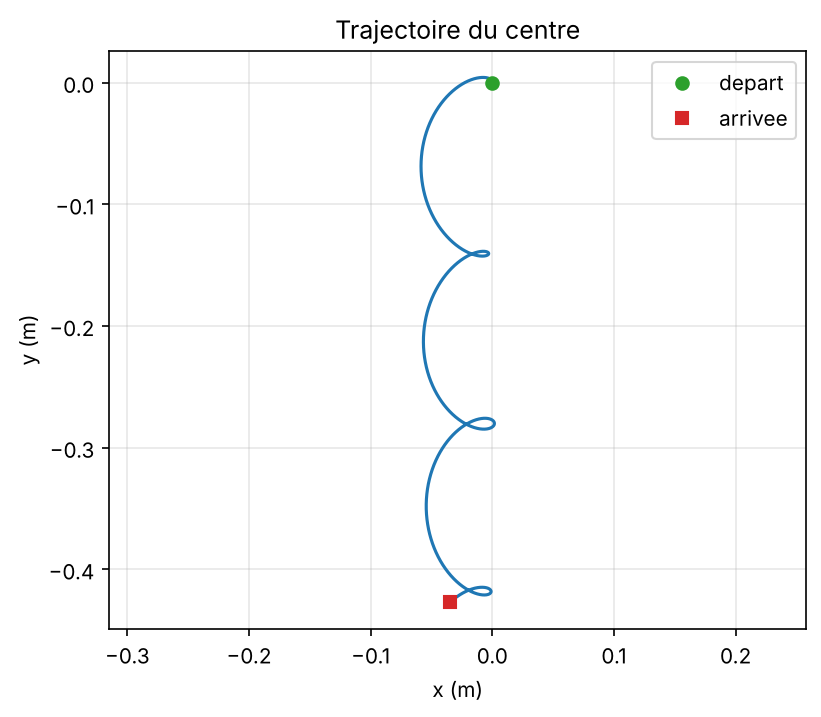
\includegraphics[width=\linewidth]{chapitre4/figures/case_a_trajectory.png}
        \caption{Trajectoire de $G$ dans le plan}
    \end{subfigure}
    \hfill
    \begin{subfigure}{0.52\textwidth}
        \centering
        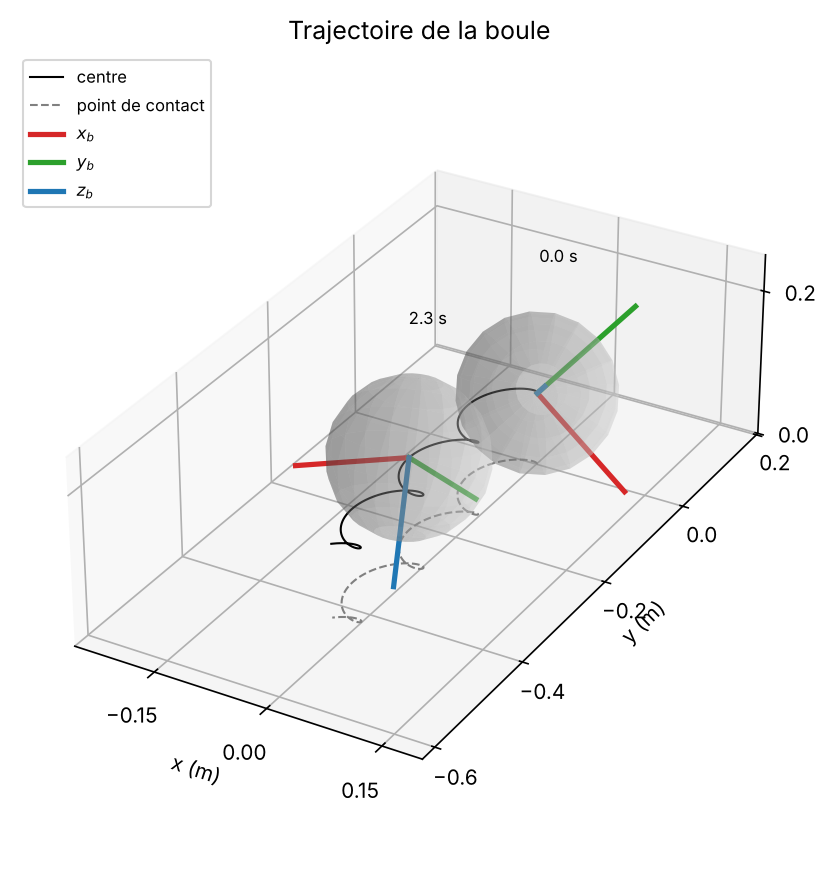
\includegraphics[width=\linewidth]{chapitre4/figures/case_a_trajectory_3d.png}
        \caption{Boule et axes du corps le long de la trajectoire}
    \end{subfigure}
    \caption{Boule anisotrope : trajectoire du centre $G$}
    \label{fig-traj-anisotrope}
\end{figure}

\begin{figure}[H]
    \centering
    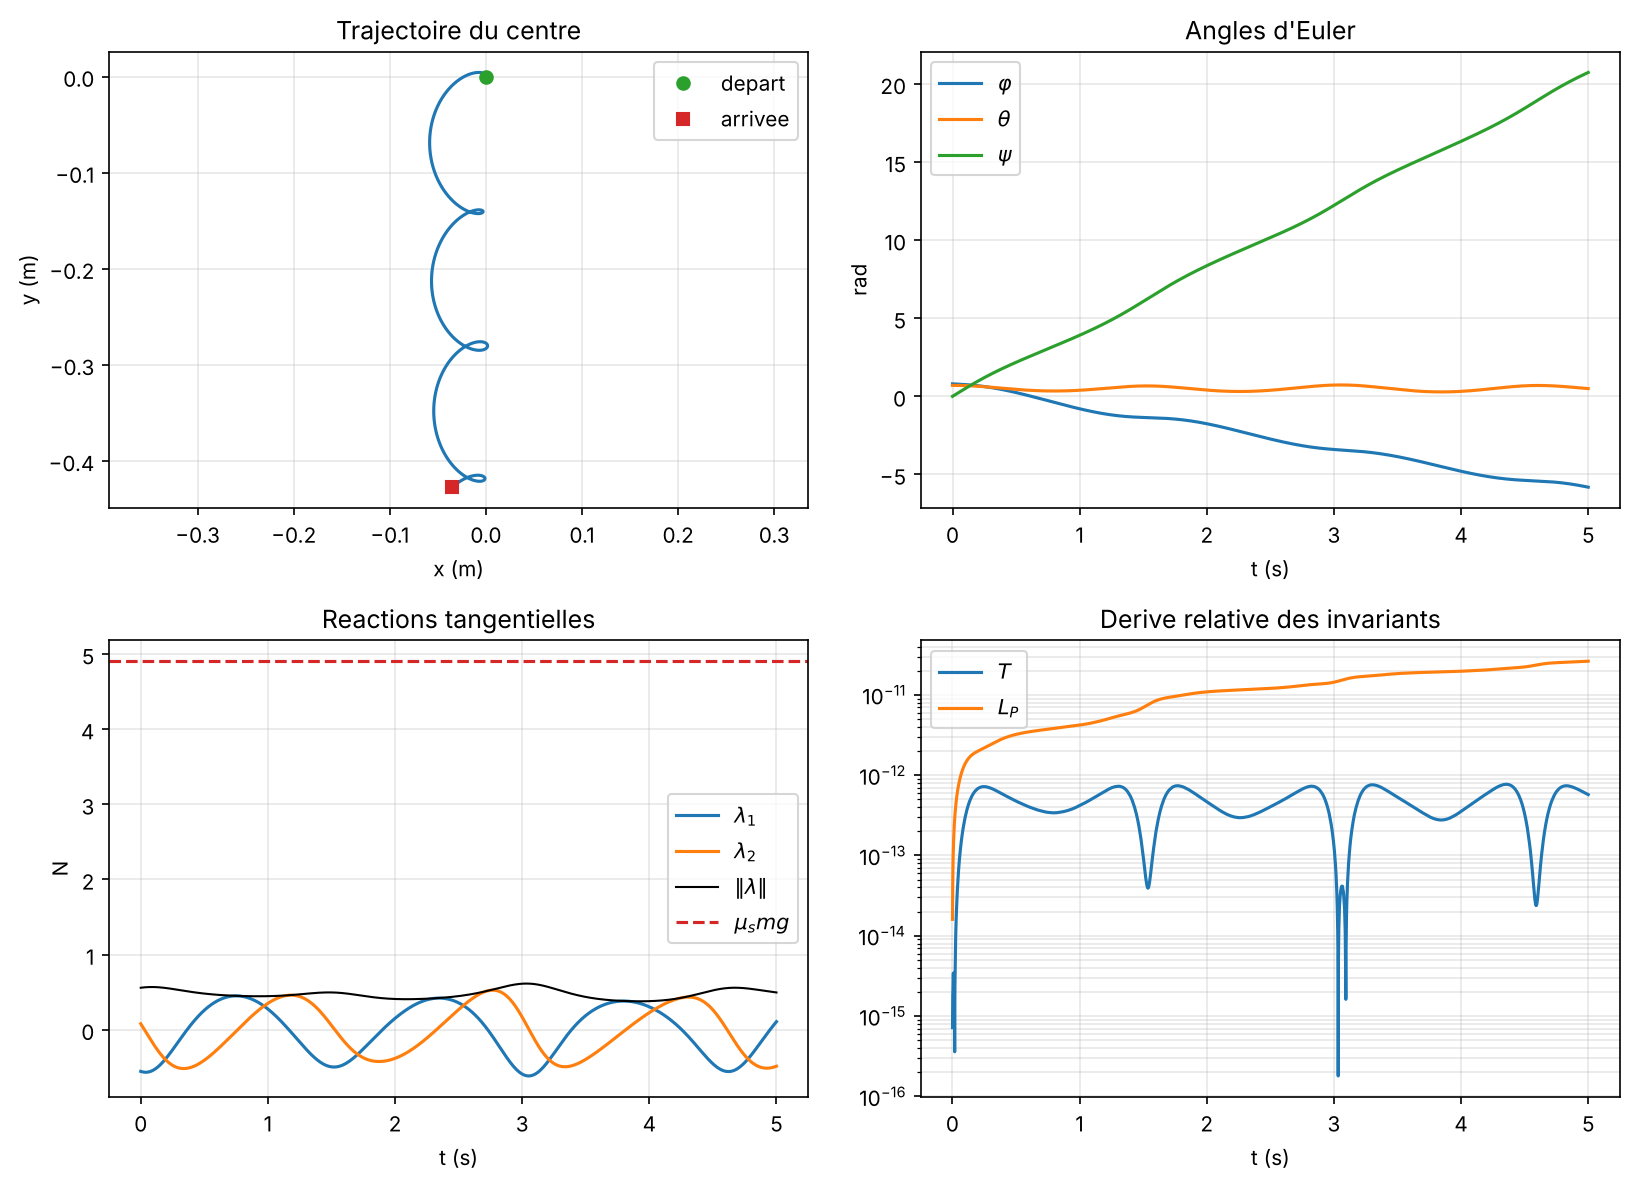
\includegraphics[width=0.9\textwidth]{chapitre4/figures/case_a_summary.png}
    \caption{Boule anisotrope : trajectoire, angles d'Euler, réactions
    tangentielles et dérive des invariants}
    \label{fig-resume-anisotrope}
\end{figure}

\textbf{Contrôles de la simulation :} Les hypothèses de validité sont vérifiées sur
toute la durée :
\begin{itemize}
    \item $|\cos\theta| \geq 0{,}75$ : les angles d'Euler restent loin
    de la singularité.
    \item $\|\vect{\lambda}_k\| \leq 0{,}62$ N $\ll \mu_s\,m\,g$ : pas de
    glissement, et $\mu_s \geq 0{,}07$ suffirait.
    \item Dérives relatives maximales : $8\cdot 10^{-13}$ pour $T$ et
    $3\cdot 10^{-11}$ pour $\vect{L}_P$.
\end{itemize}

% ----------------------------------------------------------------------------
\subsubsection{Boule isotrope}

On prend la boule homogène, $\mat{I}_b = \tfrac25\,m\,a^2\,\Id
= 4\cdot 10^{-3}\,\Id$ kg.m$^2$, avec le même lancer. C'est une sphère dont on connaît a priori la trajectoire, on l'utilise ici juste pour montrer la validité de la simulation.

\begin{proposition}[Boule isotrope]
    Si $\mat{I}_b = I_0\,\Id$, les frottements sont nuls,
    $\vect{\Omega}(t) = \vect{\Omega}_0$, et le centre suit un
    mouvement rectiligne uniforme
    \[
        r(t) = r_0 + a\,t\begin{pmatrix}
            \Omega_{0,y}\\ -\,\Omega_{0,x}
        \end{pmatrix}
    \]
\end{proposition}

\begin{demonstration}
    On note $\vect{F} = N_x\,\vect{e}_x + N_y\,\vect{e}_y$ le
    frottement en $P$. La vitesse du centre de masse s'écrit : 
    \[
        \vect{v}_G = a\,\vect{\Omega}\wedge\vect{e}_z
    \]
    La loi de Newton (ou le théorème de la quantité de mouvement) donne
    \[
        m\,\dot{\vect{v}}_G = \vect{F}
    \]
    Comme $\mat{I}_b = I_0\,\Id$, le moment cinétique en $G$ est
    $\vect{L}_G = I_0\,\vect{\Omega}$. Avec
    $\vect{GP} = -\,a\,\vect{e}_z$, le théorème du moment cinétique
    en $G$ donne
    \[
        I_0\,\dot{\vect{\Omega}}
        = -\,a\,\vect{e}_z\wedge\bigl(\vect{F} + N_z\,\vect{e}_z\bigr)
        = -\,a\,\vect{e}_z\wedge\vect{F}
    \]
    Or, on a : 
    \[
        \dot{\vect{v}}_G = a\,\dot{\vect{\Omega}}\wedge\vect{e}_z
        = -\,\frac{a^2}{I_0}\,(\vect{e}_z\wedge\vect{F})\wedge\vect{e}_z
    \]
    Comme $\vect{F}$ est horizontal,
    $(\vect{e}_z\wedge\vect{F})\wedge\vect{e}_z = \vect{F}$, donc
    \[
        \dot{\vect{v}}_G = -\,\frac{a^2}{I_0}\,\vect{F}
    \]
    En reinjectant dans la loi de Newton, on a :
    \[
        \Bigl(1 + \frac{m\,a^2}{I_0}\Bigr)\vect{F} = \vect{0} \longleftrightarrow \vect{F} = \vect{0}
    \]
    d'où $\vect{F} = \vect{0}$. On en déduit
    $\dot{\vect{\Omega}} = \vect{0}$ et $\dot{\vect{v}}_G = \vect{0}$,
    donc $\vect{v}_G = a\,\vect{\Omega}_0\wedge\vect{e}_z
    = a\,(\Omega_{0,y},\,-\,\Omega_{0,x},\,0)$.
\end{demonstration}

\begin{figure}[H]
    \centering
    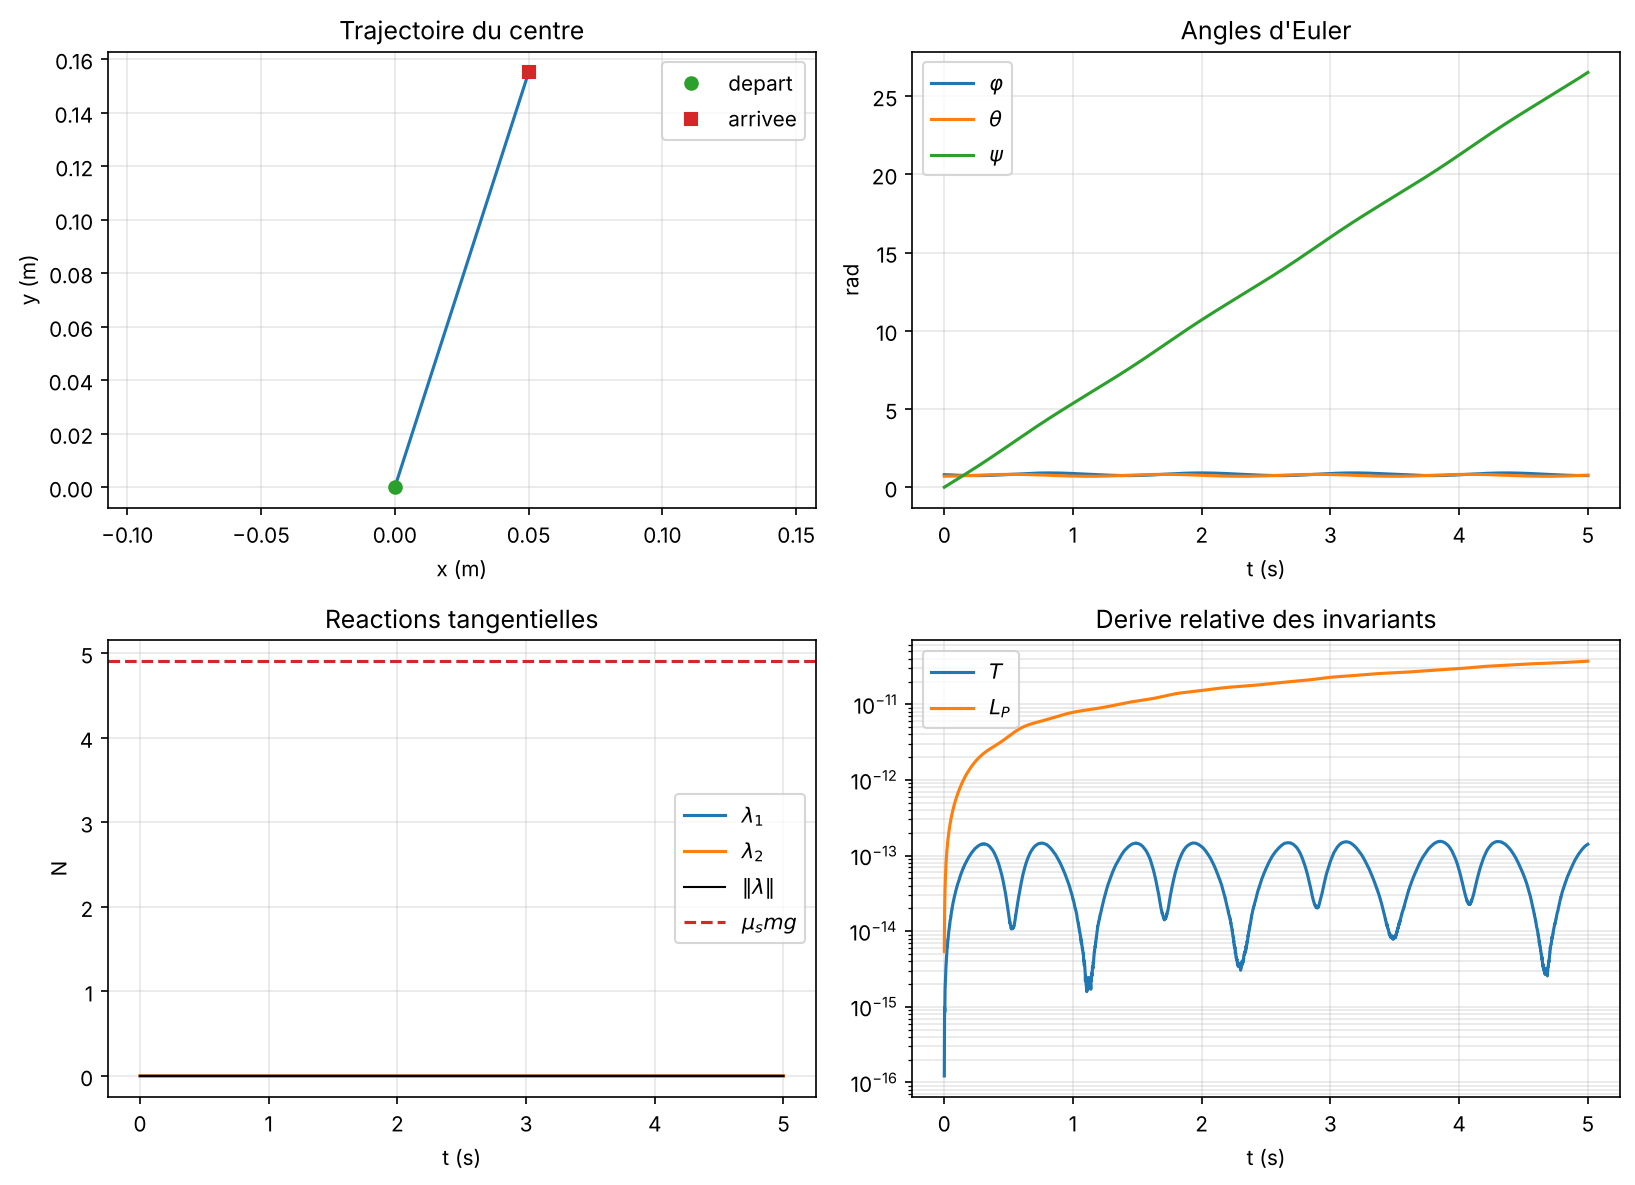
\includegraphics[width=0.9\textwidth]{chapitre4/figures/case_iso_summary.png}
    \caption{Boule isotrope : trajectoire, angles d'Euler, réactions
    tangentielles et dérive des invariants}
    \label{fig-resume-isotrope}
\end{figure}

La simulation retrouve cette solution avec (\cref{fig-resume-isotrope}) :
\[
    \max_k \|\vect{\Omega}_k - \vect{\Omega}_0\| \approx 6\cdot 10^{-11},
    \qquad
    \max_k \|r_k - r(t_k)\| \approx 1{,}5\cdot 10^{-11}\ \text{m},
    \qquad
    \max_k \|\vect{\lambda}_k\| \approx 10^{-16}\ \text{N}
\]
  % II.8. Résultats de la simulation
% ============================================================================
%  Chapitre 4, partie III : Algorithme de simulation en quaternions
% ============================================================================

% ----------------------------------------------------------------------------
\section{Algorithme de simulation - Orientation en quaternions}
% ----------------------------------------------------------------------------

La simulation en angles d'Euler ne tient que tant que
$|\cos\theta| > \varepsilon$. Dans cette partie, on garde la même
dynamique, mais on représente l'orientation par un quaternion unitaire
pour supprimer cette singularité.

% ----------------------------------------------------------------------------
\subsection{Motivation : problème du gimbal lock}

\subsubsection{Perte d'un degré de liberté}

Les colonnes de $\mat{E}$ donnent la vitesse angulaire produite par
chaque angle :
\[
    \pd{\vect{\omega}}{\dot\varphi} = \begin{pmatrix}
        1\\ 0\\ 0
    \end{pmatrix},
    \qquad
    \pd{\vect{\omega}}{\dot\theta} = \begin{pmatrix}
        0\\ c_\varphi\\ -s_\varphi
    \end{pmatrix},
    \qquad
    \pd{\vect{\omega}}{\dot\psi} = \begin{pmatrix}
        -s_\theta\\ s_\varphi c_\theta\\ c_\varphi c_\theta
    \end{pmatrix}
\]
Lorsque $\theta = \pm\pi/2$, la troisième colonne devient
$(\mp 1, 0, 0)$, colinéaire à la première : $\varphi$ et $\psi$
décrivent la même rotation. On perd un degré de liberté, et
$\det\mat{E} = \cos\theta = 0$.

\subsubsection{Conséquence pour la simulation}

La sphère, elle, peut toujours tourner autour de l'axe bloqué. Mais
pour décrire cette rotation en angles d'Euler, il faut
\[
    \dot\alpha = \mat{E}^{-1}\,\vect{\omega}
\]
dont les composantes sont en $1/\cos\theta$. Près de la singularité,
un petit mouvement selon l'axe bloqué donne donc des vitesses
$\dot\varphi$ et $\dot\psi$ très grandes, et des accélérations
$\ddot\alpha$ plus grandes encore. Le système réduit devient mal
conditionné, et le schéma RK4 à pas fixe perd sa précision. Cependant, le mouvement de la sphère n'a rien de particulier. La singularité vient uniquement de la représentation de l'orientation, pas de la physique. Il suffit donc de changer la représentation de l'orientation d'où la solution avec les quaternions.

\subsubsection{Solution par les quaternions}

Un quaternion unitaire $\quat{q}$ décrit l'orientation avec $4$
paramètres liés par $\|\quat{q}\| = 1$. La matrice de rotation
$\mat{R}(\quat{q})$ et la cinématique $\dot{\quat{q}} = \tfrac12\,\quat{q}\quatmul(0,\vect{\omega})$ sont définies pour toute orientation et il n'y a plus de
singularité. Le prix à payer est un paramètre redondant, et une
renormalisation de $\quat{q}$ au cours de la simulation, qui ne sont pas trop chers par rapport à la stabilité que l'on va gagner.

% ----------------------------------------------------------------------------
\subsection{Dynamique du système en représentation quaternionique}

\subsubsection{État}

\textbf{Quaternion des angles d'Euler : } Avec la définition de représentation quaternionique d'une rotation $\theta$ autour d'un axe unitaire $\vect{u}$ du chapitre 2, et avec la convention
$Z$-$Y'$-$X''$, le quaternion est
le produit des trois rotations élémentaires, dans le même ordre que
$\mat{R} = \mat{R}_z(\psi)\,\mat{R}_y(\theta)\,\mat{R}_x(\varphi)$ :
\[
    \quat{q}(\alpha)
    = \Bigl(\cos\tfrac{\psi}{2},\, 0,\, 0,\, \sin\tfrac{\psi}{2}\Bigr)
    \quatmul\Bigl(\cos\tfrac{\theta}{2},\, 0,\, \sin\tfrac{\theta}{2},\, 0\Bigr)
    \quatmul\Bigl(\cos\tfrac{\varphi}{2},\, \sin\tfrac{\varphi}{2},\, 0,\, 0\Bigr)
\]

On décrit l'orientation par $\quat{q}$ et la rotation par la vitesse
angulaire $\vect{\omega}$ exprimée dans le corps. L'état est ainsi 
\[
    Y = (\quat{q},\vect{\omega})\in\R^7, \quad \text{avec} \quad \|\quat{q}\| = 1
\]
soit $7$ nombres pour $6$ degrés de liberté. Comme démontré plus haut avec les angles d'Euler, on peut calculer la position à part. On cherche donc seulement à écrire
\[
    \dot Y = \begin{pmatrix}
        \dot{\quat{q}}\\ \dot{\vect{\omega}}
    \end{pmatrix}
    = \begin{pmatrix}
        \tfrac12\,\quat{q}\quatmul(0,\vect{\omega})\\
        \dot{\vect{\omega}}
    \end{pmatrix}
\]
La première composante est la cinématique quaternionique. Il nous reste à trouver l'équation de $\dot{\vect{\omega}}$.

\subsubsection{Équation de \texorpdfstring{$\dot{\vect{\omega}}$}{omega point}}
Il suffit ici d'utiliser les équations de Gibbs-Appell avec $\vect{\omega}$ comme
pseudo-vitesses.
D'abord, il nous faut retrouver la fonction de Gibbs-Appell en fonction de $\vect{\omega}$.
Soit $\vect{\gamma}$ l'axe vertical vu depuis le corps, $\vect{\gamma}$ s'écrit ainsi dans le repère corps :
\[
    \vect{\gamma} = \mat{R}(\quat{q})^T\vect{e}_z
\]
D'après la fonction de Gibbs-Appell d'un solide, à des termes sans $\dot{\vect{\omega}}$ près, on a :
\[
    \mathcal{G} = \frac{1}{2}\,m\,\|\vect{a}_G\|^2
    + \frac{1}{2}\,\dot{\vect{\omega}}^T\mat{I}_b\,\dot{\vect{\omega}}
    + \dot{\vect{\omega}}\cdot\bigl(\vect{\omega}\wedge
    \mat{I}_b\vect{\omega}\bigr)
\]
On voit que le seul terme qu'il reste à calculer est $\vect{a}_G$.

\textbf{Dérivées de $\mat{R}$ et $\vect{\gamma}$ : } Comme
$\vect{\Omega} = \mat{R}\,\vect{\omega}$,
\[
    \dot{\mat{R}} = \hatx{\vect{\Omega}}\,\mat{R}
    = \mat{R}\,\hatx{\vect{\omega}}
\]
et comme $\vect{e}_z$ est fixe,
\[
    \dot{\vect{\gamma}} = \dot{\mat{R}}^T\vect{e}_z
    = -\,\hatx{\vect{\omega}}\,\mat{R}^T\vect{e}_z
    = -\,\vect{\omega}\wedge\vect{\gamma}
    = \vect{\gamma}\wedge\vect{\omega}
\]

\textbf{Accélération du centre : } D'après le roulement, avec
$\vect{\Omega} = \mat{R}\,\vect{\omega}$ et
$\vect{e}_z = \mat{R}\,\vect{\gamma}$, on a :
\[
    \vect{v}_G = a\,\vect{\Omega}\wedge\vect{e}_z
    = a\,\mat{R}\vect{\omega}\wedge\mat{R}\vect{\gamma}
\]
puis, comme une rotation conserve le produit vectoriel,
\[
    \vect{v}_G = a\,\mat{R}\,(\vect{\omega}\wedge\vect{\gamma})
\]
En dérivant ce terme, on a l'accélération :
\[
    \vect{a}_G = a\,\mat{R}\Bigl(
    \vect{\omega}\wedge(\vect{\omega}\wedge\vect{\gamma})
    + \dot{\vect{\omega}}\wedge\vect{\gamma}
    + \vect{\omega}\wedge(\vect{\gamma}\wedge\vect{\omega})\Bigr)
\]
Le premier et le dernier terme s'annulent, car
$\vect{\omega}\wedge\vect{\gamma} + \vect{\gamma}\wedge\vect{\omega}
= \vect{0}$, d'où
\[
    \vect{a}_G = a\,\mat{R}\,(\dot{\vect{\omega}}\wedge\vect{\gamma})
\]
Comme $\mat{R}$ conserve la norme,
$\|\vect{a}_G\| = a\,\|\dot{\vect{\omega}}\wedge\vect{\gamma}\|$.

\begin{proposition}[Fonction de Gibbs-Appell de la sphère avec $\vect{\omega}$ comme pseudo-vitesse]
    Avec $\vect{\omega}$ comme pseudo-vitesse, la fonction de
    Gibbs-Appell de la sphère s'écrit :
    \[
        \mathcal{G} = \tfrac12\,m\,a^2\,
        \|\dot{\vect{\omega}}\wedge\vect{\gamma}\|^2
        + \tfrac12\,\dot{\vect{\omega}}^T\mat{I}_b\,\dot{\vect{\omega}}
        + \dot{\vect{\omega}}\cdot(\vect{\omega}\wedge\mat{I}_b\,
        \vect{\omega})
    \]
\end{proposition}
Ensuite, on développe le premier terme en utilisant la formule de la
norme d'un produit vectoriel
$\|\vect{u}\wedge\vect{v}\|^2 = \|\vect{u}\|^2\,\|\vect{v}\|^2
- (\vect{u}\cdot\vect{v})^2$ avec $\|\vect{\gamma}\| = 1$ :
\[
    \|\dot{\vect{\omega}}\wedge\vect{\gamma}\|^2
    = \|\dot{\vect{\omega}}\|^2
    - (\dot{\vect{\omega}}\cdot\vect{\gamma})^2
    = \dot{\vect{\omega}}^T\bigl(\Id - \vect{\gamma}\vect{\gamma}^T
    \bigr)\dot{\vect{\omega}}
\]
On réécrit la fonction de Gibbs-Appell sous la forme :
\[
    \mathcal{G} = \tfrac12\,\dot{\vect{\omega}}^T\mat{K}(\vect{\gamma})
    \,\dot{\vect{\omega}}
    + \dot{\vect{\omega}}\cdot(\vect{\omega}\wedge\mat{I}_b\,
    \vect{\omega}) \quad \text{avec} \quad
    \mat{K}(\vect{\gamma}) = \mat{I}_b
    + m\,a^2\,\bigl(\Id - \vect{\gamma}\vect{\gamma}^T\bigr)
\]
Le potentiel $V = m g a$ est constant et aucune force non
conservative n'est appliquée, donc $\mathcal{Q} = 0$. On en déduit
l'équation de Gibbs-Appell :
\[
    \pd{\mathcal{G}}{\dot{\vect{\omega}}}
    = \mat{K}(\vect{\gamma})\,\dot{\vect{\omega}}
    + \vect{\omega}\wedge\mat{I}_b\,\vect{\omega} = \vect{0}
\]
\begin{proposition}[Inversibilité de $\mat{K}(\vect{\gamma})$]
    La matrice $\mat{K}(\vect{\gamma})$ est symétrique, définie positive donc inversible.
\end{proposition}
\begin{demonstration}
    On voit bien que $\mat{K}(\vect{\gamma})$ est symétrique,
    et pour tout $\vect{v}\neq\vect{0}$,
    \[
        \vect{v}^T\mat{K}(\vect{\gamma})\,\vect{v}
        = \vect{v}^T\mat{I}_b\,\vect{v}
        + m\,a^2\,\|\vect{v}\wedge\vect{\gamma}\|^2
        \geq \vect{v}^T\mat{I}_b\,\vect{v} > 0
    \]
    car $\mat{I}_b$ est définie positive. $\mat{K}$ est donc inversible.
\end{demonstration}

\begin{proposition}[Dynamique en quaternions]
    Avec
    \[
        \mat{K}(\vect{\gamma}) = \mat{I}_b
        + m\,a^2\,\bigl(\Id - \vect{\gamma}\vect{\gamma}^T\bigr)
    \]
    on a
    \[
        \mat{K}(\vect{\gamma})\,\dot{\vect{\omega}}
        = -\,\vect{\omega}\wedge\mat{I}_b\,\vect{\omega}
    \]
\end{proposition}

On a donc la dynamique
\[
    \dot Y = f(Y)= \begin{pmatrix}
        \tfrac12\,\quat{q}\quatmul(0,\vect{\omega})\\
        -\,\mat{K}(\vect{\gamma})^{-1}
        \bigl(\vect{\omega}\wedge\mat{I}_b\,\vect{\omega}\bigr)
    \end{pmatrix}
\]
définie pour toute orientation, sans condition sur $\cos\theta$.

\subsubsection{Position et frottements}

Une fois $Y$ connu, la position et les frottements s'en déduisent sans
nouvelle équation. On repasse dans le repère du sol avec
$\vect{\Omega} = \mat{R}\,\vect{\omega}$. On a, avec
$\dot{\mat{R}} = \mat{R}\,\hatx{\vect{\omega}}$,
\[
    \dot{\vect{\Omega}} = \mat{R}\,(\vect{\omega}\wedge\vect{\omega})
    + \mat{R}\,\dot{\vect{\omega}}
    = \mat{R}\,\dot{\vect{\omega}}
\]

\textbf{Position : }
\[
    \dot{\vect{r}} = \vect{v}_G = \begin{pmatrix}
        \dot x\\ \dot y\\ 0
    \end{pmatrix}
    = a\,\vect{\Omega}\wedge\vect{e}_z
    = a\begin{pmatrix}
        \Omega_y\\ -\,\Omega_x\\ 0
    \end{pmatrix}
\]
On peut simplement calculer $\vect{r}$ avec une quadrature. 

\textbf{Frottements : } D'après la loi de Newton en $x$ et $y$,
$(N_x, N_y, 0) = m\,\vect{a}_G$. Avec
$\vect{a}_G = a\,\mat{R}\,(\dot{\vect{\omega}}\wedge\vect{\gamma})$ et
$\mat{R}\,\vect{\gamma} = \vect{e}_z$ : 
\[
    \vect{a}_G = a\,\dot{\vect{\Omega}}\wedge\vect{e}_z
    = a\begin{pmatrix}
        \dot\Omega_y\\ -\,\dot\Omega_x\\ 0
    \end{pmatrix}
\]

\begin{proposition}[Position et frottements]
    Avec $\vect{\Omega} = \mat{R}(\quat{q})\,\vect{\omega}$ et
    $\dot{\vect{\Omega}} = \mat{R}(\quat{q})\,\dot{\vect{\omega}}$,
    \[
        \dot x = a\,\Omega_y,
        \qquad
        \dot y = -\,a\,\Omega_x,
        \qquad
        N_x = m\,a\,\dot\Omega_y,
        \qquad
        N_y = -\,m\,a\,\dot\Omega_x
    \]
    et $N_z = m g$. Le non-glissement se vérifie a posteriori par
    \[
        \sqrt{N_x^2 + N_y^2} \leq \mu_s\,m\,g
    \]
\end{proposition}

% ----------------------------------------------------------------------------
\subsection{Schéma numérique}

On reprend le schéma RK4 de la partie II pour $\dot Y = f(Y)$, mais
cette fois-ci $Y = (\quat{q},\vect{\omega})$. La seule nouveauté est la
renormalisation de $\quat{q}$ à chaque pas.

\subsubsection{Conditions initiales}

\begin{proposition}[Conditions initiales]
    Les conditions initiales de cette dynamique sont
    $(r_0, \quat{q}(0), \vect{\omega}_0)$.
\end{proposition}

Comme en partie II, on se donne la position $r_0$, l'orientation
$\alpha_0$ et la vitesse angulaire $\vect{\Omega}_0$ dans $\rep{s}$.
On en déduit
\[
    \quat{q}(0) = \quat{q}(\alpha_0),
    \qquad
    \vect{\omega}_0 = \mat{R}\bigl(\quat{q}(0)\bigr)^T\vect{\Omega}_0
\]
Contrairement aux angles d'Euler, il n'y a aucune condition sur
$\cos\theta_0$ : on n'inverse plus $\mat{E}_s$. Enfin,
$\dot{\vect{\omega}}_0$ et les frottements initiaux s'obtiennent en
faisant les mêmes calculs que les étapes 3 et 4.

\subsubsection{Choix du pas}

\subsubsection{Schéma RK4 pour simuler le système}

\paragraph{Étape 1 : Orientation} Avec
$Y_k = (\quat{q}_k,\vect{\omega}_k)$, on évalue $f$ en quatre états
intermédiaires du pas,
\[
    Y^{(1)} = Y_k,
    \qquad
    Y^{(2)} = Y_k + \tfrac{h}{2}\,\vect{p}_1,
    \qquad
    Y^{(3)} = Y_k + \tfrac{h}{2}\,\vect{p}_2,
    \qquad
    Y^{(4)} = Y_k + h\,\vect{p}_3
\]
où $Y^{(i)} = (\quat{q}^{(i)},\vect{\omega}^{(i)})$ et
\[
    \vect{p}_i = f\bigl(Y^{(i)}\bigr)
    = \begin{pmatrix}
        \dot{\quat{q}}^{(i)}\\ \dot{\vect{\omega}}^{(i)}
    \end{pmatrix},
    \qquad
    \dot{\quat{q}}^{(i)} = \tfrac12\,\quat{q}^{(i)}\quatmul
    (0,\vect{\omega}^{(i)})
\]
avec
\[
    \mat{K}\bigl(\vect{\gamma}^{(i)}\bigr)\,\dot{\vect{\omega}}^{(i)}
    = -\,\vect{\omega}^{(i)}\wedge\mat{I}_b\,\vect{\omega}^{(i)},
    \qquad
    \vect{\gamma}^{(i)} = \mat{R}\bigl(\quat{q}^{(i)}\bigr)^T\vect{e}_z
\]
On obtient alors le nouvel état :
\[
    \quat{q}_{k+1} = \quat{q}_k + \tfrac{h}{6}\,\bigl(\dot{\quat{q}}^{(1)}
    + 2\,\dot{\quat{q}}^{(2)} + 2\,\dot{\quat{q}}^{(3)}
    + \dot{\quat{q}}^{(4)}\bigr),
    \qquad
    \vect{\omega}_{k+1} = \vect{\omega}_k + \tfrac{h}{6}\,\bigl(
    \dot{\vect{\omega}}^{(1)} + 2\,\dot{\vect{\omega}}^{(2)}
    + 2\,\dot{\vect{\omega}}^{(3)} + \dot{\vect{\omega}}^{(4)}\bigr)
\]

\paragraph{Étape 2 : Renormalisation} La dynamique conserve
$\|\quat{q}\| = 1$, mais pas le schéma : l'erreur est en
$O(h^5)$ sur un pas et s'accumule au cours de la simulation. Il nous faut alors 
renormaliser à chaque pas : 
\[
    \quat{q}_{k+1} \longleftarrow
    \frac{\quat{q}_{k+1}}{\|\quat{q}_{k+1}\|}
\]
L'écart $\bigl|\,\|\quat{q}_{k+1}\| - 1\,\bigr|$ avant renormalisation
reste de l'ordre de l'erreur du schéma.

\paragraph{Étape 3 : Accélération} On résout l'équation de
$\dot{\vect{\omega}}$ au nouvel état :
\[
    \mat{K}(\vect{\gamma}_{k+1})\,\dot{\vect{\omega}}_{k+1}
    = -\,\vect{\omega}_{k+1}\wedge\mat{I}_b\,\vect{\omega}_{k+1},
    \qquad
    \vect{\gamma}_{k+1} = \mat{R}(\quat{q}_{k+1})^T\vect{e}_z
\]
C'est la seconde moitié de $f(Y_{k+1})$, réutilisée comme
$\vect{p}_1$ au pas suivant.

\paragraph{Étape 4 : Position et frottements} En parallèle avec
l'étape 1, on calcule des poids RK4 pour $r$ avec
$\vect{g}_i = a\,\bigl(\Omega_y^{(i)}, -\,\Omega_x^{(i)}\bigr)$ et
$\vect{\Omega}^{(i)} = \mat{R}\bigl(\quat{q}^{(i)}\bigr)\,
\vect{\omega}^{(i)}$, tels que :
\[
    r_{k+1} = r_k + \tfrac{h}{6}\,\bigl(\vect{g}_1 + 2\,\vect{g}_2
    + 2\,\vect{g}_3 + \vect{g}_4\bigr)
\]
puis, avec $\dot{\vect{\Omega}}_{k+1} = \mat{R}(\quat{q}_{k+1})\,
\dot{\vect{\omega}}_{k+1}$,
\[
    N_{x,k+1} = m\,a\,\dot\Omega_{y,k+1},
    \qquad
    N_{y,k+1} = -\,m\,a\,\dot\Omega_{x,k+1}
\]

% ----------------------------------------------------------------------------
\subsection{Architecture de la simulation}

Voici l'architecture de la simulation prête à implémenter avec
l'orientation représentée par un quaternion unitaire.

\begin{figure}[H]
    \centering
    \begin{tikzpicture}[>=Stealth,
        bloc/.style={draw, thick, rounded corners=2pt, align=center,
            fill=coulprop!6, draw=coulprop, inner sep=4pt,
            font=\small},
        ctrl/.style={bloc, fill=couldef!8, draw=couldef},
        stop/.style={bloc, fill=coulthm!8, draw=coulthm},
        es/.style={bloc, fill=gray!8, draw=gray},
        fl/.style={->, thick},
        lab/.style={font=\footnotesize, fill=white, inner sep=1pt}]

        \node[es] (in) at (0,0) {Entrées : $m$, $a$, $\mat{I}_b$,
            $\mu_s$ ; $r_0$, $\alpha_0$, $\vect{\Omega}_0$ ; $h$, $N$};
        \node[bloc] (init) at (0,-1.3)
            {Initialisation : $\quat{q}(0) = \quat{q}(\alpha_0)$,
            \quad $\vect{\omega}_0 = \mat{R}\bigl(\quat{q}(0)\bigr)^T
            \vect{\Omega}_0$, \quad
            $Y_0 = \bigl(\quat{q}(0),\vect{\omega}_0\bigr)$};
        \node[bloc] (f) at (0,-3.3)
            {Évaluation de $f$ en $Y^{(i)}$, $i = 1,\dots,4$ :\\[2pt]
            $\dot{\quat{q}}^{(i)} = \tfrac12\,\quat{q}^{(i)}\quatmul
            (0,\vect{\omega}^{(i)})$\\[2pt]
            $\mat{R}\bigl(\quat{q}^{(i)}\bigr)$
            $\;\to\;$ $\vect{\gamma}^{(i)}$
            $\;\to\;$ $\mat{K}\bigl(\vect{\gamma}^{(i)}\bigr)\,
            \dot{\vect{\omega}}^{(i)}
            = -\,\vect{\omega}^{(i)}\wedge\mat{I}_b\,\vect{\omega}^{(i)}$};
        \node[bloc] (rk) at (-2.9,-5.5)
            {Étape 1 : $Y_{k+1}$ par RK4\\[2pt]
            Étape 2 : $\quat{q}_{k+1} \leftarrow
            \quat{q}_{k+1}/\|\quat{q}_{k+1}\|$\\[2pt]
            Étape 3 : $\dot{\vect{\omega}}_{k+1}$};
        \node[bloc] (rl) at (2.9,-5.5)
            {Étape 4 : $r_{k+1}$ avec les $\vect{g}_i$,\\[2pt]
            $N_{x,k+1}$, $N_{y,k+1}$};
        \node[ctrl] (c) at (0,-7.4)
            {Contrôles : $T$, $\vect{L}_P$ conservés ;
            $\sqrt{N_{x,k+1}^2 + N_{y,k+1}^2} \leq \mu_s\,m\,g$};
        \node[stop] (arret) at (-3.6,-9.3)
            {Arrêt : simulation\\non valide};
        \node[es] (out) at (3.6,-9.3)
            {Sorties : $r_k$, $\quat{q}_k$, $\vect{\omega}_k$,
            $(N_x, N_y)_k$,\\
            $k = 0,\dots,N$};

        \draw[fl] (in) -- (init);
        \draw[fl] (init) -- (f);
        \draw[fl] (f) -- (rk);
        \draw[fl] (f) -- (rl);
        \draw[fl] (rk) -- (c);
        \draw[fl] (rl) -- (c);
        \draw[fl, coulthm] (c) -- node[lab, pos=0.45, left=2pt]
            {non} (arret);
        \draw[fl] (c) -- node[lab, pos=0.45, right=2pt]
            {oui, $k = N$} (out);
        \coordinate (droite) at (6.4,0);
        \draw[fl] (c.east) -- (c.east -| droite) -- (f.east -| droite)
            node[lab, pos=0.5, left=2pt, align=right]
            {oui,\\$k \leftarrow k+1$} -- (f.east);

        \begin{scope}[on background layer]
            \node[draw=gray, dashed, rounded corners, inner sep=7pt,
                fit=(f) (rk) (rl) (c) (c.east -| droite)] (boucle) {};
        \end{scope}
        \node[font=\footnotesize, gray, anchor=south west]
            at (boucle.north west) {boucle sur $k$};
    \end{tikzpicture}
    \caption{Architecture de la simulation de la sphère de Chaplygin
    en quaternions}
\end{figure}

Par rapport aux angles d'Euler, le contrôle $|\cos\theta| > \varepsilon$
disparaît, et l'étape de renormalisation s'ajoute.

\subsection{Validation de la simulation}
\subsubsection{Écart avec le modèle en angles d'Euler}

On relance la boule anisotrope de la partie précédente
(figure~\ref{fig-traj-anisotrope}), avec les mêmes paramètres et le même
pas $h$, une fois avec le modèle en angles d'Euler et une fois avec le
modèle en quaternions. Sur ce lancer, $|\cos\theta| \geq 0{,}74$ et les deux modèles décrivent la même
dynamique. Les deux simulations doivent donc donner le même résultat, à l'erreur du schéma près.
\paragraph{Écarts mesurés : } on note avec un indice $E$ (resp. $Q$) les
grandeurs calculées en angles d'Euler (resp. en quaternions), et on
mesure à chaque pas
\[
    \|r_k^E - r_k^Q\|,
    \qquad
    \|\mat{R}_k^E - \mat{R}_k^Q\|_F,
    \qquad
    \|(N_x, N_y)_k^E - (N_x, N_y)_k^Q\|
\]
où $\|\cdot\|_F$ est la norme de Frobenius. Sur les $5$ s de simulation,
ces écarts restent inférieurs à $1{,}1\cdot 10^{-11}$ m,
$2{,}2\cdot 10^{-11}$ et $6{,}7\cdot 10^{-12}$ N respectivement
(figure~\ref{fig-ecart-euler-quat}). La dérive relative de l'énergie
reste de l'ordre de $10^{-12}$ pour les deux modèles.

\begin{figure}[H]
    \centering
    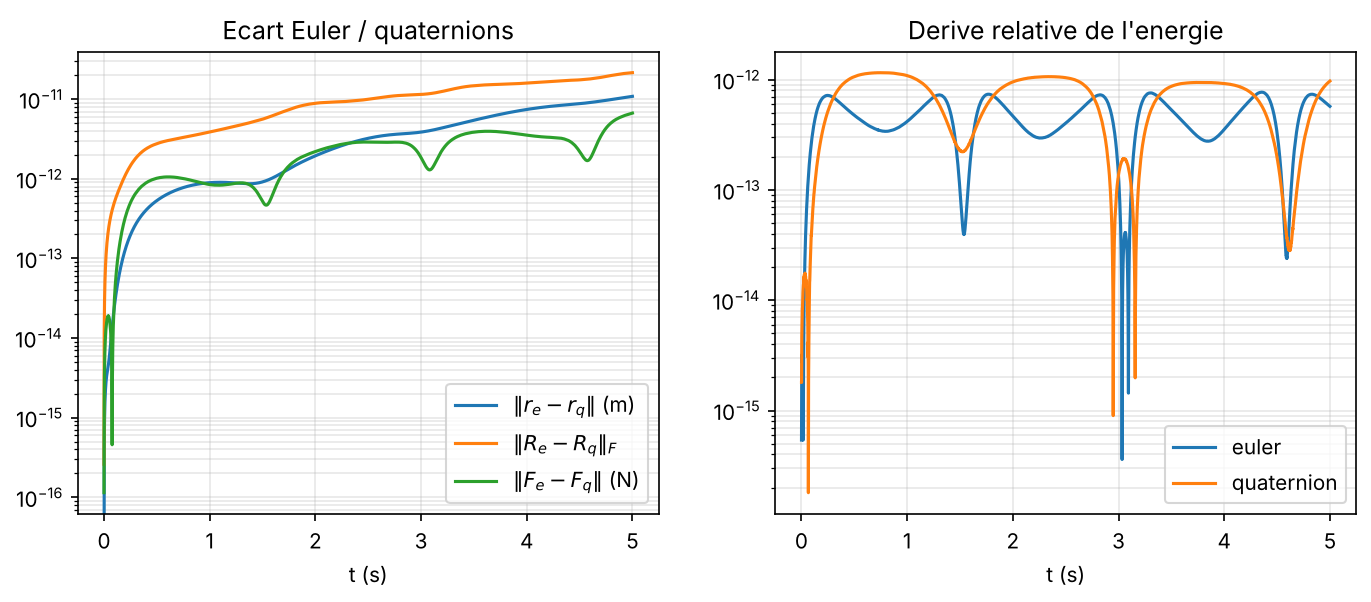
\includegraphics[width=0.95\textwidth]{chapitre4/figures/validation_case_a_errors.png}
    \caption{Boule anisotrope : écart entre les simulations en angles
    d'Euler et en quaternions, et dérive relative de l'énergie}
    \label{fig-ecart-euler-quat}
\end{figure}

Loin de la singularité, la simulation en quaternions redonne donc les
résultats de la simulation en angles d'Euler.

\paragraph{Près du gimbal lock}

On lance maintenant la même boule avec un tangage proche de $90^\circ$ :
\[
    \alpha_0 = (0;\ 90^\circ - 0{,}4^\circ;\ 0),
    \qquad
    \vect{\Omega}_0 = (5;\ 1;\ 2) \text{ rad.s}^{-1}
\]
avec le même pas $h$ et la même durée. On peut par partir de gimbal lock car la simulation en angles d'Euler ne pourrait pas se lancer, mais on peut partir de son voisinage et lui donne de la vitesse pour atteindre gimbal lock.

\textbf{Trajectoire et angles : } les deux simulations coïncident jusqu'à
$t \approx 1{,}84$ s (figure~\ref{fig-gimbal-traj}). Les angles calculés en angles d'Euler s'écartent alors de ceux calculés en quaternions, et la trajectoire de $G$ avec eux :
l'écart atteint $50$ cm à $t = 5$ s.

\begin{figure}[H]
    \centering
    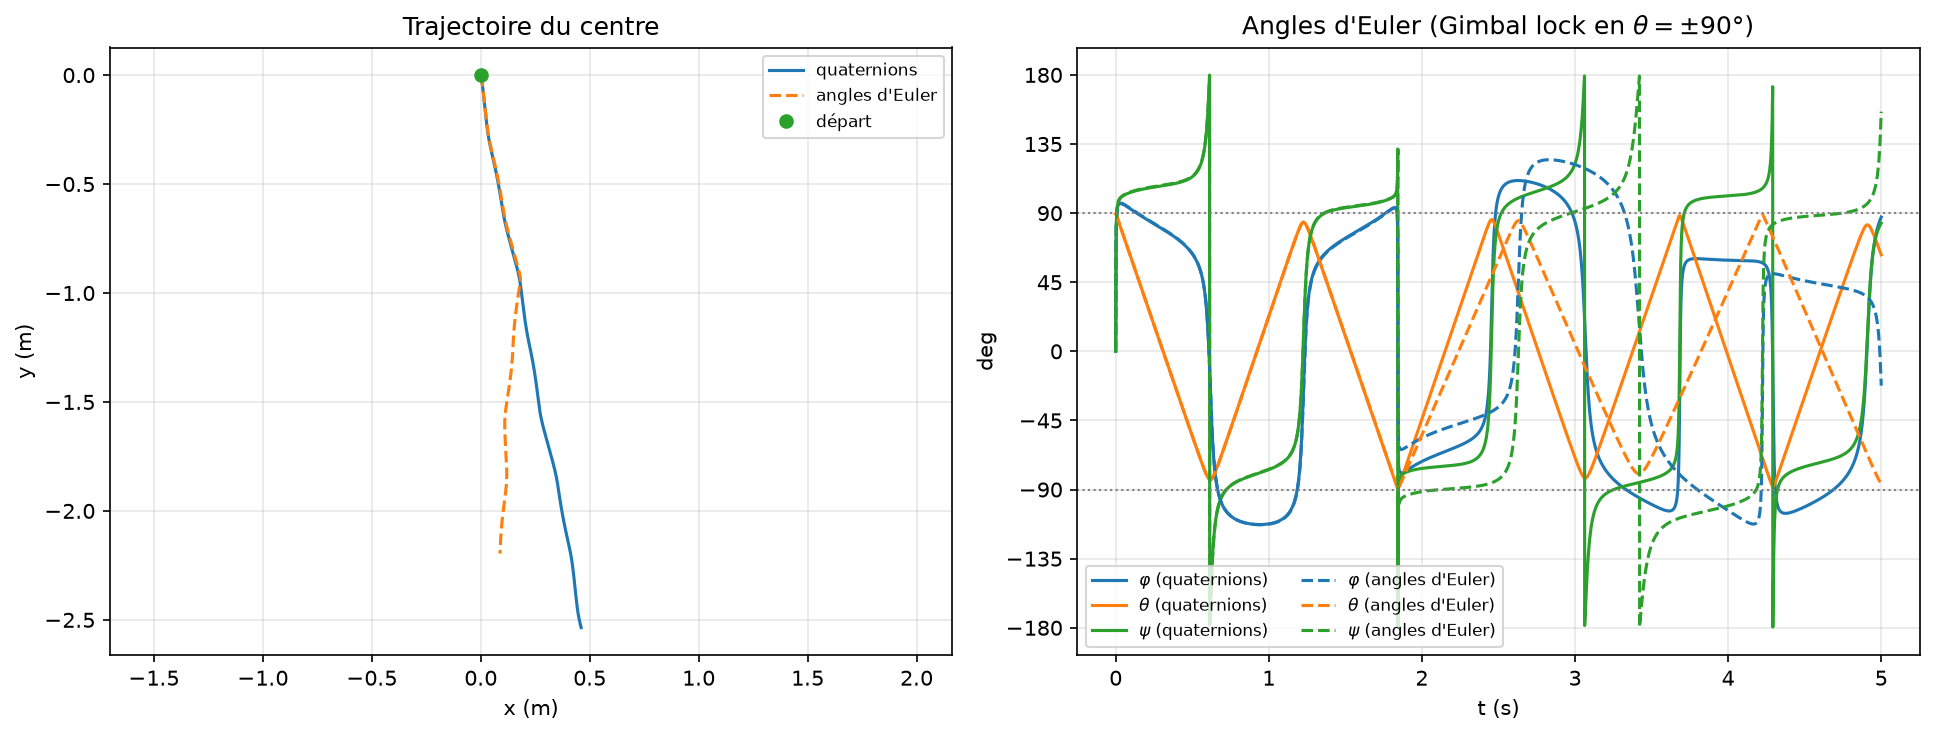
\includegraphics[width=\textwidth]{chapitre4/figures/case_b_euler_vs_quat.png}
    \caption{Près du gimbal lock : trajectoire de $G$ et angles d'Euler,
    calculés en quaternions (trait plein) et en angles d'Euler (tirets)}
    \label{fig-gimbal-traj}
\end{figure}

\textbf{Contrôles : } en quaternions, les dérives relatives de $T$ et de
$\vect{L}_P$ restent de l'ordre de $10^{-12}$
(figure~\ref{fig-gimbal-controles}). En angles d'Euler, les dérives de
$T$ et de $\vect{L}_P$ valent déjà quelques $10^{-3}$ dès le premier pas,
puisqu'on part près de la singularité, puis sautent à $43\ \%$ et
$33\ \%$ au passage de $t \approx 1{,}84$ s. L'erreur du schéma utilisant les angles d'Euler s'accumule dès les premiers pas près de la singularité, donc, pour la trajectoire, ce n'est pas forcément fiable pour la simulation en angles d'Euler.

En revanche, les deux autres contrôles passent : on a toujours
$|\cos\theta| > \varepsilon = 10^{-3}$, et
$\|(N_x, N_y)\| \leq 0{,}47$ N reste loin de $\mu_s\,m\,g \approx 4{,}9$ N.
La simulation en angles d'Euler est donc déclarée valide alors qu'elle
est fausse, on ne peut voir les erreurs qu'à travers les conservations.

\begin{figure}[H]
    \centering
    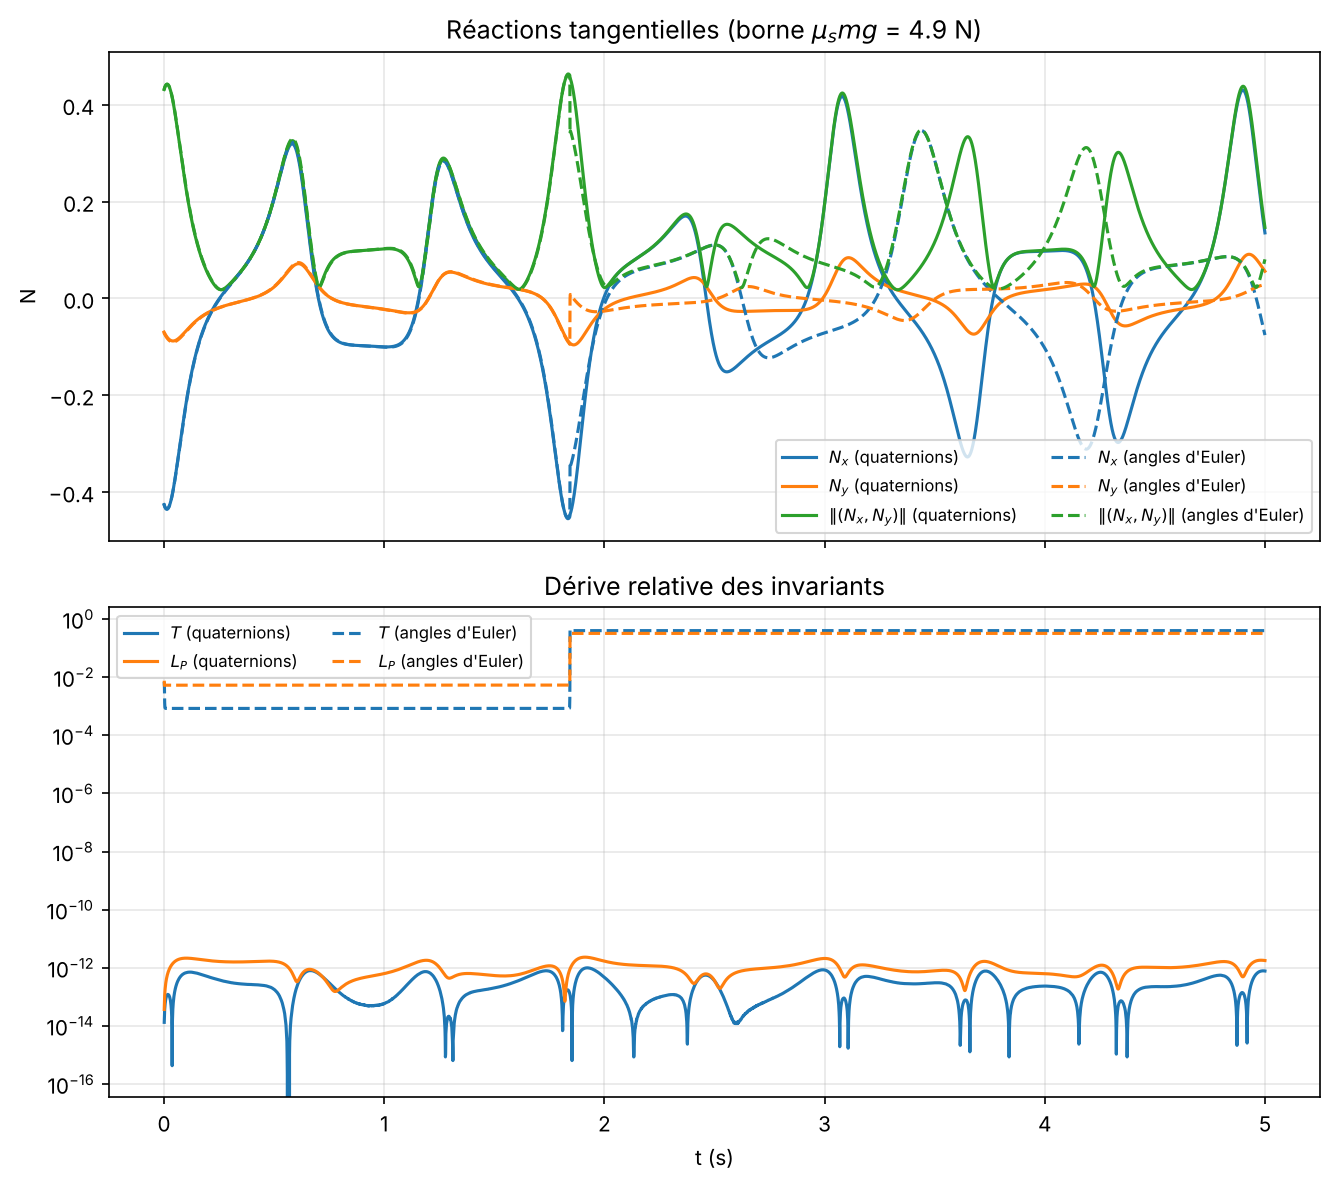
\includegraphics[width=0.8\textwidth]{chapitre4/figures/case_b_controls.png}
    \caption{Près du gimbal lock : réactions tangentielles et dérive
    relative des invariants, en quaternions (trait plein) et en angles
    d'Euler (tirets)}
    \label{fig-gimbal-controles}
\end{figure}

Près de la singularité, seule la simulation en quaternions reste fiable.
 % III. Algorithme de simulation en quaternions

% Parties suivantes, à discuter :
% \input{chapitre4/derive}      % III. Dérive de la contrainte
% \input{chapitre4/validation}  % IV.  Validation et résultats


\end{document}
